\chapter{Empirical Analysis - Machine Learning Implementation}
\label{chap:four}
This chapter focuses on the main part of this thesis, particularly on the practical example of machine learning implementation. The machine learning framework deployed in this thesis is shown in \autoref{fig:mlframe}.
\begin{itemize}\setlength\itemsep{0em}
\item \textbf{Data Exploration} - this part of the framework is focused on the exploration of the data in order to infer some insights about the data quality, distribution of the variables, statistical testing or association analysis.
\item \textbf{Data Split} - this part of the framework is focused on the splitting of the data which are used separaterly in diferrent tasks such as model training, model selection and model evaluation.
\item \textbf{Optimal Binning and WoE Encoding} - this part of the framework is focused on the optimal binning and the WoE encoding of the features as the main part of the feature preprocessing.
\item \textbf{Feature Selection} - this part of the framework is focused on the feature selection in order to reduce the dimensionality of the data and to improve the performance of the machine learning models - each input model estimator is tuned with Bayesian Optimization.
\item \textbf{Model Selection} - this part of the framework is focused on the model selection in order to find the best model based on the ranking - each input model is tuned with Bayesian Optimization on the subsets of selected features.
\item \textbf{Model Building (Evaluation)} - this part of the framework is focused on the recalibration of the final model by re-training it on the joined training and validation sets, which will be further evaluated.
\item \textbf{Model Evaluation} - this part of the framework is focused on the evaluation of the final model on the unseen data from test set.
\item \textbf{Model Building (Deployment)} - this part of the framework is focused on the final recalibration of the final model by re-training it on the joined training, validation and test sets, which will be further deployed into a production.
\item \textbf{Model Deployment} - this part of the framework is focused on the deployment of the final model into a production as a web application.
\end{itemize}

\begin{figure}[H]
\centering
\caption{Machine Learning Framework}\vspace{0.5em}
\label{fig:mlframe}
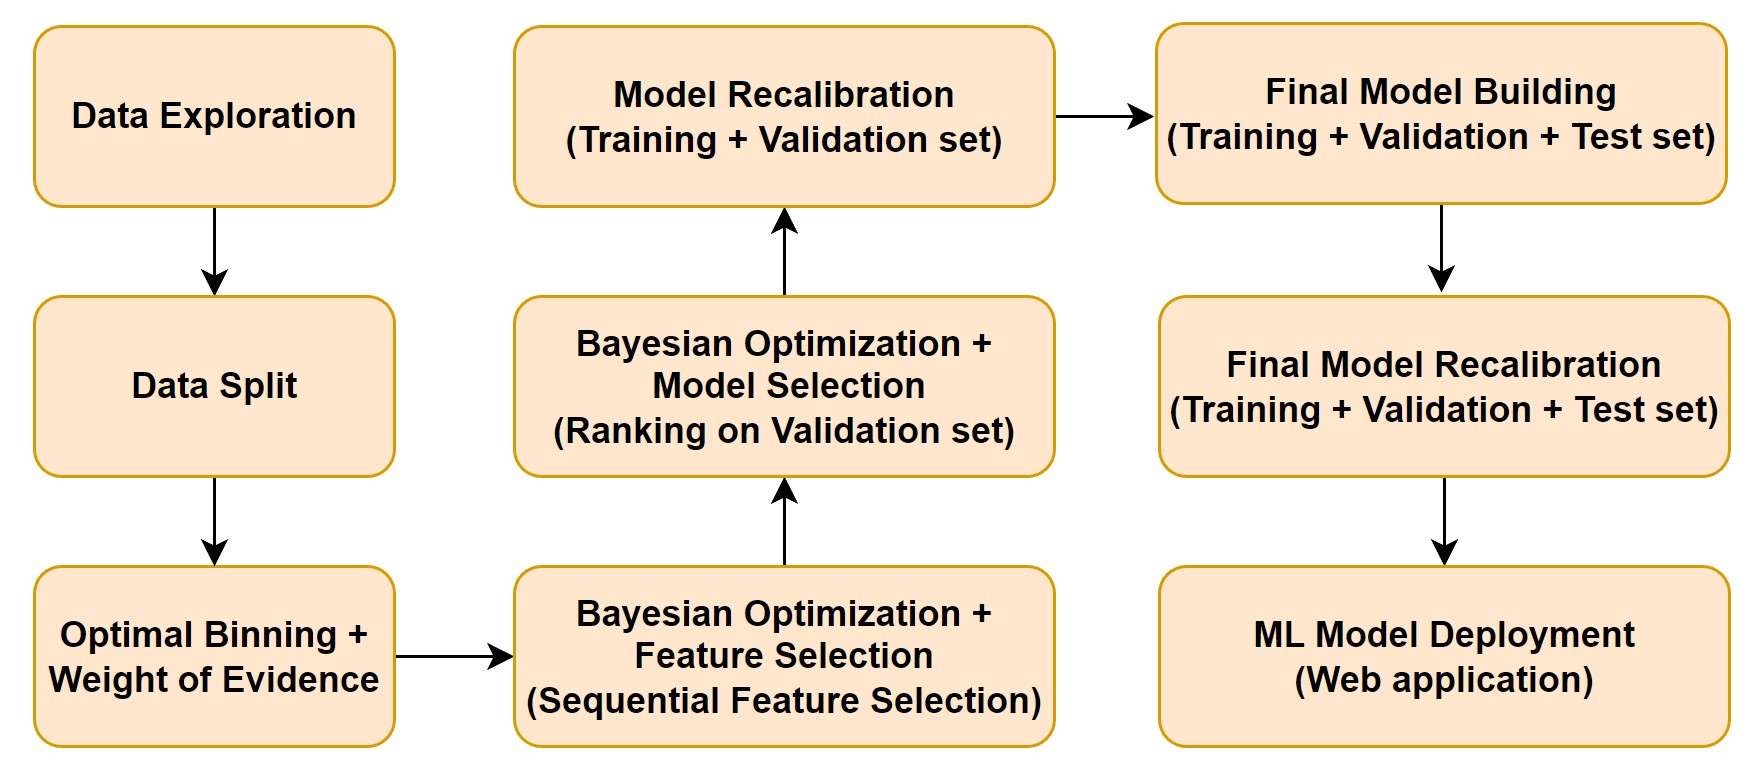
\includegraphics[width=120mm]{Figures/ml_framework.jpg}

\centering{\begin{source}Author's results\end{source}}\vspace{-1em}
\end{figure}

\newpage
\section{Repository and Environment Structure}

The whole machine learning implmenetation as the scope of this thesis is done mainly using Python Programming Language and further with collaboration of Git and HTML.
The whole repository can be found in the separate appendix or is available on the GitHub repository \url{https://github.com/petr-ngn/FFU_VSE_Masters_Thesis_ML_Credit_Risk_Modelling}.
The repository structure is shown in \autoref{fig:repostructure}.
\begin{figure}[H]
\centering\caption{Repository Structure}
\label{fig:repostructure}

{\footnotesize
\begin{verbatim}

            |--- data
            |  |--- interim_dat.csv
            |  |--- preprocessed_data.csv
            |  |--- raw_data.csv
            |
            |--- flask_app
            |  |--- inputs
            |  |  |--- inputs_flask_app_dict.pkl
            |  |
            |  |--- templates
            |  |  |--- index.html
            |  |  |--- results.html
            |  |
            |  |--- static
            |  |
            |  |--- app.py
            |
            |--- models
            |  |--- feature_preprocessing
            |  |--- feature_selection
            |  |--- model_selection
            |  |--- objects_FINAL
            |
            |--- plots
            |--- Masters_Thesis.ipynb
            |--- README.md
            |--- requirements.yml
\end{verbatim}
}
\centering{\begin{source}Author's results at GitHub\end{source}}\vspace{0em}
\end{figure}


\begin{itemize}\setlength\itemsep{0em}
\item \texttt{data} - directory containing the raw data, partially preprocessed data (\texttt{interim}) and the final preprocessed data.
\item \texttt{flask\_app} - directory containing the Flask application which is used for the deployment of the model. Particularly, it contains the \texttt{app.py} file which is the main back-end file of the application, the \texttt{templates} and \texttt{static} subdirectories which contain the front-end HTML files for the application, and the \texttt{inputs} subdirectory which contains the input dictionary for the application (such as the trained model, threshold, final features etc.).
\item \texttt{models} - directory containing the the subdirectories of the trained and fitted objects for features preprocessing, feature selection and model selection, including the final objects used in deployment.
\item \texttt{plots} - directory containing the plots generated within the main Python notebook.
\item \texttt{Masters\_Thesis.ipynb} - main Python notebook containing the main part of the machine learning Implementation, such as exploratory analysis, data preprocessing, training and evaluation of the models.
\item \texttt{README.md} - README file containing the description of the repository.
\item \texttt{requirements.yml} - file containing the list of the required packages and their specific versions used in this project.
\end{itemize}

This particular solution is developed in Python version 3.10.9 and these are the main packages and modules used in this project:
\begin{itemize}\setlength\itemsep{0em}
\item \lstinline{NumPy}, \lstinline{Pandas} - for data manipulation and analysis.
\item \lstinline{Matplotlib}, \lstinline{Seaborn} - for data visualization.
\item \lstinline{Scipy} - for statistical analysis.
\item \lstinline{OptBinning} - for optimal binning of features with respect to the target.
\item \lstinline{ImbLearn} - for handling imbalanced data using oversampling.
\item {Scikit-learn} - for feature selection, model selection and model evaluation.
\item {Scikit-optimize} - for more advanced hyperparameter optimization.
\item {Flask} - for deployment of the model as web application.
\end{itemize}

To replicate this solution, one may download this repository as a zip file or either can clone this repository using Git to the local repository. Before running any files or scripts, it is important to set the environment for such project using the file \texttt{requirements.yml}. This can be done by running the following command in the Anaconda terminal which will create the new environment with the name \texttt{FFU\_VSE\_Masters\_Thesis} and install all the required packages:
\begin{figure}[H]
\centering\
{\footnotesize
\begin{verbatim}
>> conda env create -n FFU_VSE_Masters_Thesis -f requirements.yml    
\end{verbatim}
\vspace{-1em}
}
\end{figure}
Be aware of your current path directory in your terminal. In order to install the file \texttt{requirements.yml}, you need to define a path to the directory, where such file is located.
To achieve this, the user has to either change the path in the terminal using \texttt{cd} command, insert the path directory before the \texttt{requirements.yml} in terminal, or to copy the file \texttt{requirements.yml} to the current path directory. The following code shows the former approach:
\begin{figure}[H]
\centering\
{\footnotesize
\begin{verbatim}
>> cd C:\Users\ngnpe\FFU_VSE_Masters_Thesis_ML_Credit_Risk_Modelling
>> conda env create -n FFU_VSE_Masters_Thesis -f requirements.yml   
\end{verbatim}
\vspace{-1em}
}
\end{figure}


To preserve the reproducibility of this solution and conistency of the results, the random seed is instantiated to \texttt{42}, so for instance data split, model optimization or training would be deterministic and not totally random everytime when replicating the solution.

Some \lstinline{Scikit-learn} or \lstinline{Scikit-optimize} objects have optional argument \texttt{n\_jobs} which utilizes the number of CPU cores used during the parallelizing computation. Such argument was set to \texttt{-1}, hence all the processors are used in order to  speed up the training or optimization process.

\newpage
\section{Data Exploration}
This section is focused on exploration of the analyzed loan data set, particularly on data set description, distribution analysis and association analysis, in order to infer potential valuable insights and hypotheses which can be used in the preprocessing or modelling part.

\subsection{Data Set Description}
The analyzed data set pertains to the HMEQ data set which contains loan application information and default status of 5,960 US home equity loans. Such data set was acquired from Credit Risk Analytics website\footnote{\url{http://www.creditriskanalytics.net/datasets-private2.html}} \citep{baesens2016credit}. Since this data set regards the loan application scoring data, using macroeconomic or other external data is omitted due to the data set characteristics as well as modelling with behavioral scoring.
Thus our goal is to predict whether the loan applicant will or would default based on provided information from the loan application.

As can be seen in \autoref{tab:data set}, the data set contains 13 columns, 12 features and 1 target variable \texttt{BAD} indicating whether the loan was in default (\texttt{1}) or not (\texttt{0}). 
Amongst the 12 features, there are 10 numeric features and 2 categorical features, namely \texttt{REASON} which contains 2 categories - Debt consolidation (\texttt{DebtCon}) and Home improvement (\texttt{HomeImp}), and \texttt{JOB} which fontains following categories - Administration (\texttt{Office}), Sales, Manager (\texttt{Mgr}), Professional Executive (\texttt{ProfExe}), Self-employed (\texttt{Self}), and Other.


\begin{table}[H]
\small
\setlength{\tabcolsep}{8pt}
\renewcommand{\arraystretch}{1.3}
\begin{center}
\caption[Data Set Columns]{Data Set Columns}\label{tab:dataset}
\begin{tabular}{@{} l p{8cm} l @{}}
\toprule
\textbf{Variable} & \textbf{Description} & \textbf{Data type}\\
\midrule
\hline
BAD & Default status & Boolean \\

LOAN & Requested loan amount & numeric \\

MORTDUE & Loan amount due on existing mortgage & numeric \\

VALUE & Value of current underlying collateral property & numeric \\

REASON & Reason of loan application & categorical \\
JOB & Job occupancy category & categorical \\

YOJ & Years of employment at present job & numeric \\

DEROG & Number of derogatory public reports & numeric \\

DELINQ & Number of delinquent credit lines & numeric \\

CLAGE & Age of the oldest credit line in months & numeric \\

NINQ & Number of recent credit inquiries & numeric \\

CLNO & Number of credit lines & numeric \\

DEBTINC & Debt-to-income ratio & numeric \\
\hline
\bottomrule
\end{tabular}
\end{center}
\begin{center} % Center the source
\source{\citep{baesens2016credit}}
\end{center}
\end{table}

After the initial data inspection, data does not contain any duplicates but does contain missing values, which are summarized in \autoref{tab:natable}.
Most of the missing values contains the feature \texttt{DEBTINC} with 1,267 missing observations, whereas columns indicating default status (\texttt{BAD}) or requested loan amount (\texttt{LOAN}) do not contain any missing values, which is expected as the bank should have the available information about their loans whether they have defaulted or not, and since this data set pertains to the application scoring, when applying for a loan, an applicant should always fill out the requested loan amount.

\begin{table}[H]
\small
\setlength{\tabcolsep}{8pt}
\renewcommand{\arraystretch}{1.3}
\centering
\caption[Missing Values Summary]{Missing Values Summary}\label{tab:natable}
\begin{tabular}{l r r}
\toprule
\textbf{Columns} & \textbf{\# NA's} & \textbf{\% NA's}\\
\midrule
\hline
BAD & 0 & 0.00 \% \\
LOAN & 0 & 0.00 \% \\
MORTDUE & 518 & 8.69 \% \\
VALUE & 112 & 1.88 \% \\
REASON & 252 & 4.23 \% \\
JOB & 279 & 4.68 \% \\
YOJ & 515 & 8.64 \% \\
DEROG & 708 & 11.88 \% \\
DELINQ & 580 & 9.73 \% \\
CLAGE & 308 & 5.17 \% \\
NINQ & 510 & 8.56 \% \\
CLNO & 222 & 3.72 \% \\
DEBTINC & 1267 & 21.26 \% \\
\hline
\bottomrule
\end{tabular}
\vspace{0.35em}

\centering{\begin{source}Author's results in Python\end{source}}\vspace{-1em}
\end{table}


\subsection{Distribution Analysis}
\label{subsec:distribution}
In this subsection, we inspect the distribution of our variables, including the target variable and the features.
Such distribution inspection may help us to identify potential outliers, missing values, and other potential issues with the data set.

\subsubsection{Default Distribution}

Regarding the the target variable distribution, from the \autoref{fig:defaultdist} we can observe that the default status distribution is heavily imbalanced, as most of the loans have not defaulted yet.
Particularly, 80.05\% of the observations have been labelled as non-default (4,771 observations) and 19.95\% observations labelled as default (1,189 observations).
This may cause problems in the modelling part, as the model may be biased towards the majority class, i.e., the non-default class. Such imbalanced class issue will be further treated in \autoref{subsec:data-split-ADASYN}.

\begin{figure}[H]
\centering
\caption{Default status distribution}
\label{fig:defaultdist}
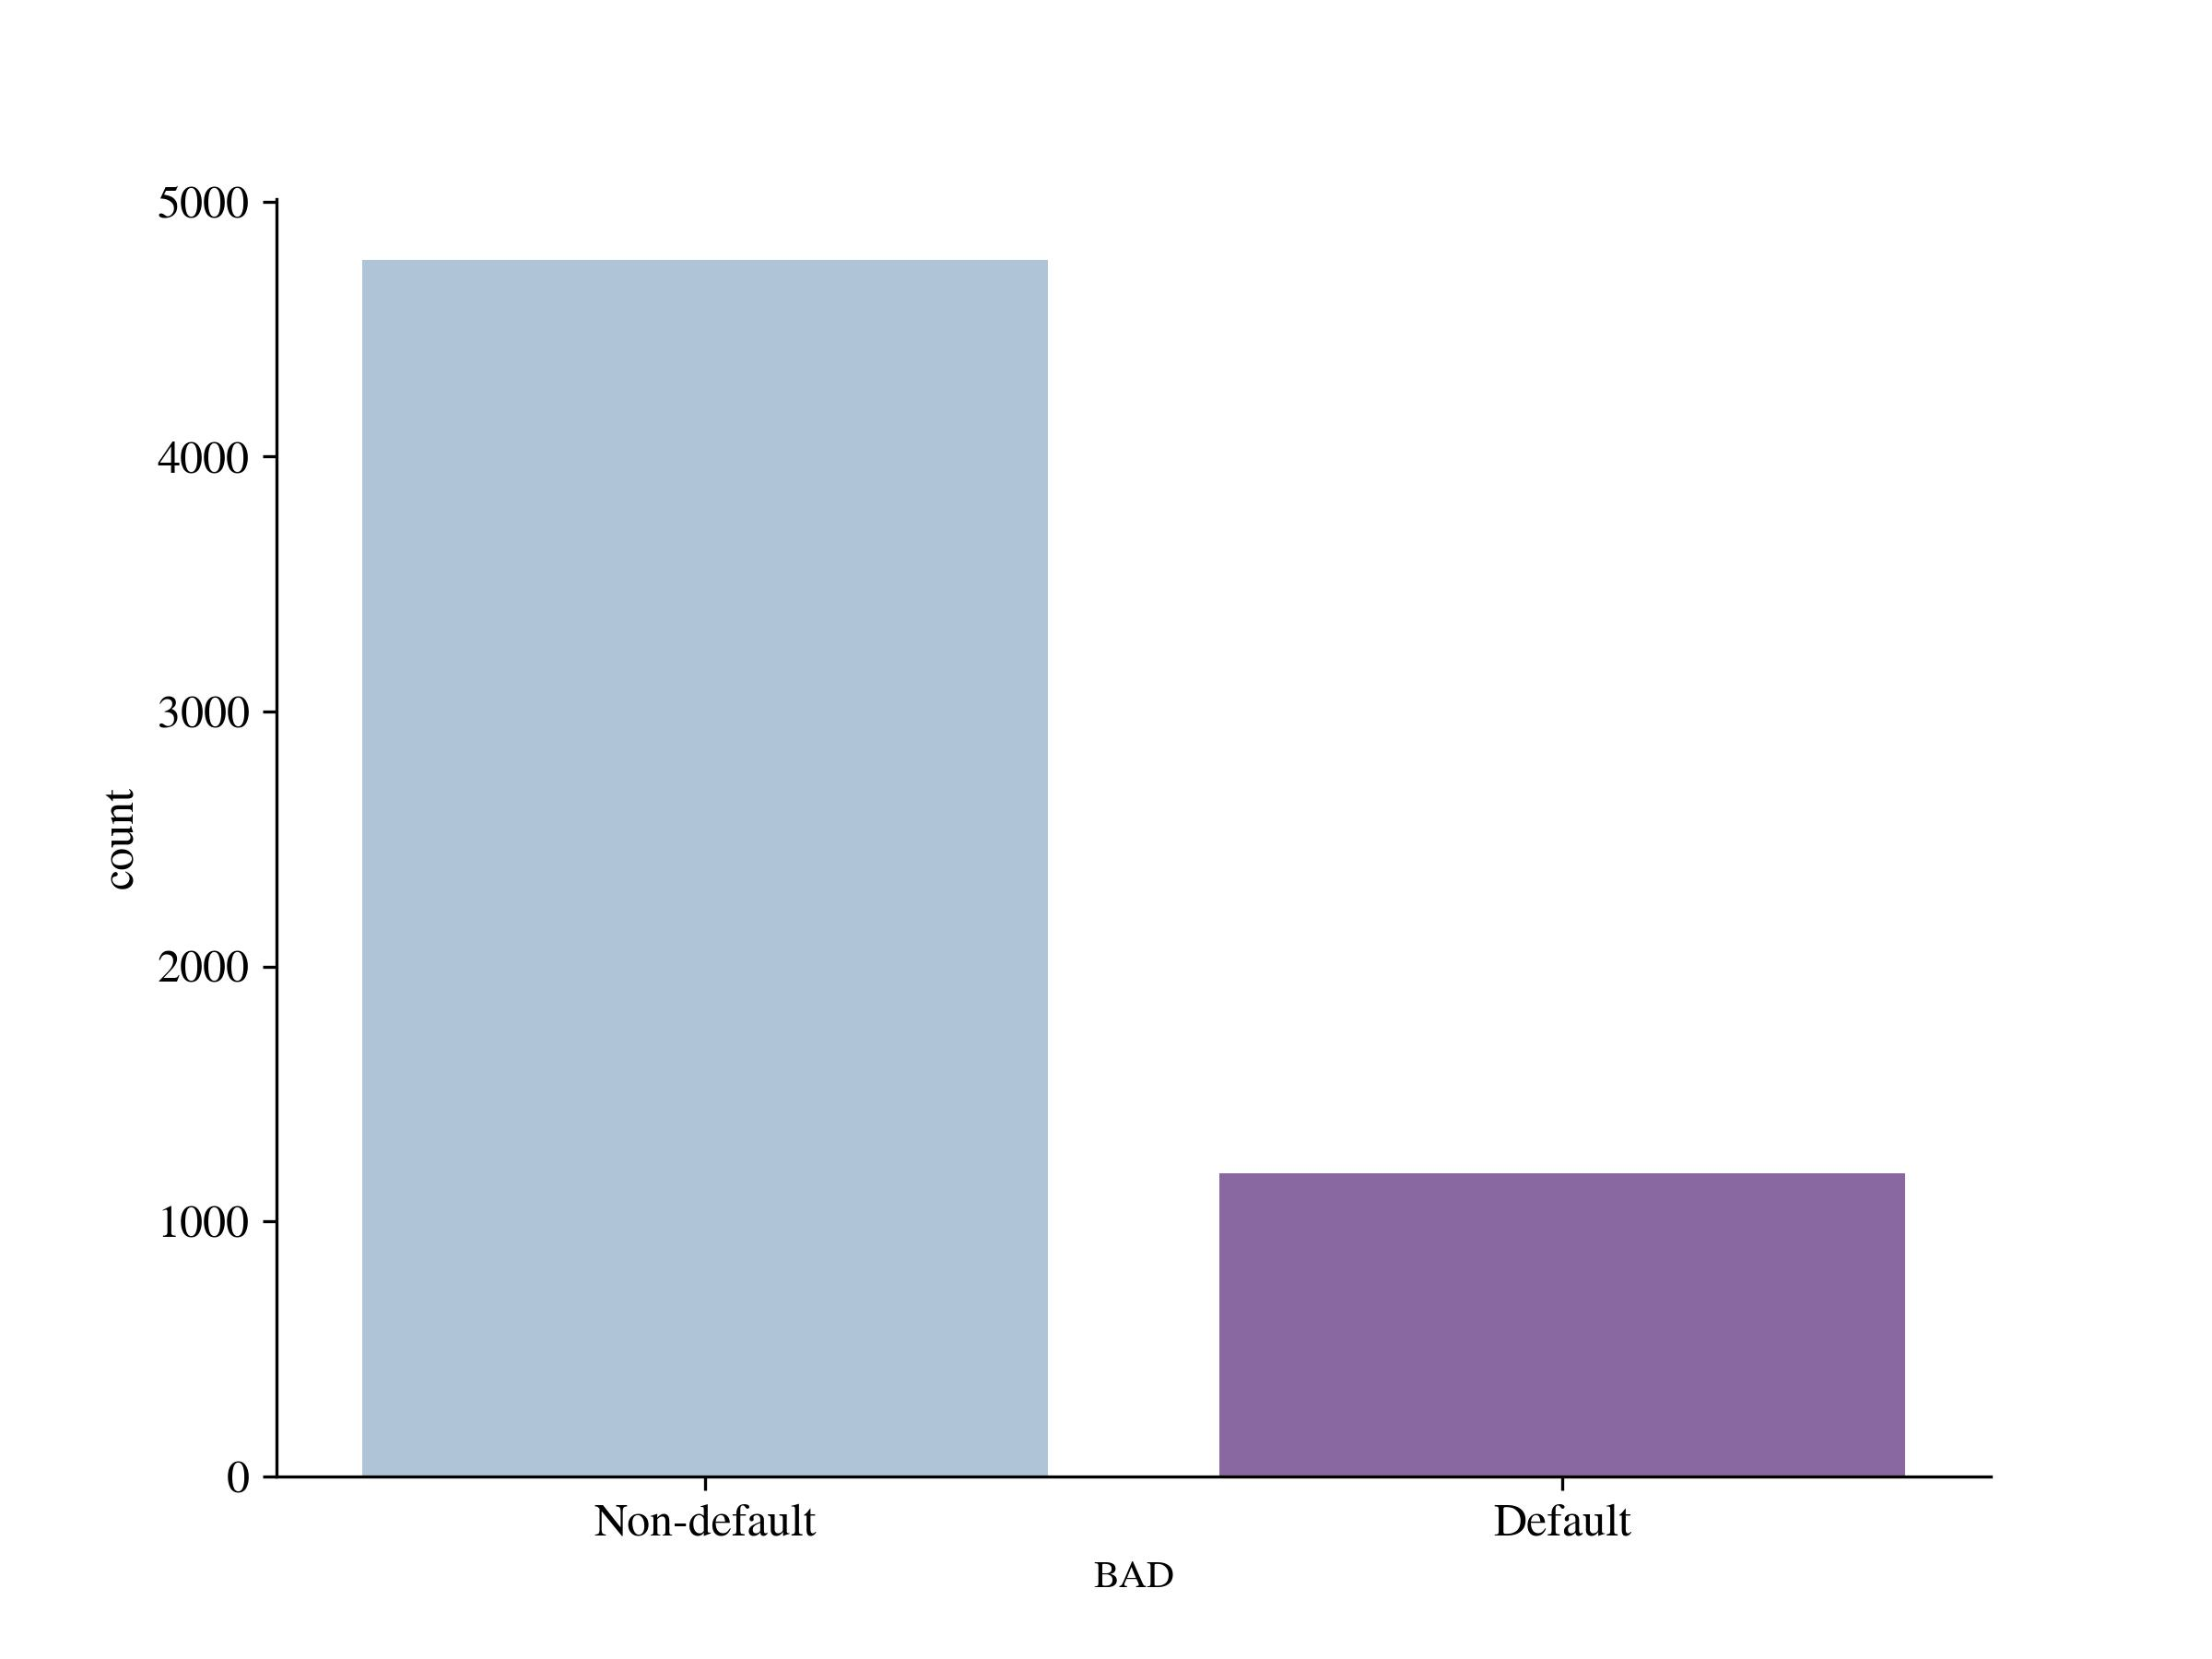
\includegraphics[width=130mm]{Figures/Default_Distribution.jpg}\vspace{-1em}
\centering{\begin{source}Author's results in Python\end{source}}\vspace{-1em}
\end{figure}

\subsubsection{Numeric Features' Distribution}
\label{subsubsec:numdist}

Regarding the numeric features, it can be observed that most of them exhibit a positive skewness and contain outliers, as illustrated in \autoref{fig:boxfeat}, which depicts the conditional distribution of the numeric features with respect to the default status via boxplots.

All the outliers appear to be valid, indicating that they have not arisen due to data entry errors.
This can be attributed to the non-negative nature of all the numeric features, which makes it impossible to have negative values for features such as the number of years at present job or the number of delinquent credit lines, among others.
Additionally, the maximum values of the given features are not unrealistically high, further corroborating the validity of the outliers.
However, it is necessary to treat these outliers as they can bias a model's weights or coefficients, particularly in the case of logistic regression or neural networks.
Outliers can also jeopardize distance calculations in the case of KNN, or in general, affect the position and orientation of the decision boundary.
Such factors can lead to overfitting and inaccurate and biased predictions.
A detailed explanation of the outlier treatment is provided in \autoref{subsec:prep-optbinning}.

Concerning the target variable, it can be observed that there are some differences in the distribution shapes of \texttt{DEROG} and \texttt{DELINQ}, which exhibit less skewness and lower dispersion for non-default cases as compared to default cases.
Since both features indicate negative information about delinquency, it is expected that a higher value for these features would increase the likelihood of loan default.
Referring to the feature \texttt{DEBTINC}, it does not exhibit any extreme values for non-default cases, but some extreme values are present for default cases.
From this, it can be inferred that if the debt-to-income ratio is too high, indicating that the applicant's income is not sufficient to cover their debt, the loan is more likely to end in default.
The association between the default status and the numeric features is further investigated in \autoref{subsubsec:target-num-ass}.

\begin{figure}[H]
\centering
\caption{Conditional distribution of numeric features}\vspace{0.5em}
\label{fig:boxfeat}
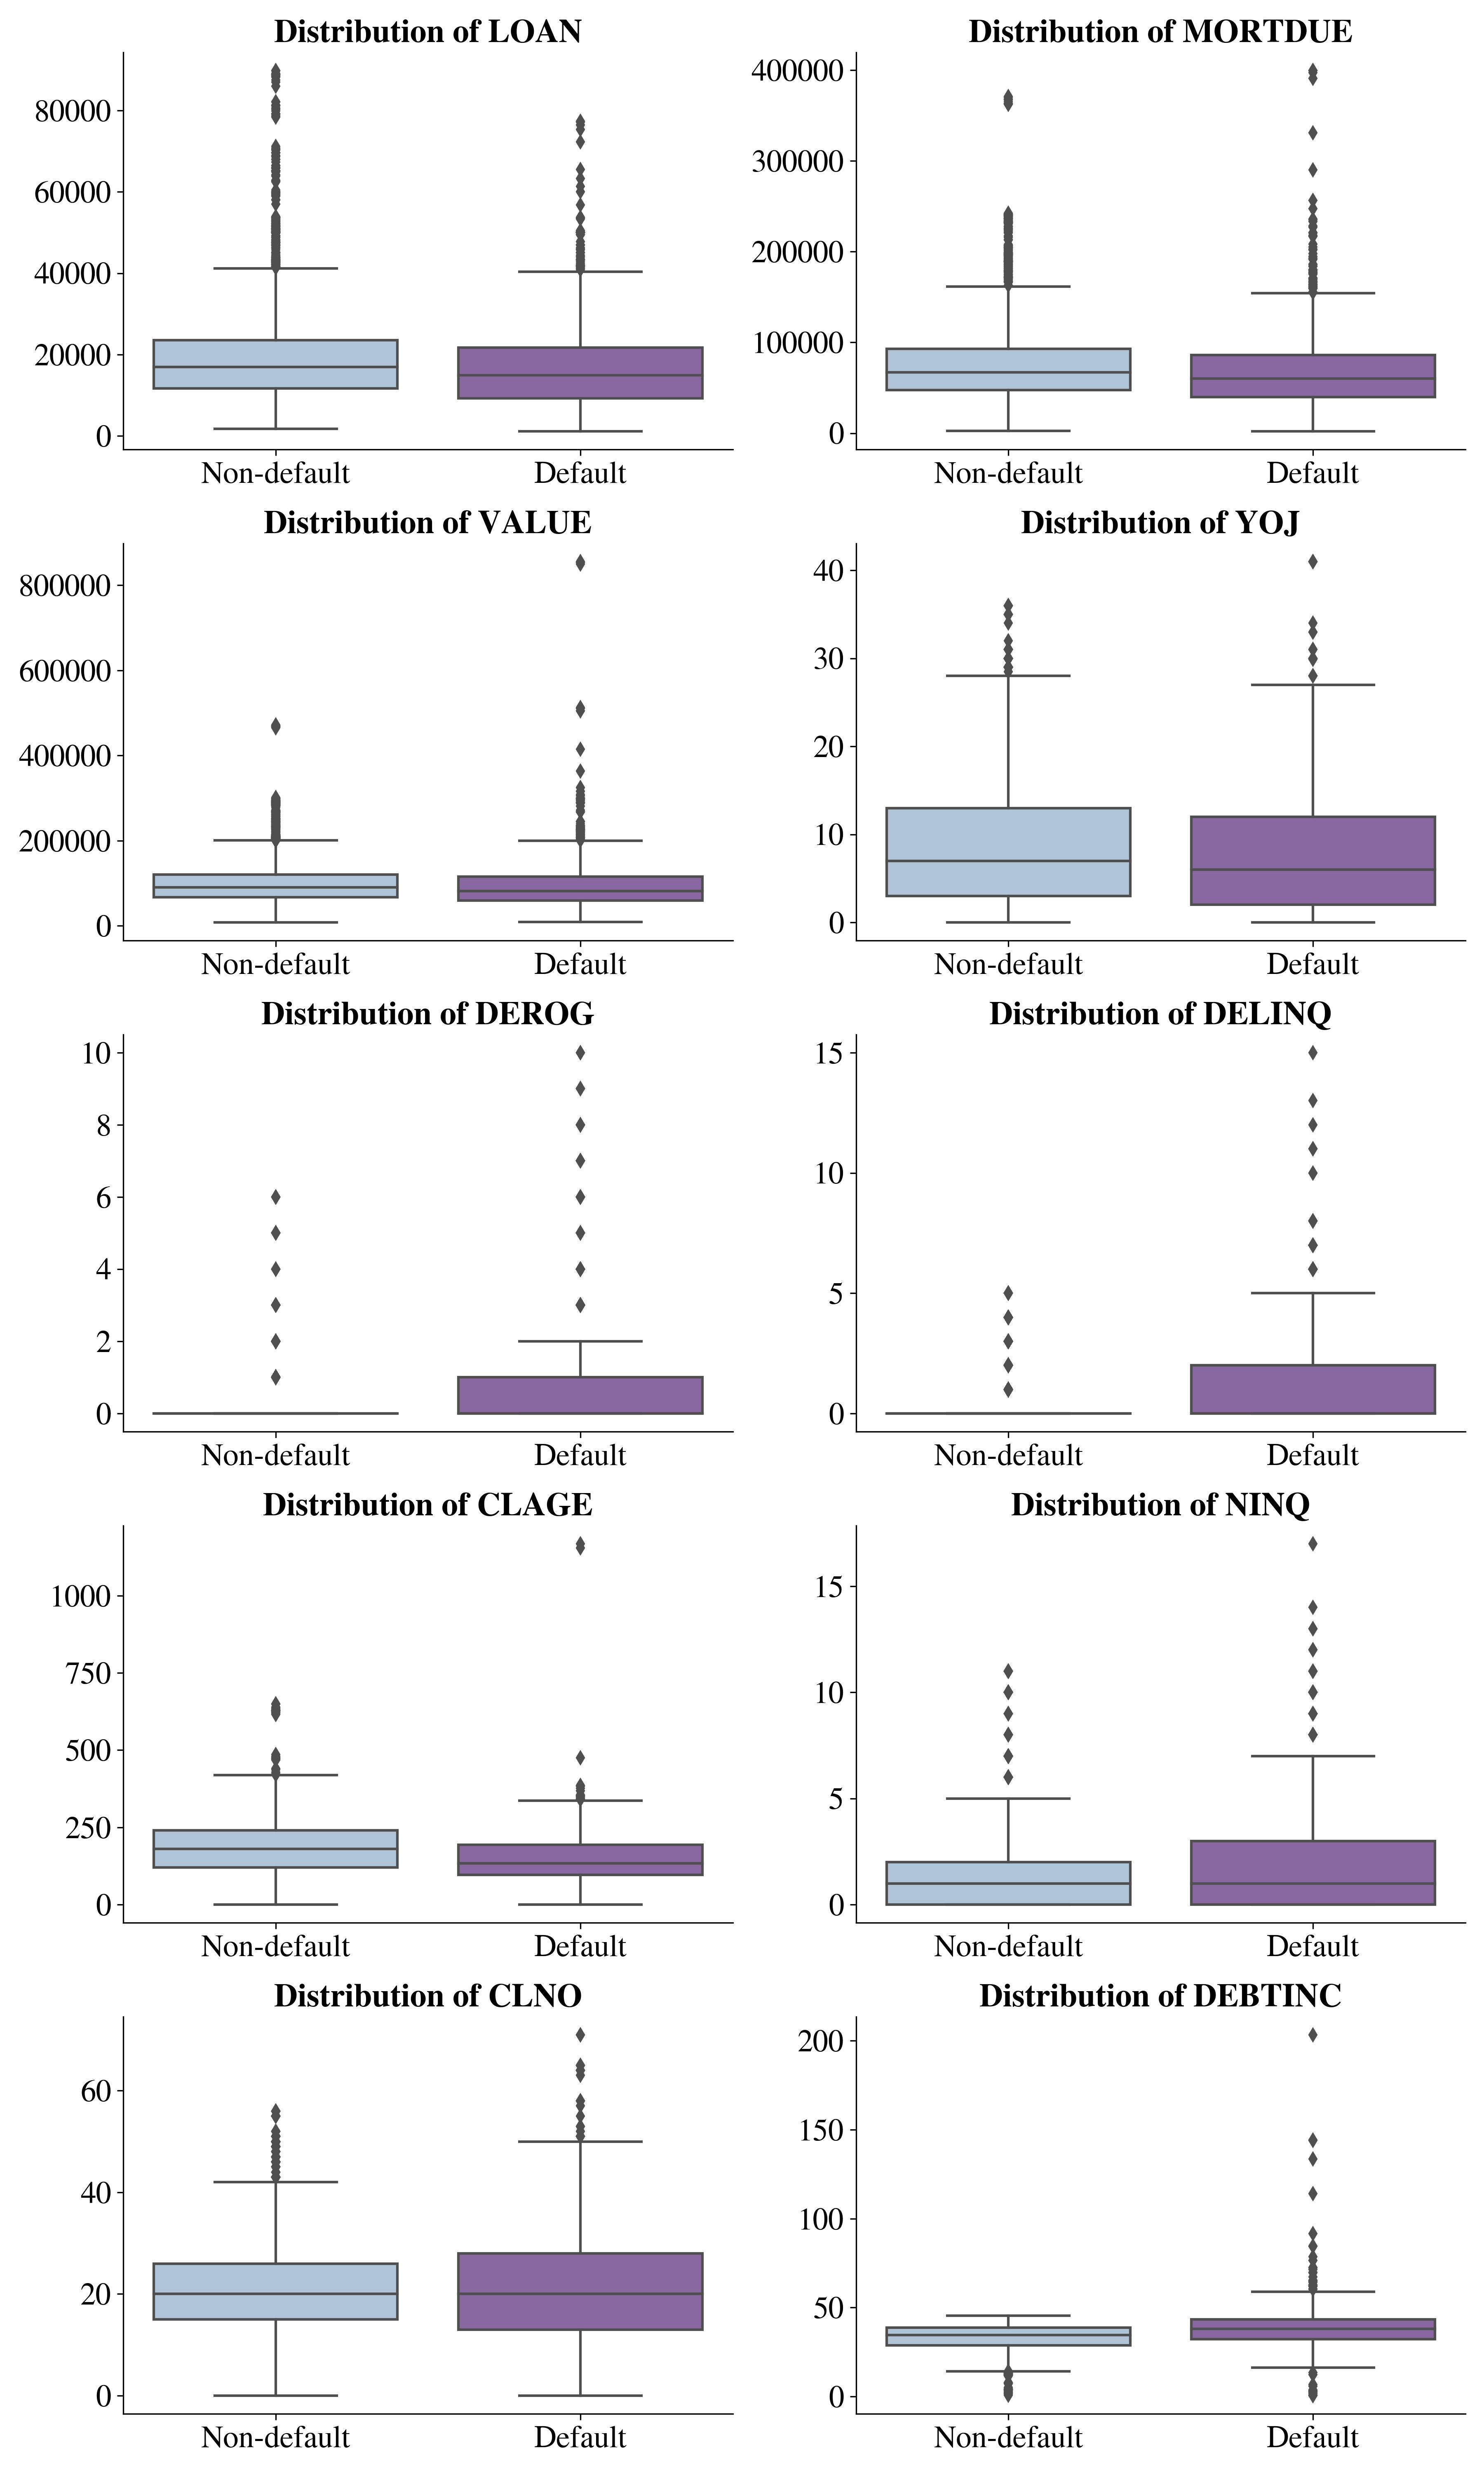
\includegraphics[width=140mm]{Figures/Numeric_Features_Distribution_Boxplots.jpg}
\centering{\begin{source}Author's results in Python\end{source}}\vspace{-1em}
\end{figure}

Due to the fact that the boxplots do not capture the missing values occurred in given features, it is also important to inspect the numbers and proportions of missing values in each feature, conditional on the default status.
As can be seen in \autoref{tab:nacont-table}, $n_0$ refers to the number of missing values in given feature for non-default cases, $n_1$ refers to the number of missing values in given feature for default cases.
$N_0$ and $N_1$ refer to the total number non--default cases and default cases respectively, therefore $n_0/N_0$ refers to the proportion of missing values in given feature for non-default cases, and $n_1/N_1$ refers to the proportion of missing values in given feature for default cases.

Pertaining to the feature \texttt{DEBTINC}, we can observe a significant difference in the number of missing values between the default and non-default cases. Out of all defaulted loans, 66.11 \% had missing debt--to--income ratio, whereas only 10.08 \% out of all non-defaulted loans had missing debt--to--income ratio.
Therefore, there could be a strong association between the missing debt--to--income ratio and the default.

Similarly, the table depicts a significant difference with respect to \texttt{VALUE} as 0.15 \% had missing collateral property value out of all non--defaulted loan, and 8.92 \% defaulted loans had missing collateral property value.
It can be inferred that loan applicants who withhold information on their collateral property value or debt-to-income ratio are more likely to default on their loans.
This may be due to negative information that they are trying to conceal, such as an excessively high debt or low income, or a low collateral property value.
Such associations are further investigated in \autoref{subsubsec:target-na-ass}.


\begin{table}[H]
\small
\setlength{\tabcolsep}{8pt}
\renewcommand{\arraystretch}{1.3}
% define a new column type 'L' for left alignment
\newcolumntype{R}[1]{>{\raggedleft\arraybackslash}p{#1}} % define a new column type 'R' for right alignment
\begin{center}
\caption[Numeric features NA's table]{Numeric features NA's table}\label{tab:nacont-table}
\begin{tabular}{l R{1cm}R{1cm}|R{1.5cm}R{1.5cm}}
    \toprule
    \textbf{Feature} & \textbf{$n_0$} & \textbf{$n_1$} & \textbf{$n_0/N_0$} & \textbf{$n_1/N_1$} \\
    \midrule
    \hline
    LOAN & 0 & 0 & 0 \% & 0 \% \\

    MORTDUE & 412 & 106 & 8.64 \% & 8.92 \% \\

    VALUE & 7 & 105 & 0.15 \% & 8.83 \% \\

    YOJ & 450 & 65 & 9.43 \% & 5.47 \% \\

    DEROG & 621 & 87 & 13.02 \% & 7.32 \% \\

    DELINQ & 508 & 72 & 10.65 \% & 6.06 \% \\

    CLAGE & 230 & 78 & 4.82 \% & 6.56 \% \\

    NINQ & 435 & 75 & 9.12 \% & 6.31 \% \\

    CLNO & 169 & 53 & 3.54 \% & 4.46 \% \\

    DEBTINC & 481 & 786 & 10.08 \% & 66.11 \% \\ \hline
    \bottomrule
\end{tabular}
\end{center}
\begin{center}
\source{Author's results in Python}
\end{center}
\end{table}
\subsubsection{Categorical Features' Distribution}
\label{subsubsec:catdist}

Regarding the distribution of categorical features, the data set includes 2 nominal features, namely \texttt{REASON} and \texttt{JOB}.
The conditional distribution of categorical features on the default status is visualized using barplots in \autoref{fig:catdist}.
The plot indicates that most loan applicants applied for debt consolidation, while most job occupancies were labeled as \texttt{Other}.

With respect to the default status, there appears to be no significant difference between the default and non-default cases in terms of the relative distribution of the \texttt{REASON} feature.
However, a slight difference is observed between the default and non-default cases in terms of the relative distribution of the \texttt{JOB} feature.
Specifically, the categories \texttt{Office}, \texttt{ProfExe}, and \texttt{N/A} exhibit a relatively higher proportion of non-default cases than default cases.
Hence, a moderate association between the \texttt{JOB} feature and the default status is possible, as further investigated in \autoref{subsubsec:target-cat-ass}.


\begin{figure}[H]
\centering
\caption{Conditional distribution of categorical features}\vspace{0.5em}
\label{fig:catdist}
\includegraphics[width=140mm]{Figures/Categorical_Features_Distribution.jpg}
\centering{\begin{source}Author's results in Python\end{source}}\vspace{-1em}
\end{figure}
\subsection{Association Analysis}
In this subsection, we aim to examine potential relationships between the variables by analyzing their associations. Firstly, we investigate the association between the default status and the features. Subsequently, we explore the association among the features themselves.

\subsubsection{Association between default status and numeric features}
\label{subsubsec:target-num-ass}

To measure the association between the target variable and the numeric features, we use the Point-Biserial correlation coefficient, which is the Pearson's product moment correlation coefficient between a continuous variable and a dichotomous variable \citep{kornbrot2014point}.
This coefficient ranges from -1 to +1 and can be used to assess the strength and direction of the relationship between a continuous variable and a binary variable.
The formula for computing this coefficient is as follows:

\begin{equation}\label{eq}
r_{pb,X} =  \frac{\mu \left( X | Y=1 \right) -\mu \left( X | Y=0 \right)}{\sigma_{X}}\sqrt{\frac{N\left(Y=1\right) \times N\left(Y=0\right)}{N \left(N - 1 \right)}}
\end{equation}

Here, $\mu \left( X | Y=1 \right)$ and $\mu \left( X | Y=0 \right)$ represent the means of the given numeric feature $X$ conditional on the default status and non-default status, respectively, while $\sigma_{X}$ denotes the standard deviation of $X$.
The values of $N\left(Y=1\right)$ and $N\left(Y=0\right)$ indicate the number of observations with default status and non-default status, respectively, and $N$ represents the total number of observations within the feature $X$.


The following \autoref{tab:pointbi} displays the computed Point-Biserial coefficient for each numeric feature with respect to the default status, along with its statistical significance.
The results show that features such as \texttt{DEROG}, \texttt{DELINQ}, and \texttt{DEBTINC} are moderately and positively associated with the default status at the 1\% statistical significance level.
These findings support the observations made in \autoref{subsubsec:numdist} regarding the positive associations of these features with the default status. It can be inferred that these features may serve as important predictors in the model.

\begin{table}[H]
    \small
    \setlength{\tabcolsep}{8pt}
    \renewcommand{\arraystretch}{1.3}
    \centering
        \caption[Point--Biserial Correlation table]{Point--Biserial Correlation table}\label{tab:pointbi}
        \begin{tabular}{@{} l r @{\hspace{1cm}} l @{}}
    \toprule
    \textbf{Feature} & \textbf{Coefficient} & \textbf{Significance}\\
    \midrule
    \hline

    LOAN & -0.075  & ***\\

    MORTDUE & -0.048  & ***\\

    VALUE & -0.030  & ** \\
    
    YOJ & -0.060  & *** \\

    DEROG & 0.276 & *** \\

    DELINQ & 0.354 & *** \\
    
    CLAGE & -0.170 & *** \\

    NINQ & 0.175 & *** \\

    CLNO & -0.004 & \\

    DEBTINC & 0.200 & *** \\
    \hline
    \bottomrule
    \end{tabular}
    \vspace{0.35em}


        \centering\footnotesize{$^{*}$: $p<0.10$, $^{**}$: $p<0.05$, $^{***}$: $p<0.01$}\vspace{0.7em}

        \centering{\begin{source}Author's results in Python\end{source}}\vspace{-1em}

\end{table}

\subsubsection{Association between default status and categorical features}
\label{subsubsec:target-cat-ass}

In order to measure the strength of the relationship between the dichotomous default status and categorical variables, we employ Cramer's V, which ranges from 0 to 1 and is defined as:


\begin{equation}\label{eq}
    CV_{X} = \sqrt{\frac{\chi^{2}}{N\left(k-1\right)}}
\end{equation}


As noted in \autoref{subsubsec:catdist}, the association between the default status and \texttt{REASON} is weak, as evidenced by the Cramer's V value being close to zero.
Conversely, the association between the default status and \texttt{JOB} is slightly stronger, as the categories \texttt{Office}, \texttt{ProfExe}, and \texttt{N/A} exhibit a higher proportion of non-default cases than default cases.
Both \texttt{REASON}'s and \texttt{JOB}'s associations with default status are statistically significant at the 1\% significance level.

While statistical significance is important, it does not necessarily indicate that a feature is a strong predictor of the target variable.
Ultimately, the usefulness of a feature in predicting the target variable is determined by the performance metrics of the model.

    \begin{table}[H]
        \small
        \setlength{\tabcolsep}{8pt}
        \renewcommand{\arraystretch}{1.3}
        \centering
            \caption[Cramer's V Association table]{Cramer's V Association table}\label{tab:cramer-v}
            \begin{tabular}{@{} l r @{\hspace{1cm}} l @{}}
        \toprule
        \textbf{Feature} & \textbf{Coefficient} & \textbf{Significance}\\
        \midrule
        \hline
        REASON & 0.038  & ***\\
        JOB & 0.120  & ***\\
        \hline

        \bottomrule
    \end{tabular}
    \vspace{0.35em}


        \centering\footnotesize{$^{*}$: $p<0.10$, $^{**}$: $p<0.05$, $^{***}$: $p<0.01$}\vspace{0.7em}

        \centering{\begin{source}Author's results in Python\end{source}}\vspace{-1em}
\end{table}

\subsubsection{Association between default status and missing values}
\label{subsubsec:target-na-ass}

Given that the loan data set contains missing values, it is necessary to examine whether the missingness is associated with the default status. One possible approach is to encode the feature with missing values as a binary variable, where 1 indicates the presence of a missing value and 0 otherwise.

To quantify the strength of association between the two binary variables, the Phi coefficient is used, which is defined as:

\begin{equation}\label{eq}
\phi_{X} = \sqrt{\frac{\chi^{2}}{n}}
\end{equation}

In line with the finding regarding the \texttt{DEBTINC} and \texttt{VALUE} in \autoref{subsubsec:numdist}, there is a strong and statistically significant association between the missing debt-to-income ratio and default status, and a moderate and statistically significant association between the missing collateral property value and default status, as shown in \autoref{tab:phi-target}.
Therefore, we can anticipate that these features will be crucial indicators in default prediction. Further details on feature selection are presented in \autoref{subsec:feature-selection}.
\begin{table}[H]
    \small
    \setlength{\tabcolsep}{8pt}
    \renewcommand{\arraystretch}{1.3}
    \centering
        \caption[Phi Correlation Coefficient table]{Phi Correlation Coefficient table}\label{tab:phi-target}
        \begin{tabular}{@{} l r @{\hspace{1cm}} l @{}}
    \toprule
    \textbf{Feature} & \textbf{Coefficient} & \textbf{Significance}\\
    \midrule
    \hline
    LOAN & 0.000  & \\
    \hline
    MORTDUE & 0.003  & \\
    \hline
    VALUE & 0.254  & *** \\
    \hline
    REASON & 0.004 & \\
    \hline
    JOB & 0.064 & *** \\
    \hline
    YOJ & 0.056  & *** \\
    \hline
    DEROG & 0.070 & *** \\
    \hline
    DELINQ & 0.061 & *** \\
    \hline
    CLAGE & 0.030 & ** \\
    \hline
    NINQ & 0.039 & *** \\
    \hline
    CLNO & 0.018 & \\
    \hline
    DEBTINC & 0.547 & *** \\
    \bottomrule
    \end{tabular}
    \vspace{0.35em}


        \centering\footnotesize{$^{*}$: $p<0.10$, $^{**}$: $p<0.05$, $^{***}$: $p<0.01$}\vspace{0.7em}

        \centering{\begin{source}Author's results in Python\end{source}}\vspace{-1em}
\end{table}

\subsubsection{Missing Values Association}
Additionally, it is imperative to investigate the relationship between missing values and default status, as well as the interrelationship between the missing values themselves.
A common approach to identifying patterns of missing data in a data set is through the use of a dendrogram, which clusters variables hierarchically based on the occurrence of missing values.
This method groups variables into clusters based on the similarity of their missing value patterns, such that variables with comparable patterns of missingness are clustered together.
Conversely, variables with dissimilar patterns of missingness are placed in separate clusters.
The dendrogram is constructed by merging the two closest clusters iteratively until all variables are in the same cluster.
The distance between the clusters at each step of the merging process is shown on the y-axis of the dendrogram, and the order in which the variables are merged is displayed on the x-axis.

In \autoref{fig:dendrogram}, the hierarchical clustering of the data set's variables is illustrated, excluding the default status and requested loan amount feature \texttt{LOAN}, as these variables do not contain any missing values.
As depicted in the dendrogram, the \texttt{CLNO} and \texttt{CLAGE} features have the most similar patterns of missing values occurrences.
Therefore, it can be inferred that a significant number of loan applicants tend to omit information regarding their number of credit lines (\texttt{CLNO}) and the age of their most recent credit line (\texttt{CLAGE}) when submitting their loan applications.

\begin{figure}[H]
    \centering
    \caption{Nullity dendrogram}\vspace{0.5em}
    \label{fig:dendrogram}
    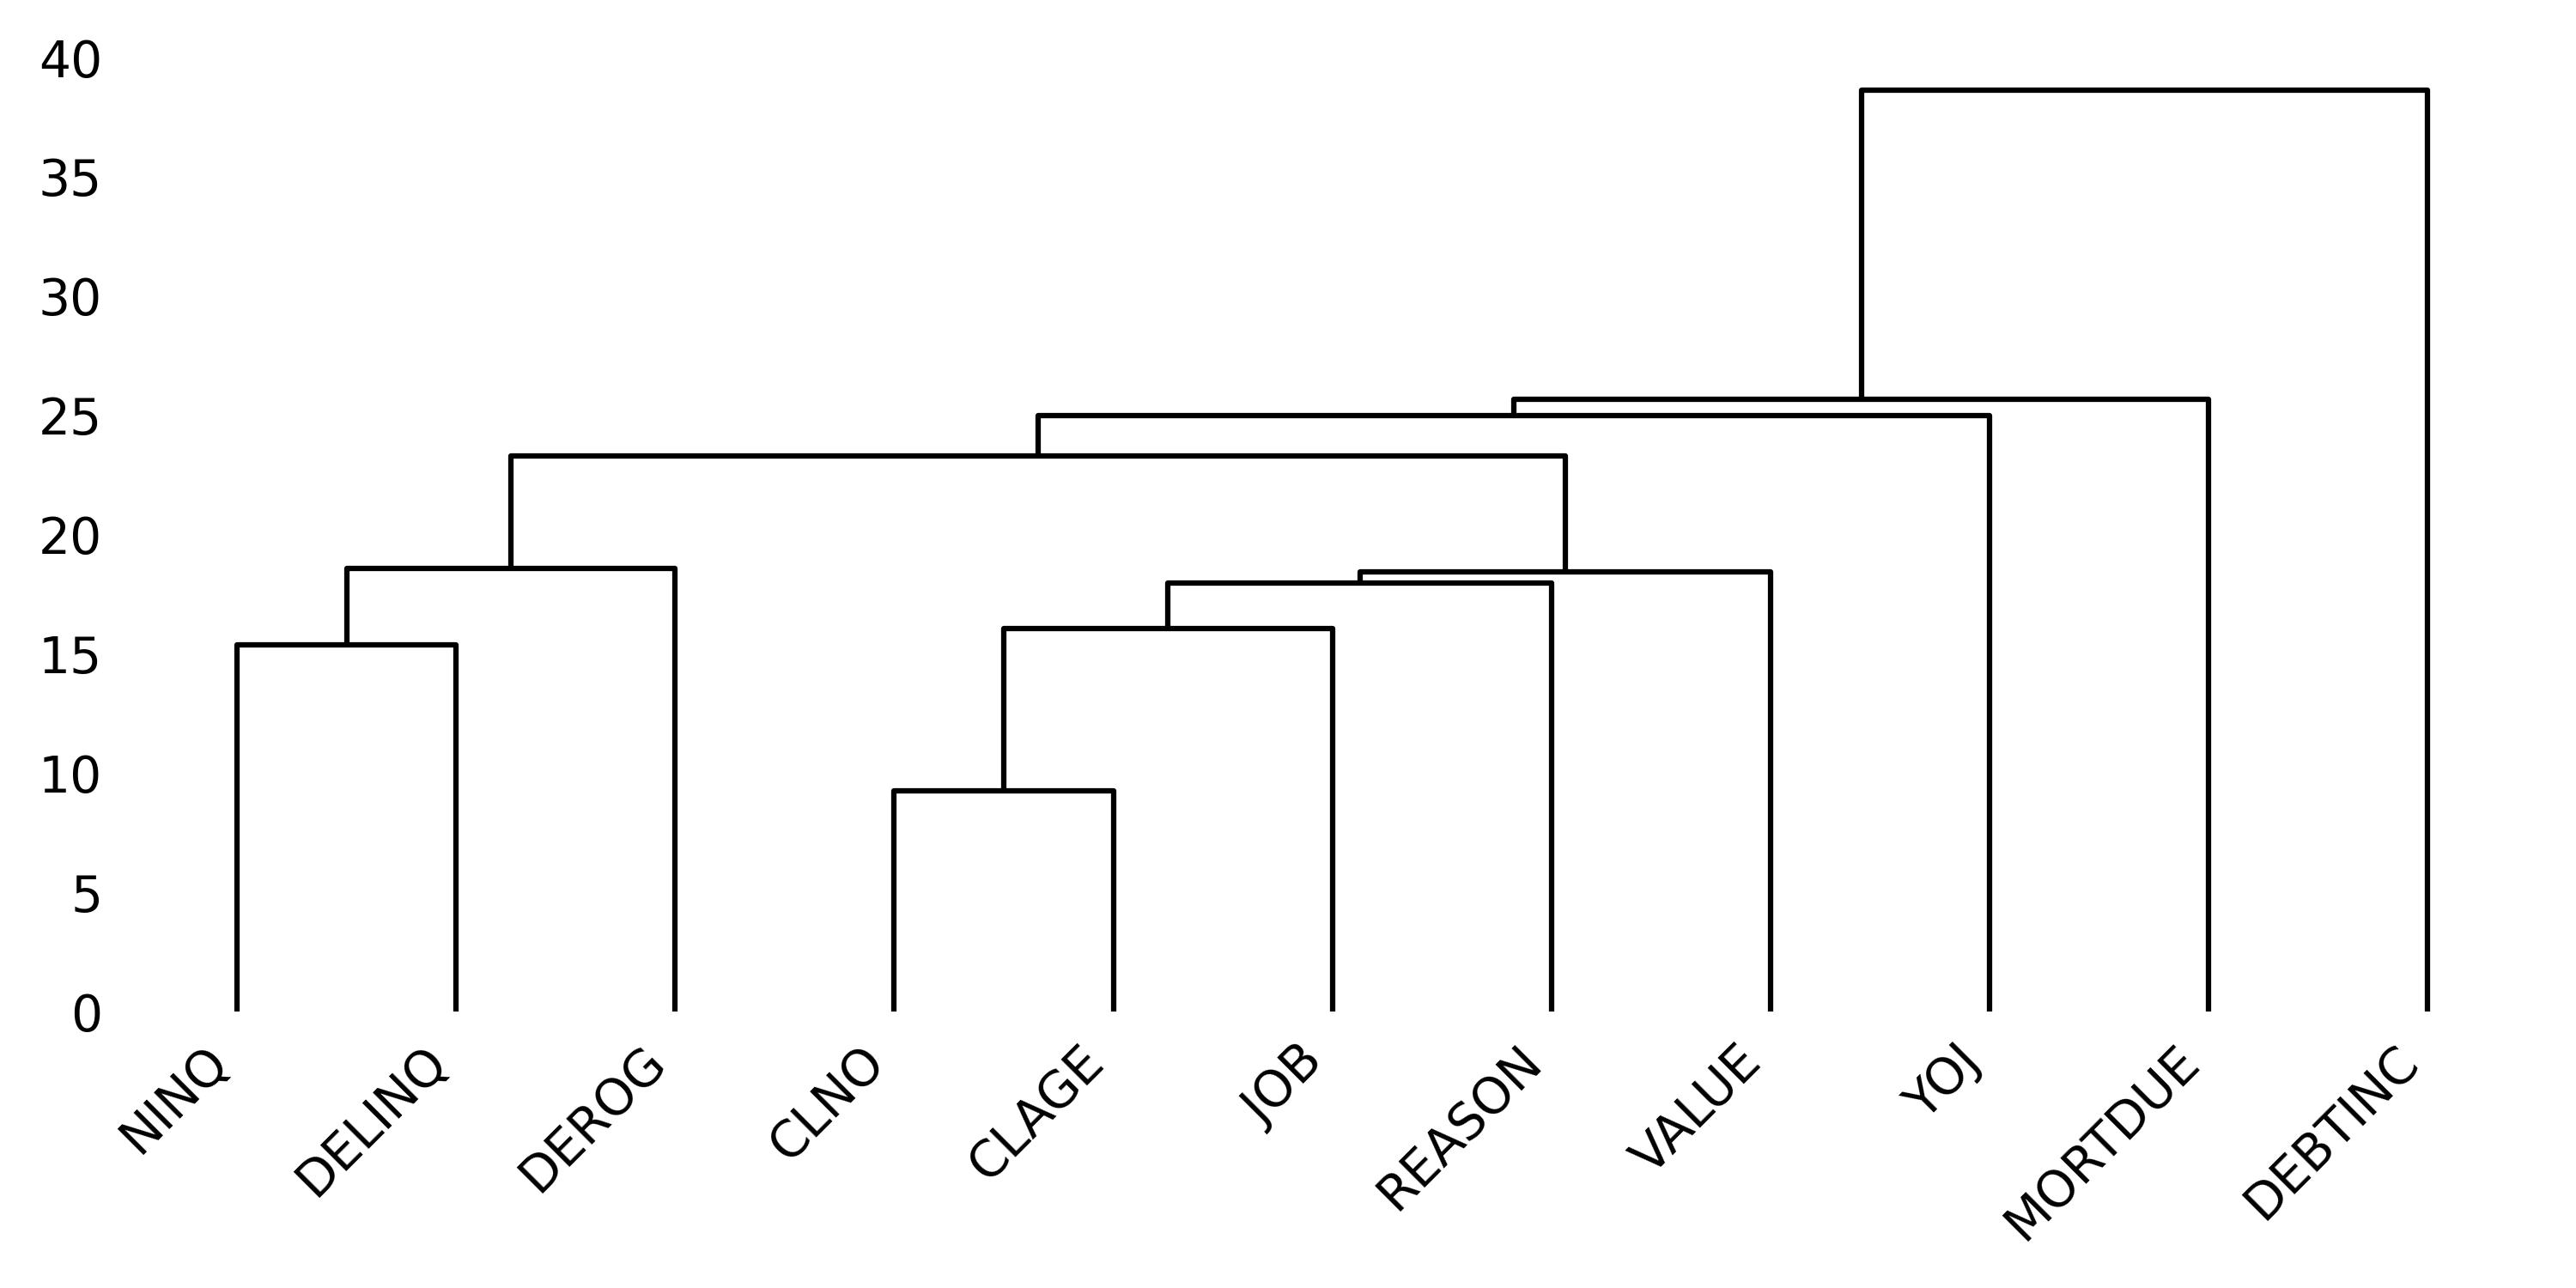
\includegraphics[width=140mm]{Figures/NA_Dendrogram.jpg}
    \centering{\begin{source}Author's results in Python\end{source}}\vspace{-1em}
\end{figure}

\subsubsection{Multicolinearity Analysis}

To quantify the association between the numerical features, Pearson correlation coefficient is often used.
However, it is highly sensitive to outliers and makes assumptions regarding the normal distribution and linear relationship between variables.
Consequently, Spearman correlation coefficient is utilized as an alternative, as it is a non-parametric measure that does not make any assumptions regarding the distribution of variables or the linearity of their relationship.
The Spearman correlation coefficient is defined as follows:

\begin{equation}\label{eq}
\rho_{spearman} = 1 - \frac{6 \sum_{i=1}^{n} d_{i}^{2}}{n \left(n^{2}-1\right)}
\end{equation}


In the \autoref{fig:spearmancorr}, we can observe a very strong correlation between the \texttt{MORTDUE} and \texttt{VALUE} features. Such multicolinearity can cause problem in predictions na model's overfitting. Therefore, a feature selection is recommended - such selection is further described in \autoref{subsec:feature-selection}.

\begin{figure}[H]
    \centering
    \caption{Spearman Correlation Matrix}\vspace{0.5em}
    \label{fig:spearmancorr}\
    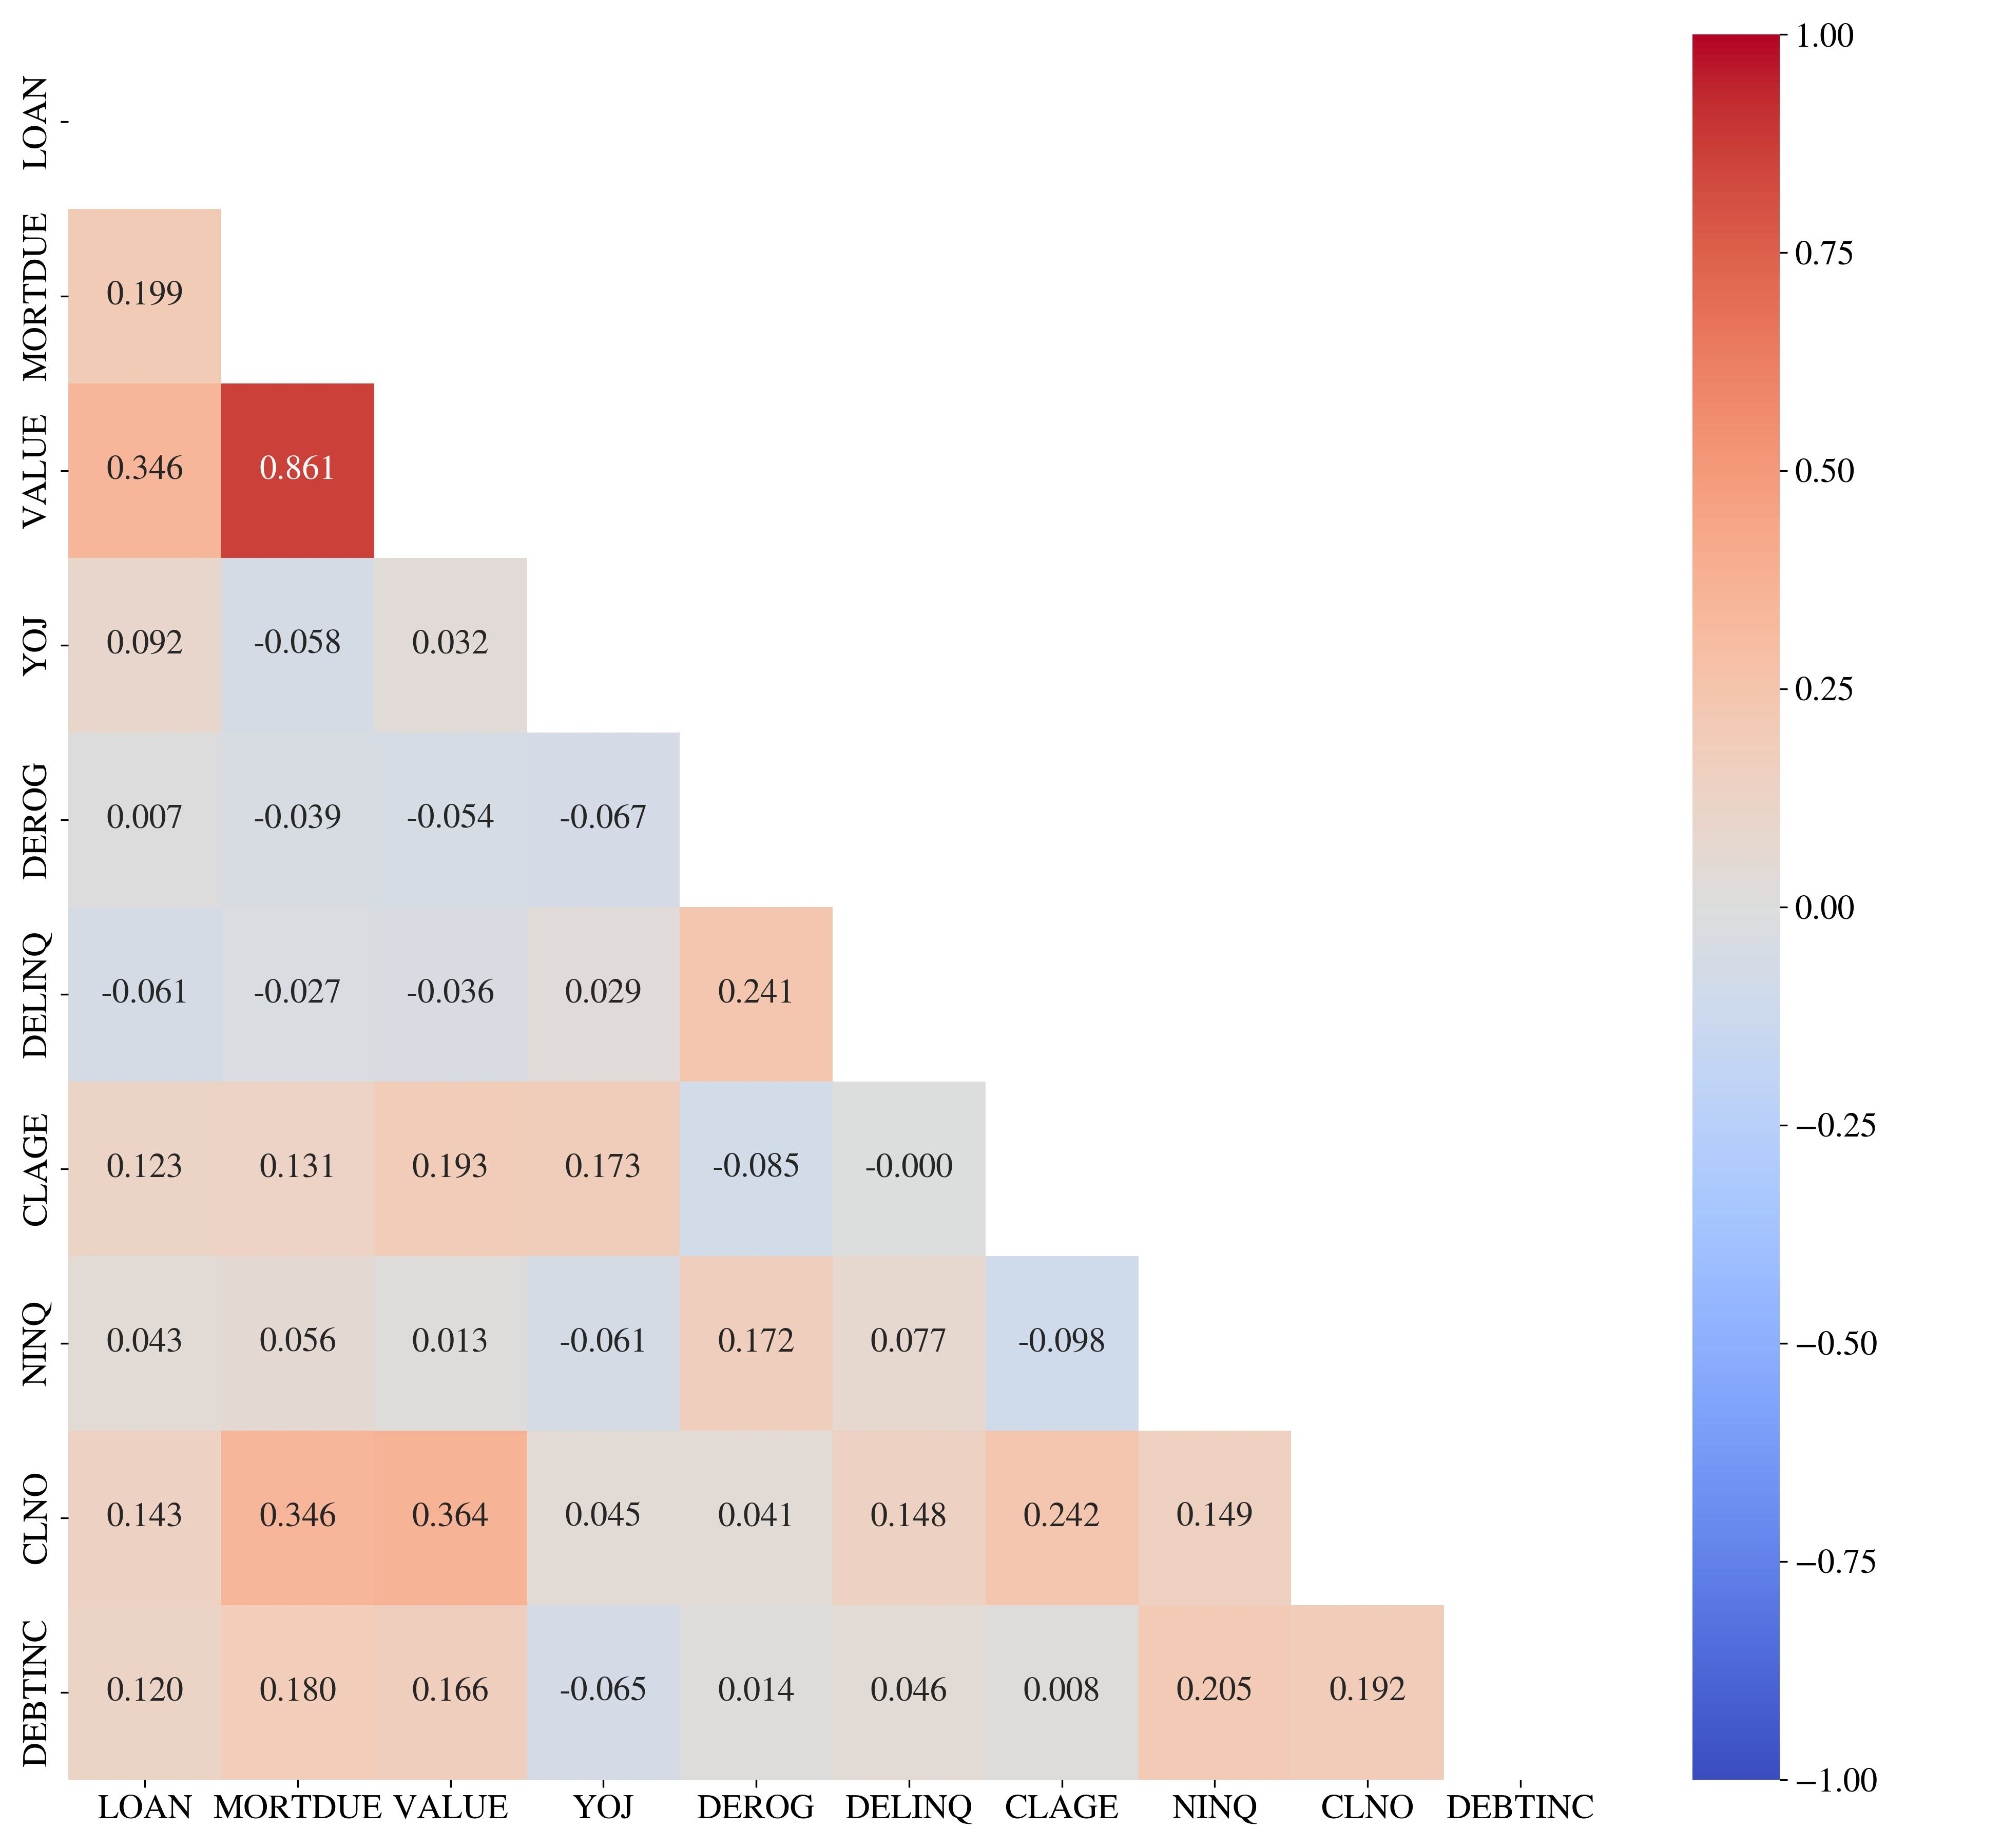
\includegraphics[width=150mm]{Figures/Spearman_Correlation_Matrix_Numeric_Features.jpg}
    \centering{\begin{source}Author's results in Python\end{source}}\vspace{-1em}
\end{figure}

\newpage
\section{Data Preprocessing}
In this section, the process of preprocessing data is described as the crucial step in the machine learning modelling. Particularly, the the process of dividing data for various tasks, oversampling due to the imbalanced class issue, discretization of features and Weight--of--Eveidence transformation are further discussed and described.

\subsection{Data Split and ADASYN Oversampling}
\label{subsec:data-split-ADASYN}

To ensure appropriate model training and unbiased evaluation, it is necessary to split data into separate sets for various purposes. Specifically, the data set is split into three sets: (1) training set for training the model, perform feature selection or hyperparameter tuning, (2) validation for hyperparameter tuning, and (3) test set for assess the model performance on the unseen data \citep{subasi2020practical}.
In this thesis, the data is plit into training, validation and test sets in ratio of 70:15:15, which ensures sufficient amount of data for training, hence the model would be able to generalize well, while keeping the validation and test sets large enough to provide reliable evaluation of the model's performance.

The data is split using stratified split to preserve the default status distribution, which is highly imbalanced.
Stratification ensures that the distribution of defaults and non-defaults remains the same across all sets, thereby avoiding overfitting and data leakage. Using stratification, each set had 80 \% non-defaults and 20 \% defaults. This method enables accurate prediction since the model is trained and evaluated on the same population \citep{igareta2021strat}.
However, stratification alone may not be sufficient for dealing with imbalanced classes. Therefore, ADASYN oversampling is performed as described in \autoref{sec:adasyntheory}. Note that ADASYN oversampling is performed on the training set only after the split to avoid data leakage and biased evaluation.

In Python, the data are divided and oversampled using a custom function \lstinline{data_split()}.
This function first employs the \lstinline{train_test_split()} function from the \lstinline{scikit-learn} module to split the data into training, validation, and test sets with a stratification technique.
Next, the \lstinline{ADASYN()} class from the \lstinline{imblearn} module is used to oversample the training set. This is achieved by generating synthetic instances of the minority class based on the five nearest neighbors and Euclidean distance.

However, the \lstinline{ADASYN()} class from \lstinline{imblearn} is not designed to handle missing values or categorical features encoded as character. To overcome this limitation, the following approach is taken:
\begin{enumerate}\setlength\itemsep{0em} 
\item Separate the categorical and numeric features;
\item Impute the missing values with arbitrary values:
\begin{itemize}
\item Categorical features: string \lstinline{'N/A'};
\item Numeric features: number \lstinline{99999999999999} - such value is chosen since it is highly unlikely to be present in the data set.
\end{itemize}
\item Convert the categorical features into dummy variables;
\item Join the numeric features with the dummy variables;
\item Perform the oversampling on the joined data set;
\item Convert the dummy variables back into categorical features;
\item Retrieve back the missing values:
\begin{itemize}
\item Categorical features: replace string \lstinline{'N/A'} with \lstinline{np.nan};
\item Numeric features: for each feature $X$ if its value exceeds the original maximum value, then replace it with \lstinline{np.nan};
\end{itemize}
\end{enumerate}


The following \autoref{tab:split} shows the default distribution of the individual sets before and after oversampling. The training set after ADASYN oversampling was balanced, while the default distribution remained the same across the validation and test sets before and after oversampling, which is desirable due to stratification.
\begin{table}[H]
\small
\setlength{\tabcolsep}{8pt}
\renewcommand{\arraystretch}{1.3}
\centering
    \caption[Sample sizes of split sets]{Sample sizes of split sets}\label{tab:split}
    \begin{tabular}{lrrr}
\toprule
\textbf{Set} & \textbf{\# instances} & \textbf{\% defaults} & \textbf{\% non--defaults}\\
\midrule
\hline
Training & 4,171  & 19.95 \% & 80.05 \% \\
Training (oversampled) & 6,437 &  48.13 \% & 51.87 \% \\

Validation & 895 &  20.00 \% & 80.00 \% \\

Test & 894 &  20.00 \% & 80.00 \% \\
\hline
\bottomrule
\end{tabular}
\vspace{0.7em}

\centering{\begin{source}Author's results in Python\end{source}}\vspace{-1em}
\end{table}

Since ADASYN increases the sample size by generating, i.e., adding new instances into the sample, it may have an impact on the distribution of the features.
After the inspection in Python, it have no significant impact on the numeric features as the distributions before and after ADASYN oversampling do not differ that much.
However, pertaining to the categorical features, a significant impact of ADASYN oversampling can be observed as can be seen in  \autoref{tab:adasynimpact} and \autoref{fig:adasynimpact}, respectively, which depict the distribution of categorical features on the subsample of default cases within the training set, particularly distribution before and after the oversampling.
As such, $n_B$ and $n_A$ refer to the number of default cases within given category before and after oversampling, respectively, $N_B$ and $N_A$ represents the total number of default cases before and after oversampling, respectively.

Within the \texttt{REASON} feature, we can observe a significant increase the proportion of defaulted clients who applied for a loan due to the debt consolidation (\texttt{DebtCon}) among all the defaulters after an oversampling - particularly, the ratio has increased by 12.20 percentage points.
On the other hand, the proportion of defaulted clients who applied for a loan due to the home improvement (\texttt{HomeImp}) has decreased by 9.69 percentage points, indicating lower distribution of such clients in the oversampled set.
Regarding the \texttt{JOB} feature, we can observe a substantial increase in the proportion in the of defaulted managers (\texttt{Mgr}) among all the defaulters after oversampling by 38.75 percentage points.
On the other hand, the proportion of defaulted clients who are labelled as \texttt{Others} has decreased by 17.15 percentage points.

\begin{table}[H]
    \small
    \setlength{\tabcolsep}{8pt}
    \renewcommand{\arraystretch}{1.3}
    \centering
    \caption[ADASYN Impact on Categorical Features' Distribution]{ADASYN Impact on Categorical Features' Distribution}\label{tab:adasynimpact}
    \begin{tabular}{|ll|rr|rr|r|}
    
        \hline
    Featuew & Category & $n_{B}$ & $n_{A}$ & $n_{B} / N_{B}$ &$n_{A} / N_{A}$ & Diff. \\ 
    \midrule
    \midrule
    REASON & DebtCon & 528 & 2,344 & 63.46 \% & 75.66 \% & 12.20 p.p. \\ 
    REASON & HomeImp & 274 & 720 & 32.93 \% & 23.24 \% & -9.69 p.p. \\
    REASON & N/A & 30 & 34 & 3.61 \% & 1.10 \% & -2.51 p.p. \\
    \hline
    JOB & Mgr & 124 & 1,662 & 14.9 \% & 53.65 \% & 38.75 p.p. \\ 
    JOB & Other & 396 & 943 & 47.6 \% & 30.44 \% & -17.16 p.p. \\ 
    JOB & ProfExe & 142 & 272 & 17.07 \% & 8.78 \% & -8.29 p.p. \\ 
    JOB & Office & 85 & 104 & 10.22 \% & 3.36 \% & -6.86 p.p. \\ 
    JOB & Self & 39 & 58 & 4.69 \% & 1.87 \% & -2.82 p.p. \\
    JOB & Sales & 29 & 36 & 3.49 \% & 1.16 \% & -2.33 p.p. \\ 
    JOB & N/A & 17 & 23 & 2.04 \% & 0.74 \% & -1.30 p.p. \\ 
    \hline
    \bottomrule
    \end{tabular}
    \vspace{0.7em}
    
    \centering{\begin{source}Author's results in Python\end{source}}\vspace{-1em}
\end{table}

Such findings regarding the significant increases in the proportion of default cases regarding the \texttt{DebtCon} and \texttt{Mgr} categories are given to the nature of ADASYN oversampling.
As explained before, ADASYN generates more synthetic default class instances in the neighborhood of such default instances, which are hard--to--learn for ADASYN.
In other words, ADASYN creates more default instances for such default instances where the density of the non--default class is relatively high in given default instance's neighborhood.
Therefore, default instances which either are managers or applied for a loan due to the debt consolidation are difficult--to--learn for ADASYN, thus ADASYN replicates more instances with such characteristics, hence this results in a higher proportion of default cases in the oversampled set for such category.


\begin{figure}[H]
    \centering
    \caption{ADASYN Impact of Categorical Features' Distribution}\vspace{0.5em}
    \label{fig:adasynimpact}\
    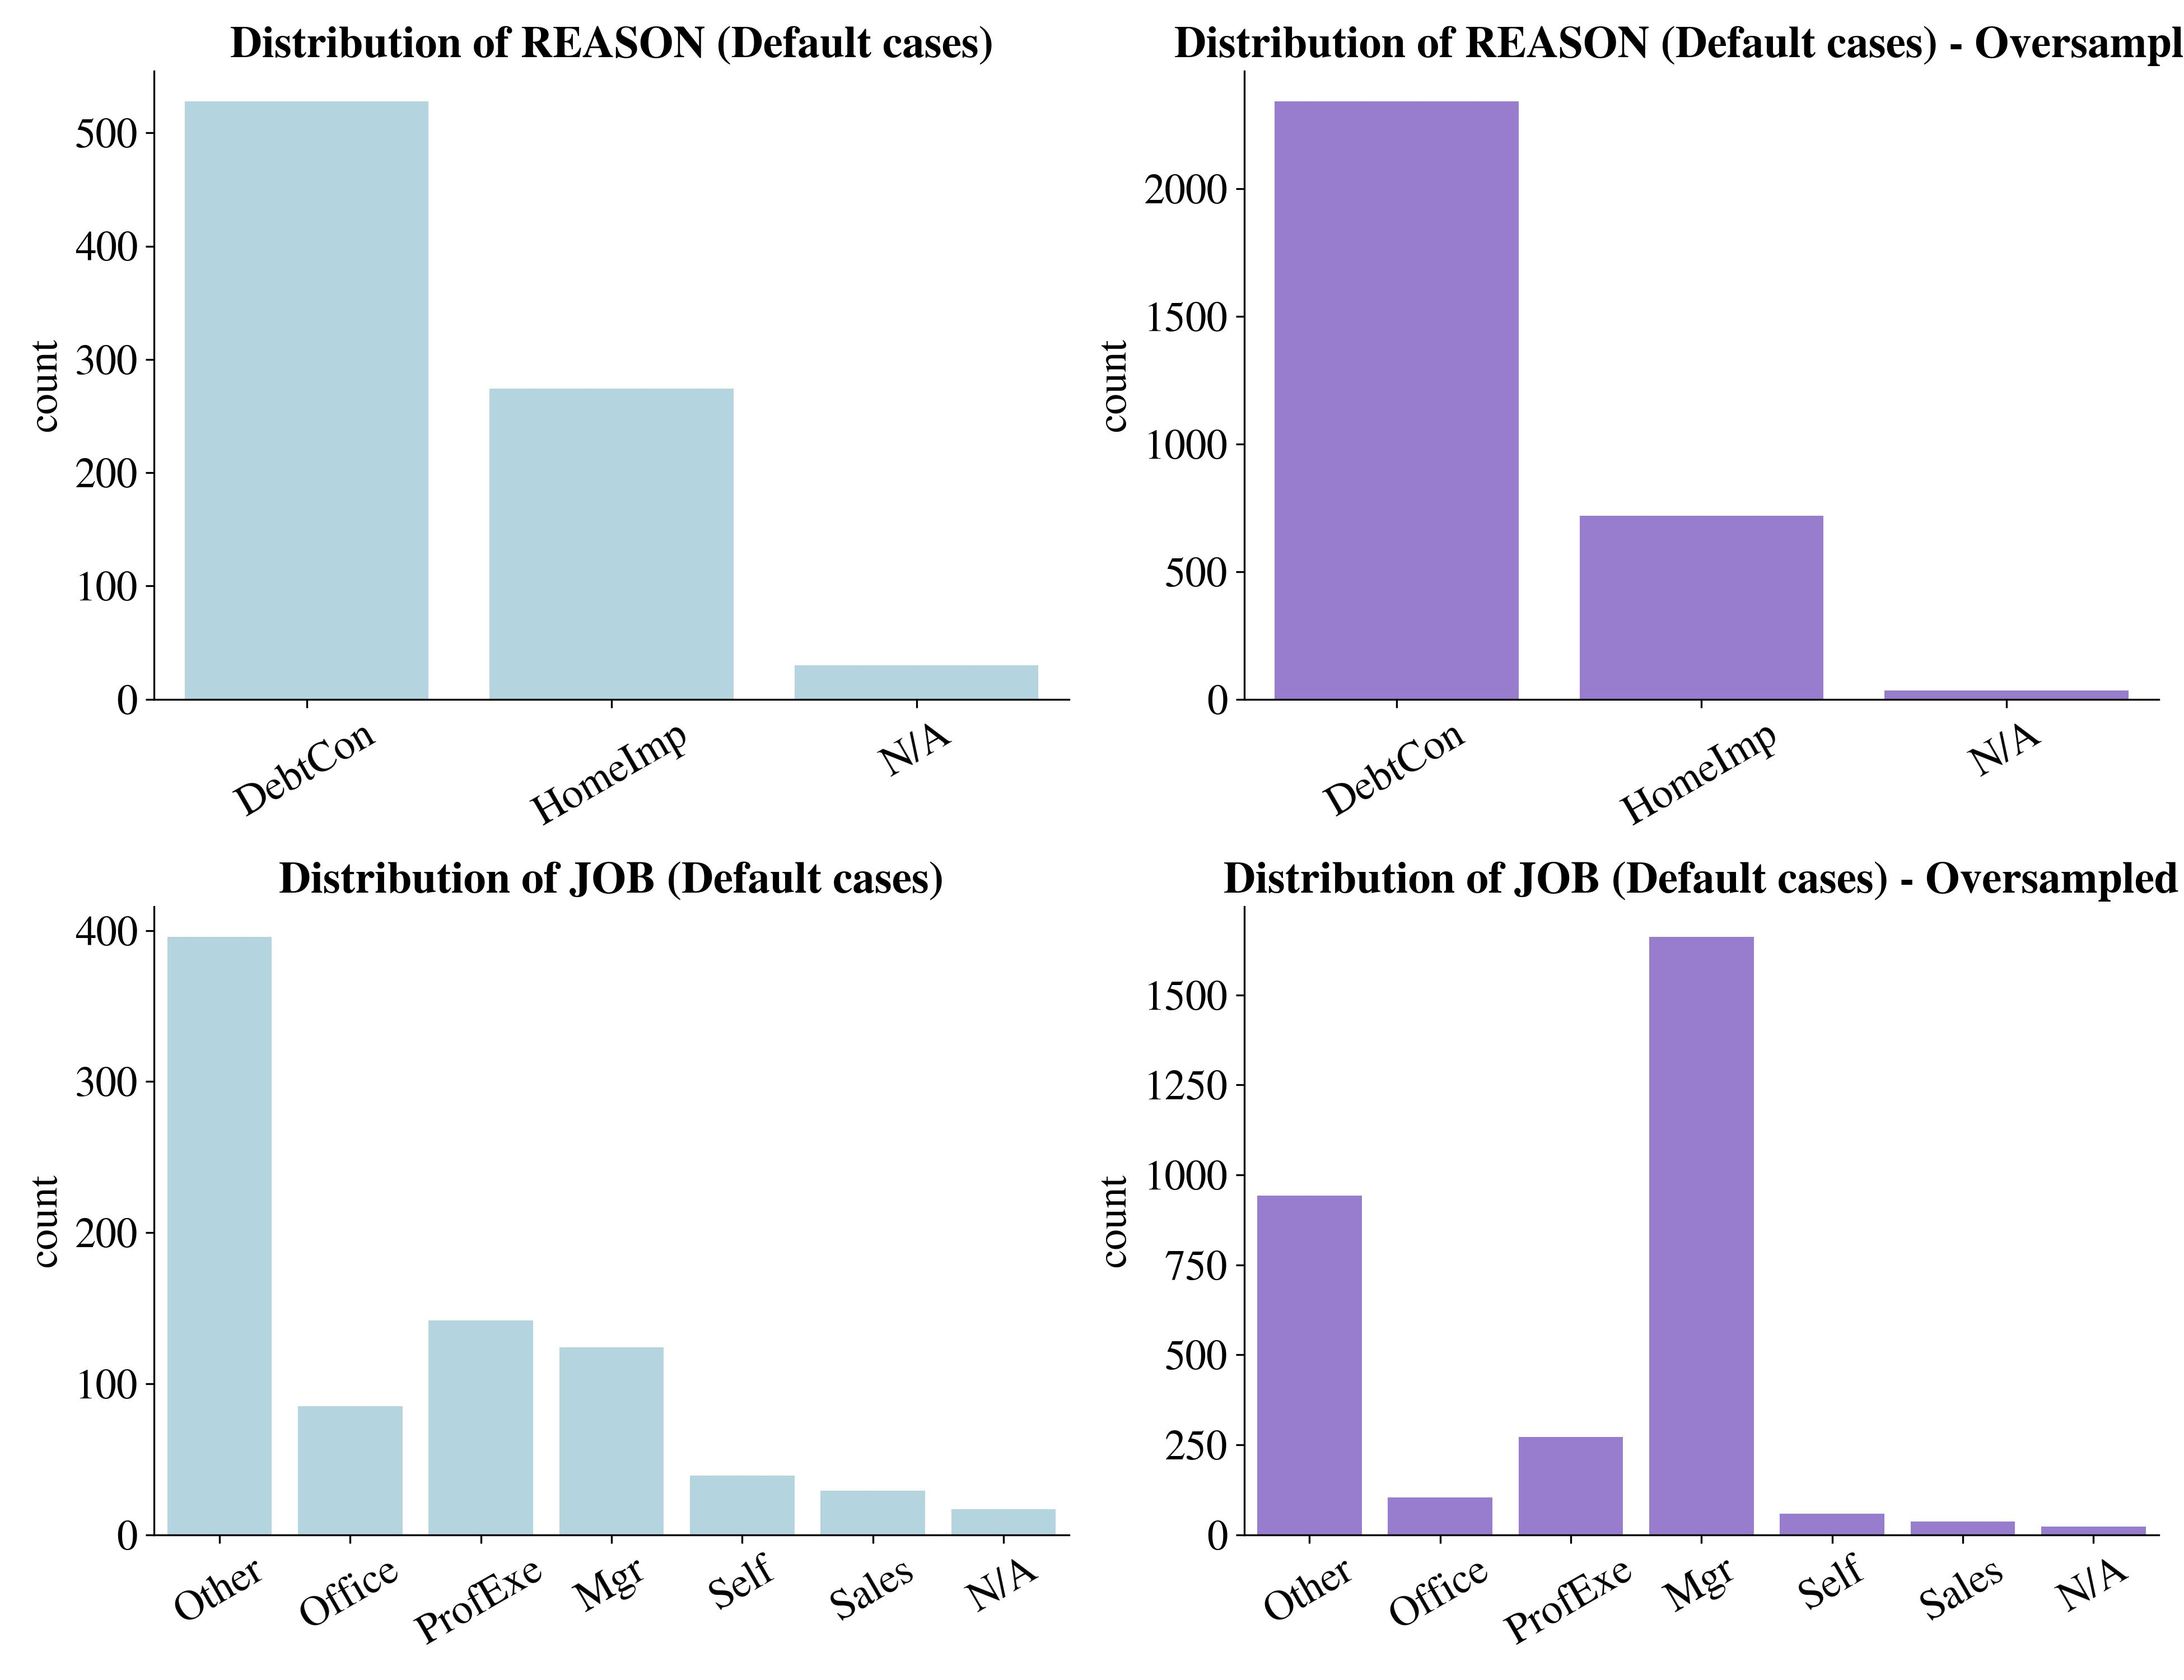
\includegraphics[width=140mm]{Figures/Categorical_Features_Distribution_OS_Default.jpg}
    \centering{\begin{source}Author's results in Python\end{source}}\vspace{-1em}
\end{figure}



\newpage
\subsection{Optimal Binning and Weight--of--Evidence}
\label{subsec:prep-optbinning}
As already described in autoref{sec:optbinningtheory}, the optimal binning is employed as a data preprocessing step in this thesis.
Particularly, we employ \lstinline{BinningProcess} class from the \lstinline{optbinning} module in Python - such class optimally discretizes the continuous features into interval bins and optimally groups categorical features' categories into sub-group categories with respect to the target variable while maximizing Information Value, and afterwards such bins are encoded using WoE \citep{navas2020optimal}. Besides discretizing and grouping, it also creates special bins for capturing missing values.


In this thesis, this data preprocessing step is wrapped into a custom function \lstinline{woe_binning()} in Python.
First, the  \lstinline{BinningProcess} class is fitted on the training set only in order to avoid data leakage, while it learns the split points for binning, event rates, WoE coefficients etc, and afterwards, such fitted  \lstinline{BinningProcess} class is used to transform training, validation and test set.


The following \autoref{fig:woedist} depicts the distribution of WoE bins for each feature. It can be observed that binning captures either linear, non-linear, monotonic, or non-monotonic relationships between the default status and the numeric features in terms of WoE.
Regarding the \texttt{DELINQ} feature, a monotonic relationship can be observed, where the higher number of delinquent credit lines, the lower the WoE coefficient, indicating a larger distribution of defaults with respect to non-defaults in the given bin.
Thus, the higher the number of delinquent credit lines, the higher the likelihood of defaulting in terms of WoE.

A non-linear relationship can be observed with respect to the \texttt{YOJ} feature, where the WoE coefficient is positive for applicants who have recently started working at their new job (i.e., number of years at the present job is less than 1) and for applicants who have been working at their current job for a relatively long time (i.e., number of years at the present job is higher than 19).
Thus, applicants who have been working for a longer time have stable income and are more creditworthy and less likely to default.
Regarding applicants who have recently started working at their new job, it is possible that they are less likely to default since the \texttt{YOJ} feature does not capture the applicant's total number of years of work experience, but only the number of years at the present job.
Thus, in the given data set, applicants who have recently started working at their new job have a relatively higher total number of years of work experience, making them more creditworthy and less likely to default. On the other hand, for applicants who have been working at their present job between 1 and 19 years, the WoE coefficient is negative.
This relationship seems to be complex and can be influenced by other factors not present in the data set, such as the applicant's age, total number of years of work experience, education, etc.

As already mentioned numeric and categorical features contain a separate bin capturing missing values, which can be a useful indicator when training a model. This is evident in the \texttt{DEBTINC} feature, where the bin capturing missing values has the most negative WoE coefficient, indicating that there is a larger distribution of defaulters compared to non-defaulters.
This finding was already raised in \autoref{subsubsec:target-na-ass} in terms of the strong and statistically significant association between the default status and the missing values in \texttt{DEBTINC}.

Within the \texttt{JOB} feature, specifically regarding the \texttt{Mgr} category, we can observe the direct impact of ADASYN oversampling as already described by \autoref{tab:adasynimpact}.
Since ADASYN generated more default class instances for original default instances who are managers, this results in higher default rate within such job category, thus to the larger distribution of defaulters compared to non--defaulters, which is quantified in the negative WoE value.

\textbf{QUESTION FOR SUPERVISOR: should I also decsribe the WoE distribution for other features as well or is this sufficient?}


\begin{figure}[H]
\centering
\caption{WoE Bins Distribution}\vspace{0.5em}
\label{fig:woedist}
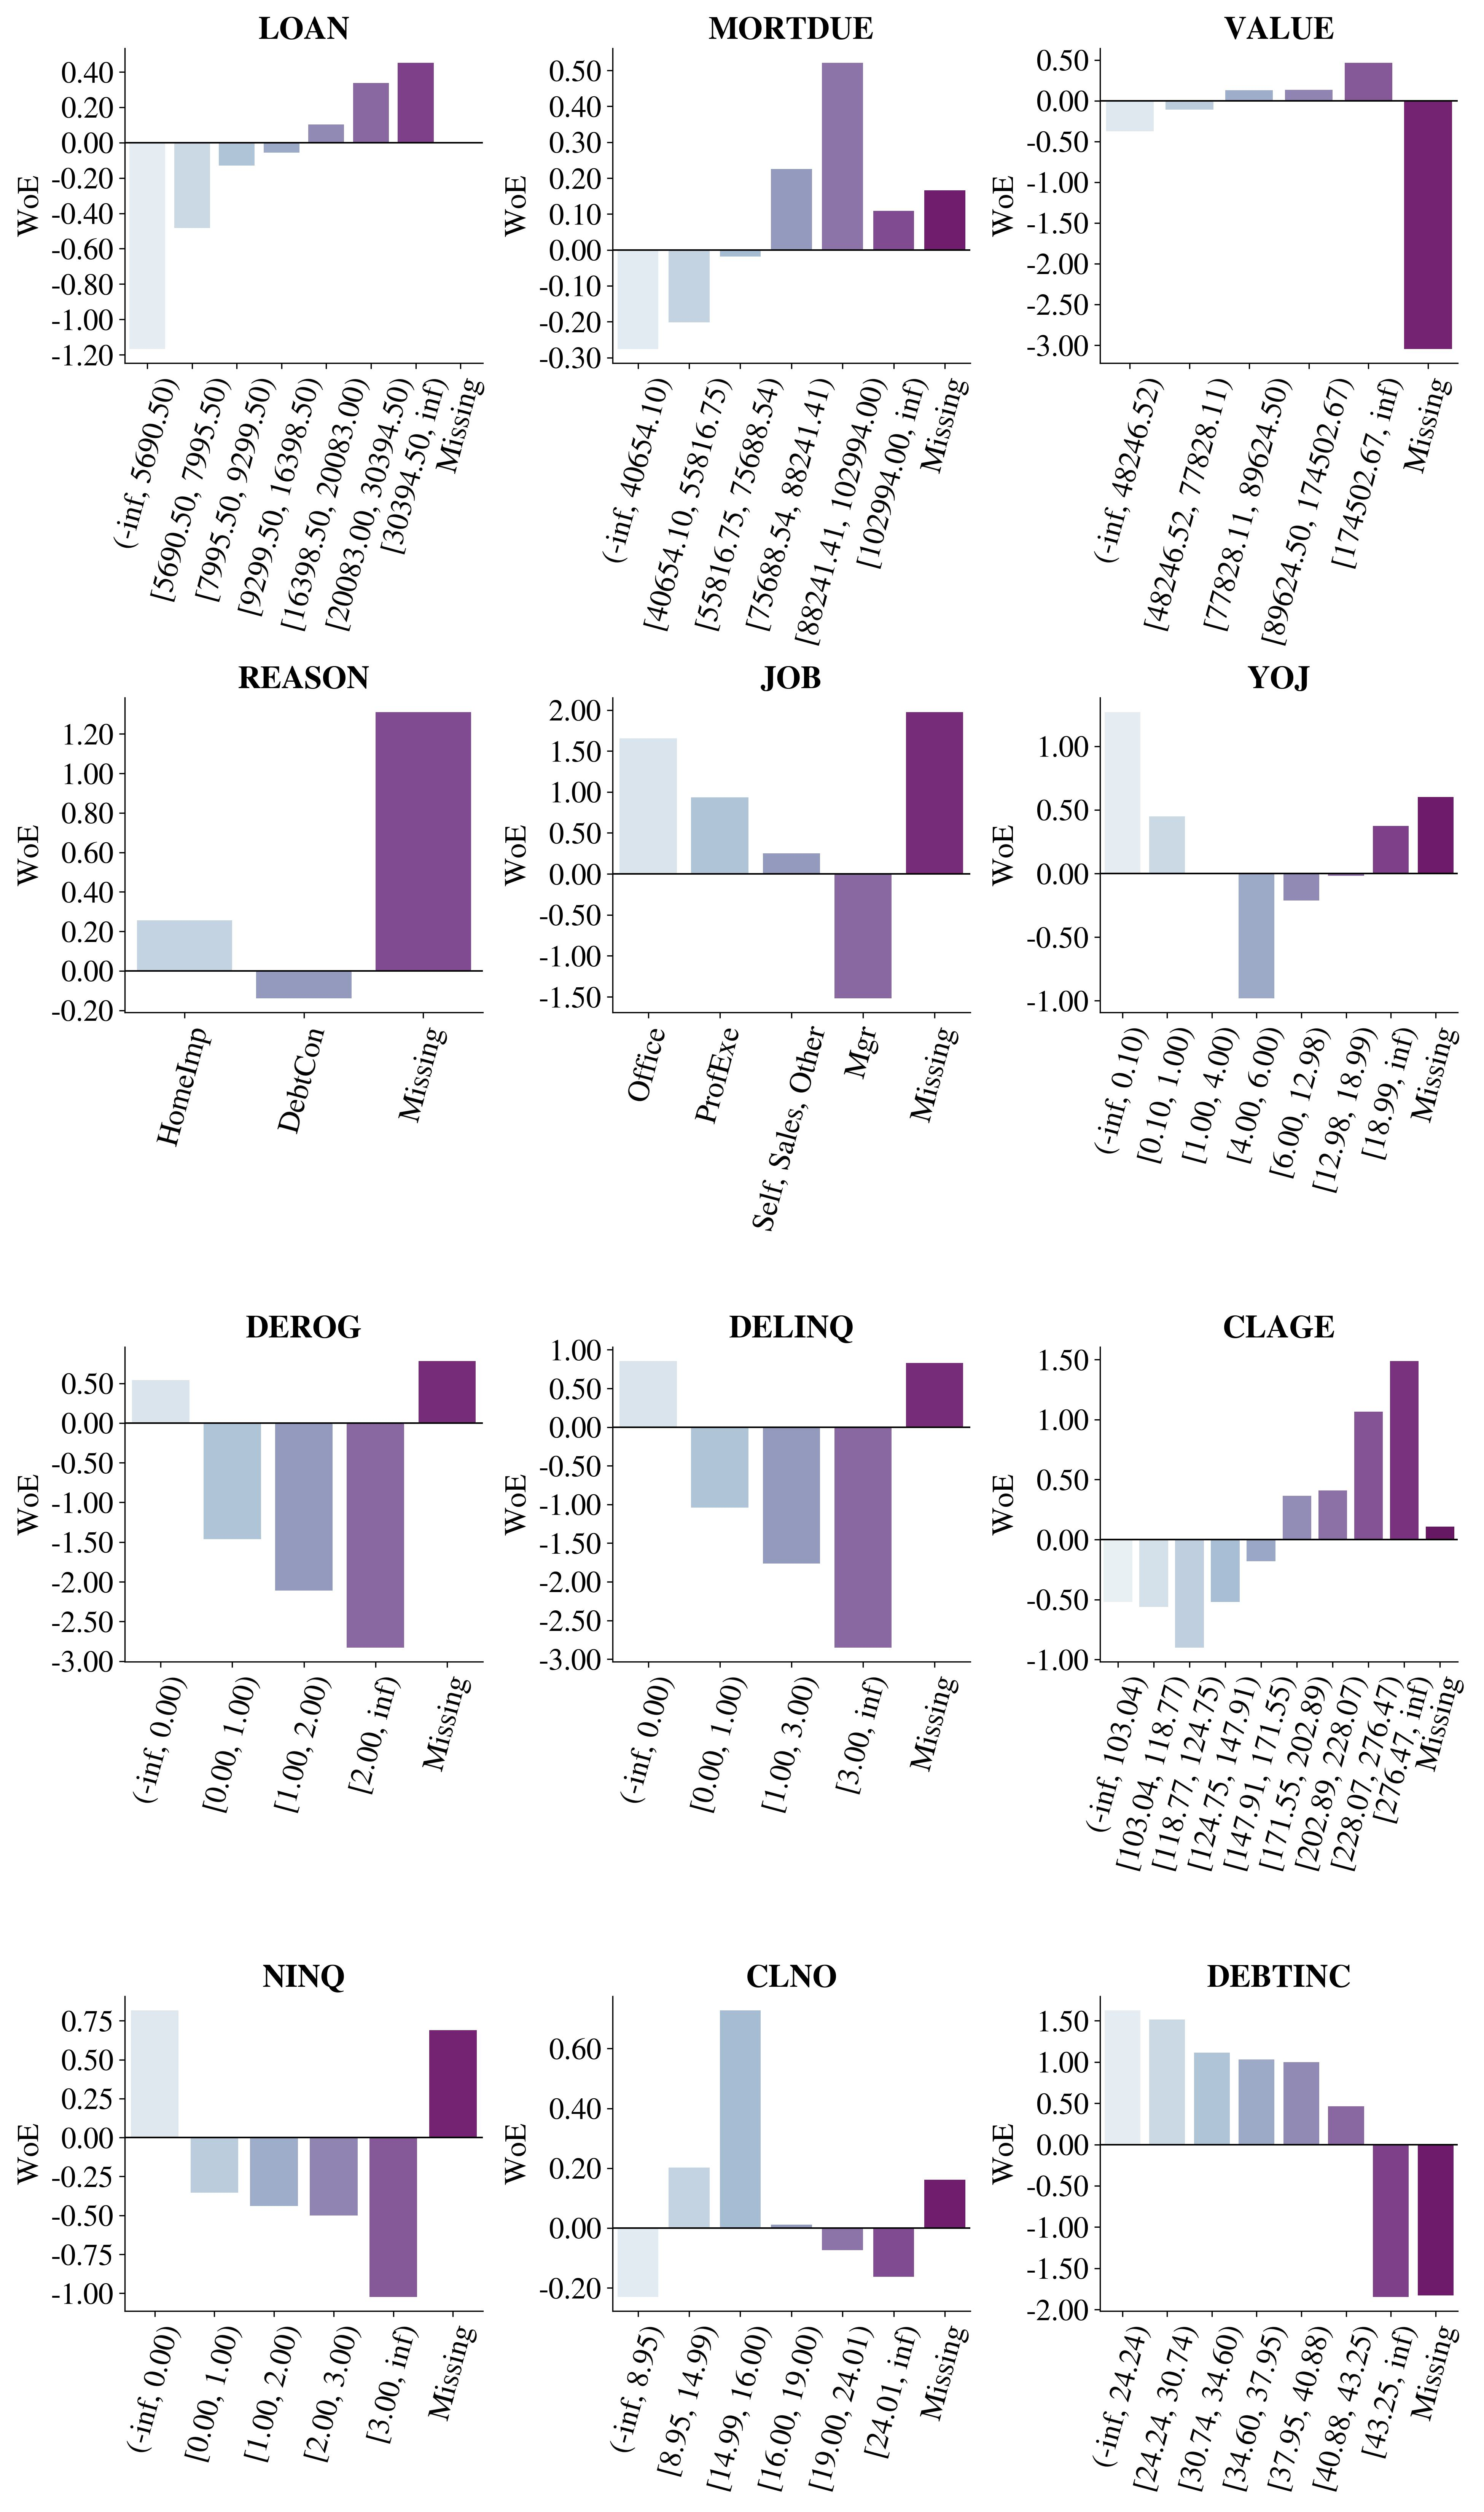
\includegraphics[width=140mm]{Figures/WoE_Distribution.jpg}
\centering{\begin{source}Author's results in Python\end{source}}\vspace{-1em}
\end{figure}

\newpage
\section{Modelling}
Once the data are finally preprocessed, the next step regards the modelling part which includes hyperparameter tuning, feature selection, model selection and model building.

In Python, 8 different machine learning models from \lstinline{Scikit-learn} module are used for the default status prediction, which were already described in \autoref{sec:algorithms}, namely:
\begin{itemize}\setlength\itemsep{0em}
\item \textbf{Logistic Regression} - \lstinline{LogisticRegression()}
\item \textbf{Decision Tree} - \lstinline{DecisionTreeClassifier()}
\item \textbf{Gaussian Naive Bayes} - \lstinline{GaussianNB()}
\item \textbf{K-Nearest Neighbors} - \lstinline{KNeighborsClassifier()}
\item \textbf{Random Forest} - \lstinline{RandomForestClassifier()}
\item \textbf{Gradient Boosting} - \lstinline{GradientBoostingClassifier()}
\item \textbf{Support Vector Machine} - \lstinline{SVC()}
\item \textbf{Multi--Layer Percepton} (\textit{Neural Network}) - \lstinline{MLPClassifier()}
\end{itemize}

\subsection{Hyperparameter Bayesian Optimization}
In this thesis, hyperparameter tuning of models is performed using Bayesian Optimization as described in \autoref{sec:bayesoptheory}.
In Python, a custom function, \lstinline{bayesian_optimization()}, is implemented to perform hyperparameter tuning using Bayesian Optimization.
This function utilizes \lstinline{BayesSearchCV} class from the \lstinline{Scikit-optimize} module, with a 10-fold stratified cross-validation scheme and 50 iterations, while maximizing the F1 score. As a surrogate function, Gaussian Process is used \citep{scikit-opt}.
The use of \lstinline{BayesSearchCV} with stratified cross-validation in the hyperparameter tuning process provides a robust and reliable approach to selecting the optimal hyperparameters for the model, while the incorporation of Bayesian Optimization enables the efficient exploration of the hyperparameter space.
By maximizing the F1 score, the hyperparameters selected through this process will result in a model with improved performance. Note, that the hyperparameter tuning is performed solely on training set in order to preserve the independence of the validation and test set, and avoid the information/data leakage as well.

For each model, the Bayesian Optimization algorithm performs 50 iterations while searching for the best hyperparameters values that maximize the F1 score. Within each iteration, a 10-fold stratified cross-validation is conducted to evaluate the model's cross--validation F1 score.
Moreover, for each model, we specify the hyperparameter space, i.e., particular hyperparameters to be tuned and their possible ranges which the hyperparameter can take. The ranges are specified using \lstinline{Integer} class to define interval of integers, \lstinline{Real} to define interval of float numbers, and \lstinline{Categorical} to define a list of possible (categorical) values.
Note that not all the available hyperparameters are tuned, but only the most relevants due to the time complexity of the Bayesian Optimization algorithm.
The definition of hyperparameter space for each model is described further in the following subsubsections.

\subsubsection{Logistic Regression}
The first hyperparameter \textbf{\texttt{Intercept}} allows to specify whether the intercept should be estimated or not.
The next hyperparameter is the \textbf{\texttt{C penalty factor}} as a regularization term to prevent overfitting by adding such term to the objective loss function \citep{pramoditha2021mitigate}. Particularly, in case of Logistic Regression, $C$ penalty factor is the regularization term which penalizes the coefficients' magnitudes.
The is related to the \textbf{\texttt{Penalty}} hyperparameter, which allows to specify the norm used in the penalization.
The most common penalty is $L1$ (also known as Lasso) penalty which which takes the absolute value of the coefficients' magnitudes.
The logistic regression's loss function is the cross--entropy (also known as Log Loss) which is further described in \autoref{subsubsec:logloss}. Then, the loss function with  $L1$ penalty is defined as follows:
\begin{equation}\label{eq}
    L(y, p)_{L1}  = L(y, p) + C \sum_{j=1}^{k} \mid w_j \mid
\end{equation}
Another penalty is $L2$ (also known as Ridge) penalty, which is more strict in penalization than $L1$ as it squares the coefficients' magnitudes. The loss function with $L2$ penalty is defined as follows:
\begin{equation}\label{eq}
    L(y, p)_{L2}  = L(y, p) + C \sum_{j=1}^{k} w_j^2
\end{equation}
The third penalty norm is the $ElasticNet$ which combines both $L1$ and $L2$. The loss function with $ElasticNet$ penalty is defined as follows:
\begin{equation}\label{eq}
    L(y, p)_{ElasticNet} = L(y, p) + C \sum_{j=1}^{k} \left[ \alpha \mid w_j \mid + (1-\alpha) w_j^2 \right]
\end{equation}
where $\alpha$ indicates the weight of $L1$ penalty in the $ElasticNet$ penalty and refers to the \textit{L1 ratio} hyperparameter.
Moreover, the  \textbf{\texttt{Class weight}} hyperparameter is a hyperparameter which allows to assign higher importance to the minority class instances during the training process.


Furthermore, \textbf{\texttt{Solver}} hyperparameter is used to specify which optimization algorithm should be used to estimate the coefficients' values.
According to Hale \citep{hale2019dont}, Scikit-learn provides five solvers for Logistic Regression, namely \textit{lbfgs} (Limited-memory Broyden-Fletcher-Goldfarb-Shanno) which approximates the second derivative matrix updates with gradient evaluations, \textit{liblinear} (Library for Large Linear Classification) which uses coordinate descent algorithm, \textit{newton-cg},
\textit{sag} (Stochastic Average Gradient descent) as a variation of gradient descent and incremental aggregated gradient approaches using random sample of previous gradient values, and \textit{saga} as an extension of \textit{sag} which allows $L1$ regularization.
For more information, please refer to the Scikit-learn documentation regarding Logistic Regression \citep{scikit-lr}.
The last hyperparameter of Logistic Regression to tune in this thesis is the \textbf{\texttt{Intercept scaling}} which allows to scale the intercept.

\begin{table}[H]
\small
\setlength{\tabcolsep}{8pt}
\renewcommand{\arraystretch}{1.3}
\centering
    \caption[Logistic Regression - Hyperparameter Space]{Logistic Regression - Hyperparameter Space}\label{tab:lrspace}
    \begin{tabular}{ll}
\toprule
\textbf{Hyperparameter} & \textbf{Space}\\
\midrule
\hline
Intercept & True, False \\
$C$ factor & <$1\times10^{-6}$, 5>\\
Penalty & L1, L2, Elastic Net, None \\
Solver & lbfgs, liblinear, newton-cg, sag, saga \\
Class weight & None, balanced \\
L1 ratio & <0, 1> \\
Intercept scaling & True, False  \\
\hline
\bottomrule
\end{tabular}
\vspace{0.7em}

\centering{\begin{source}Author's results in Python\end{source}}\vspace{-1em}
\end{table}


\subsubsection{Decision Tree}
The first hyperparameter of Decision Tree is the \textbf{\texttt{Criterion}} which allows to specify the function to measure the quality of a split - either Gini or Entropy impurity function.
Another important hyperparameter is the \textbf{\texttt{Max depth}} which allows to specify the maximum depth of the tree.
The last hyperparameter is the \textbf{\texttt{Max features}} which allows to specify the number of features to consider when looking for the best split \citep{scikit-dt}.
Note, that \textbf{\texttt{Max features}} has a variable range of values depending on the number of features which is dependent on the number of features selected during feature selection (where the feature are iteratively selected and the model is trained and evaluated on each iteration).
\begin{table}[H]
\small
\setlength{\tabcolsep}{8pt}
\renewcommand{\arraystretch}{1.3}
\centering
    \caption[Decision Tree - Hyperparameter Space]{Decision Tree - Hyperparameter Space}\label{tab:dtspace}
    \begin{tabular}{ll}
\toprule
\textbf{Hyperparameter} & \textbf{Space}\\
\midrule
\hline
Criterion & Gini, Entropy \\
Max depth & <1, 10> \\
Max features & <1, \verb|len(X.columns)|>  \\
\hline
\bottomrule
\end{tabular}
\vspace{0.7em}

\centering{\begin{source}Author's results in Python\end{source}}\vspace{-1em}
\end{table}

\subsubsection{Gaussian Naive Bayes}

In case of Gaussian Naive Bayes, the only hyperparameter to tune is the \textbf{\texttt{Variance smoothing}} which allows to specify the portion of the largest variance of all features to be added to variances for calculation stability \citep{scikit-gnb}, in order to smooth out the variances of each feature in case when the variance is zero.
\begin{table}[H]
\small
\setlength{\tabcolsep}{8pt}
\renewcommand{\arraystretch}{1.3}
\centering
    \caption[Gaussian Naive Bayes - Hyperparameter Space]{Gaussian Naive Bayes  - Hyperparameter Space}\label{tab:gnbspace}
    \begin{tabular}{ll}
\toprule
\textbf{Hyperparameter} & \textbf{Space}\\
\midrule
\hline
Variance smoothing & <$1\times 10^{-9}$, $1\times 10^{-6}$> \\
\hline
\bottomrule
\end{tabular}
\vspace{0.7em}

\centering{\begin{source}Author's results in Python\end{source}}\vspace{-1em}
\end{table}


\subsubsection{K--Nearest Neighbors}

In KNN, it is crucial to specify the number of neighbors to consider during the classification process, which is depicted in the \textbf{\texttt{\# neighbors}} hyperparameter.
Further, it is needed to select optimal distance measure, i.e., Euclidean, Manhattan or Minkowski as described in \autoref{subsec:knn-theory} - such selection refers to the \textbf{\texttt{Metric}} hyperparameter.
Pertaining to the Minowski distance, we tune also the \textbf{\texttt{Norm order}} hyperparameter which allows to specify the power parameter within the distance calculation.
Last but not least, KNN also allows to tune the \textbf{\texttt{Weights}} hyperparameter which allows to specify the weight function used in prediction - either uniform or distance. With the former function, all the points within each neighborhood are weighted uniformly and with the latter approach, the points are weighted inversely with respect to their distance. \citep{scikit-knn}.
\begin{table}[H]
\small
\setlength{\tabcolsep}{8pt}
\renewcommand{\arraystretch}{1.3}
\centering
    \caption[K--Nearest Neighbors - Hyperparameter Space]{K--Nearest Neighbors - Hyperparameter Space}\label{tab:knnspace}
    \begin{tabular}{ll}
\toprule
\textbf{Hyperparameter} & \textbf{Space}\\
\midrule
\hline
\# neighbors & <5, 20> \\
Metric & Euclidean, Manhattan, Minkowski \\
Norm order & <1, 5> \\
Weights & Uniform, Distance \\
\hline
\bottomrule
\end{tabular}
\vspace{0.7em}

\centering{\begin{source}Author's results in Python\end{source}}\vspace{-1em}
\end{table}

\subsubsection{Random Forest}
In in the Random Forest, we tune the number of base trees which are trained in parallel way in the ensemble, i.e., the \textbf{\texttt{\# estimators}} hyperparameter. 
Similarly to Decision Tree, Random Forest allows to select the optimal split measure, i.e., Gini, Entropy or additionaly even Log Loss, which is depicted in the \textbf{\texttt{Criterion}} hyperparameter.
Likewise Decision Tree, Random Forest also allows to specify the maximum depth of the tree as well as the  the number of features to consider when looking for the best split, i.e., the \textbf{\texttt{Max depth}} hyperparameter and \textbf{\texttt{Max features}}, respectively.
The \textbf{\texttt{Bootstrap}} hyperparameter allows to specify whether bootstrap samples are used when training the tree estimators.
Similarly to Logistic Regression, Random Forest also has the \textbf{\texttt{Class weight}} hyperparameter which allows to specify the weight of each class in the classification process - \textit{balanced} function takes the target variable to adjust the weights which are inversely proportional to class frequencies, whereas \textit{subsample balanced} does almost the same, but the weights are computed based on the bootstrap samples.
Last but not least, Random Forest also allows to tune the \textbf{\texttt{CCP alpha}} hyperparameter which allows to specify the complexity parameter used for Minimal Cost-Complexity Pruning (CCP), in order to reduce the size of the tree estimators and avoid overfitting by remocing subtrees from the tree estimators which do not improve the performance \citep{scikit-rf}.

\begin{table}[H]
\small
\setlength{\tabcolsep}{8pt}
\renewcommand{\arraystretch}{1.3}
\centering
    \caption[Random Forest - Hyperparameter Space]{Random Forest - Hyperparameter Space}\label{tab:rfspace}
    \begin{tabular}{ll}
\toprule
\textbf{Hyperparameter} & \textbf{Space}\\
\midrule
\hline
\# estimators & <100, 1000> \\
Criterion & Gini, Entropy, Log Loss \\
Max depth & <1, 10> \\
Max features & <1, \verb|len(X.columns)|>  \\
Bootstrap & True, False \\
Class weight & None, balanced, subsample balanced \\
CCP alpha & <$1\times10^{-12}$, 0.5> \\
\hline
\bottomrule
\end{tabular}
\vspace{0.7em}

\centering{\begin{source}Author's results in Python\end{source}}\vspace{-1em}
\end{table}

\subsubsection{Gradient Boosting}
Likewise Random Forest, Gradient Boosting also allows to tune the number of base trees which are trained in sequential way in the ensemble, i.e., the \textbf{\texttt{\# estimators}} hyperparameter, as well as the maximum depth of the tree and the number of features to consider when looking for the best split, i.e., the \textbf{\texttt{Max depth}} hyperparameter and \textbf{\texttt{Max features}}, respectively.
Is it also need to tune the \textbf{\texttt{Learning rate}} hyperparameter which shrinks the contribution of each tree in order prevent overfitting.
We can also select the optimal loss function of Gradient Boosting (\textbf{\texttt{Loss}} hyperparameter), either Log Log Loss or Exponential loss function - in the latter case, the model is equivalent to AdaBoost algorithm \citep{scikit-gb}.
Moreover, the \textbf{\texttt{Criterion}} hyperparameter allows to specify measurement method of the split quality, i.e., MSE or Friedman MSE which improves the MSE with Friedman scores \citep{scikit-gb}.

\begin{table}[H]
\small
\setlength{\tabcolsep}{8pt}
\renewcommand{\arraystretch}{1.3}
\centering
    \caption[Gradient Boosting - Hyperparameter Space]{Gradient Boosting - Hyperparameter Space}\label{tab:gbspace}
    \begin{tabular}{ll}
\toprule
\textbf{Hyperparameter} & \textbf{Space}\\
\midrule
\hline
\# estimators & <100, 1000> \\
Max depth & <1, 10> \\
Max features & <1, \verb|len(X.columns)|>  \\
Learning rate & <0.0001, 0.2> \\
Loss & Log Loss, Exponential \\
Criterion & MSE, Friedman MSE \\
\hline
\bottomrule
\end{tabular}
\vspace{0.7em}

\centering{\begin{source}Author's results in Python\end{source}}\vspace{-1em}
\end{table}

\subsubsection{Support Vector Machine}
Likewise Logistic Regression, SVM also allows to tune the \textbf{\texttt{C}} hyperparameter for the regularization, as well as the \textbf{\texttt{Kernel}} hyperparameter which specifies the kernel type to be used in the algorithm in order to map the data into higher dimensional space in order to find the optimal hyperplane which separates the classes.
If the kernel is $d$-degree polynomial, we can also tune the \textbf{\texttt{Degree}} hyperparameter which specifies the degree of the polynomial kernel function.
SVM also has the \textbf{\texttt{Class weight}} hyperparameter which assigns the weights to the input data based on the class frequencies in order to balance the classes.


\begin{table}[H]
\small
\setlength{\tabcolsep}{8pt}
\renewcommand{\arraystretch}{1.3}
\centering
    \caption[Support Vector Machine - Hyperparameter Space]{Support Vector Machine - Hyperparameter Space}\label{tab:svmspace}
    \begin{tabular}{ll}
\toprule
\textbf{Hyperparameter} & \textbf{Space}\\
\midrule
\hline
C factor & <$1\times 10^{-6}$, 5> \\
Kernel & Linear, Poly, RBF, Sigmoid \\
Degree & <1, 10> \\
Class weight & balanced, None \\
\hline
\bottomrule
\end{tabular}
\vspace{0.7em}

\centering{\begin{source}Author's results in Python\end{source}}\vspace{-1em}
\end{table}


\subsubsection{Multi--Layer Percepton}
\textbf{TBD}

In the MLP, we tune the activation function applied in the hidden layers, namely Logistic, ReLU, Tanh which were already described in \autoref{subssec:nn}, and further Identity which is just a linear activation function, hence $f(z) = z$.
Regarding the optimization algorithm which refers to \textbf{\texttt{Solver}} hyperparameter, we can choose between \textit{lbgfs}, \textit{sgd} (Stochastic Gradient Descent) and \textit{adam} (Adaptive Moment Estimation).
The \textbf{\texttt{Learning rate}} can be either constant (i.e, 0.001), inversely scaled, i.e., gradually and inversely decreased with and inverse scaling exponent $t$ (where $t$ refers to the time step, by default $t=0.5$), or adaptive, i.e., the learning rate is kept constant as long as the training loss keeps decreasing, otherwise it is divided by 5 \citep{scikit-mlp}.

\begin{table}[H]
\small
\setlength{\tabcolsep}{8pt}
\renewcommand{\arraystretch}{1.3}
\centering
    \caption[Multi Layer Percepton - Hyperparameter Space]{Multi Layer Percepton - Hyperparameter Space}\label{tab:mlpspace}
    \begin{tabular}{ll}
\toprule
\textbf{Hyperparameter} & \textbf{Space}\\
\midrule
\hline
Hidden layer size & <5, 500> \\
Activation function & Identity, Logistic, Tanh, ReLU \\
Solver & Adam, sgd, lbfgs \\
Learning rate & Constant, Adaptive, Invscaling \\
\hline
\bottomrule
\end{tabular}
\vspace{0.7em}

\centering{\begin{source}Author's results in Python\end{source}}\vspace{-1em}
\end{table}

\newpage
\subsection{Sequential Feature Selection}
\label{subsec:feature-selection}

As the feature selection approach, Forward Sequential Feature Selection is employed in order to choose the optimal set of features as described in \autoref{sec:fsfstheory}.
Within machine learning implemenation, instead of fitting Forward SFS only with one model, Forward SFS is fitted for each input model in order to obtain the best subsets of features for each model, assuming the importance of each features varies across the models.
Instead of using input models with default hyperparameters, each model is tuned with Bayesian Optimization in order to obtain the optimal hyperparameters for each model, which would further improve the performance of each model within SFS and therefore, it would lead to the more optimal selection of features.
The custom feature selection algorithm is stated in Algorithm \autoref{alg:feature_selection}, thus, when having $n$ input models, it returns $n$  subsets of optimal features, one per each model:
\begin{algorithm}[H]
\caption{Feature Selection Algorithm}
\label{alg:feature_selection}
\begin{algorithmic}[1]
\For{$model \in \textit{models}$}
    \State $\textit{optimized\_model} \gets \textsc{BayesianOptimization}(model)$
    \State $\textit{best\_features} \gets \textsc{ForwardSFS}(\textit{optimized\_model})$
\EndFor
\end{algorithmic}
\end{algorithm}
Particularly, each input model is first tuned on the training set with Bayesian Optimization with 50 iterations and 10--fold stratified cross validation (in order to preserve the target variable distribution across the folds) while maximizing the F1 score - within author's machine learning implemenation, his custom function \lstinline{bayesian_optimization()} is used.
Once the model is tuned, the Forward SFS is fitted with such tuned model on the same training set with 10--fold stratified cross validation while maximizing the F1 score. Instead of selecting the fixed number of features, Scikit-learn's \lstinline{SequentialFeatureSelector} class allows to set a stop criterion (\lstinline{tol} parameter) which stops adding features if the objective score function is not increasing at least by \lstinline{tol} between two consecutive feature additions \citep{sfs}.
Such paramaeter is set to the value which is close to zero, therefore the feature selection stops when the objective score function is not increasing anymore.

Such feature selection algorithm is wrapped into author's custom function \lstinline{SFS_feature_selection()}.
This function iteratively prints the process of the feature selection as can be seen in \autoref{fig:featselectprint}, including the current step (Bayesian Optimization or Feature Selection), the execution time in minutes, and the selected features per each model. Since we have 8 input models, we get 8 optimal subsets of features.

\begin{figure}[H]
\centering\caption{Feature Selection Print Statement}
\label{fig:featselectprint}

{\fontsize{8.8}{11}\selectfont 
\begin{verbatim}
-------------------------------------------------------------------------------------
------------------------------------------ 2/8 --------------------------------------
-------------------------------------------------------------------------------------
------------------------------- FEATURE SELECTION WITH DT ---------------------------
-------------------------------------------------------------------------------------
------------------------------------------------------------------------------------- 

1/4 ... Starting Bayesian Optimization on the whole set of features
2/4 ... Bayesian Optimization finished
3/4 ... Starting Forward Sequential Feature Selection
4/4 ... Forward Sequential Feature Selection with finished 

Execution time: 0.8622 minutes 

9 features selected: VALUE, JOB, YOJ, DEROG, DELINQ, CLAGE, NINQ, CLNO, DEBTINC 

-------------------------------------------------------------------------------------
------------------------------------------------------------------------------------- 


-------------------------------------------------------------------------------------
------------------------------------------ 3/8 --------------------------------------
-------------------------------------------------------------------------------------
------------------------------- FEATURE SELECTION WITH GNB --------------------------
-------------------------------------------------------------------------------------
------------------------------------------------------------------------------------- 

1/4 ... Starting Bayesian Optimization on the whole set of features
2/4 ... Bayesian Optimization finished
3/4 ... Starting Forward Sequential Feature Selection
4/4 ... Forward Sequential Feature Selection with finished 

Execution time: 0.4152 minutes 

6 features selected: MORTDUE, JOB, DELINQ, CLAGE, NINQ, DEBTINC 

------------------------------------------------------------------------------------- 
------------------------------------------------------------------------------------- 
\end{verbatim}
}
\centering{\begin{source}Author's results in Python\end{source}}\vspace{0em}
\end{figure}


The following \autoref{fig:fsrec} depicts the reccurrence of the selected features. As can be seen, features such as \texttt{CLAGE}, \texttt{DEBTINC}, \texttt{DELINQ} and \texttt{JOB} were selected by each model. 
On the other hand, features such as \texttt{LOAN} and \texttt{REASON} were selected only four times. Therefore, it can be expected that such features which were selected every time will have significant impact in predictions.
\begin{figure}[H]
\centering
\caption{Reccurrence of Selected Features}\vspace{0.5em}
\label{fig:fsrec}\
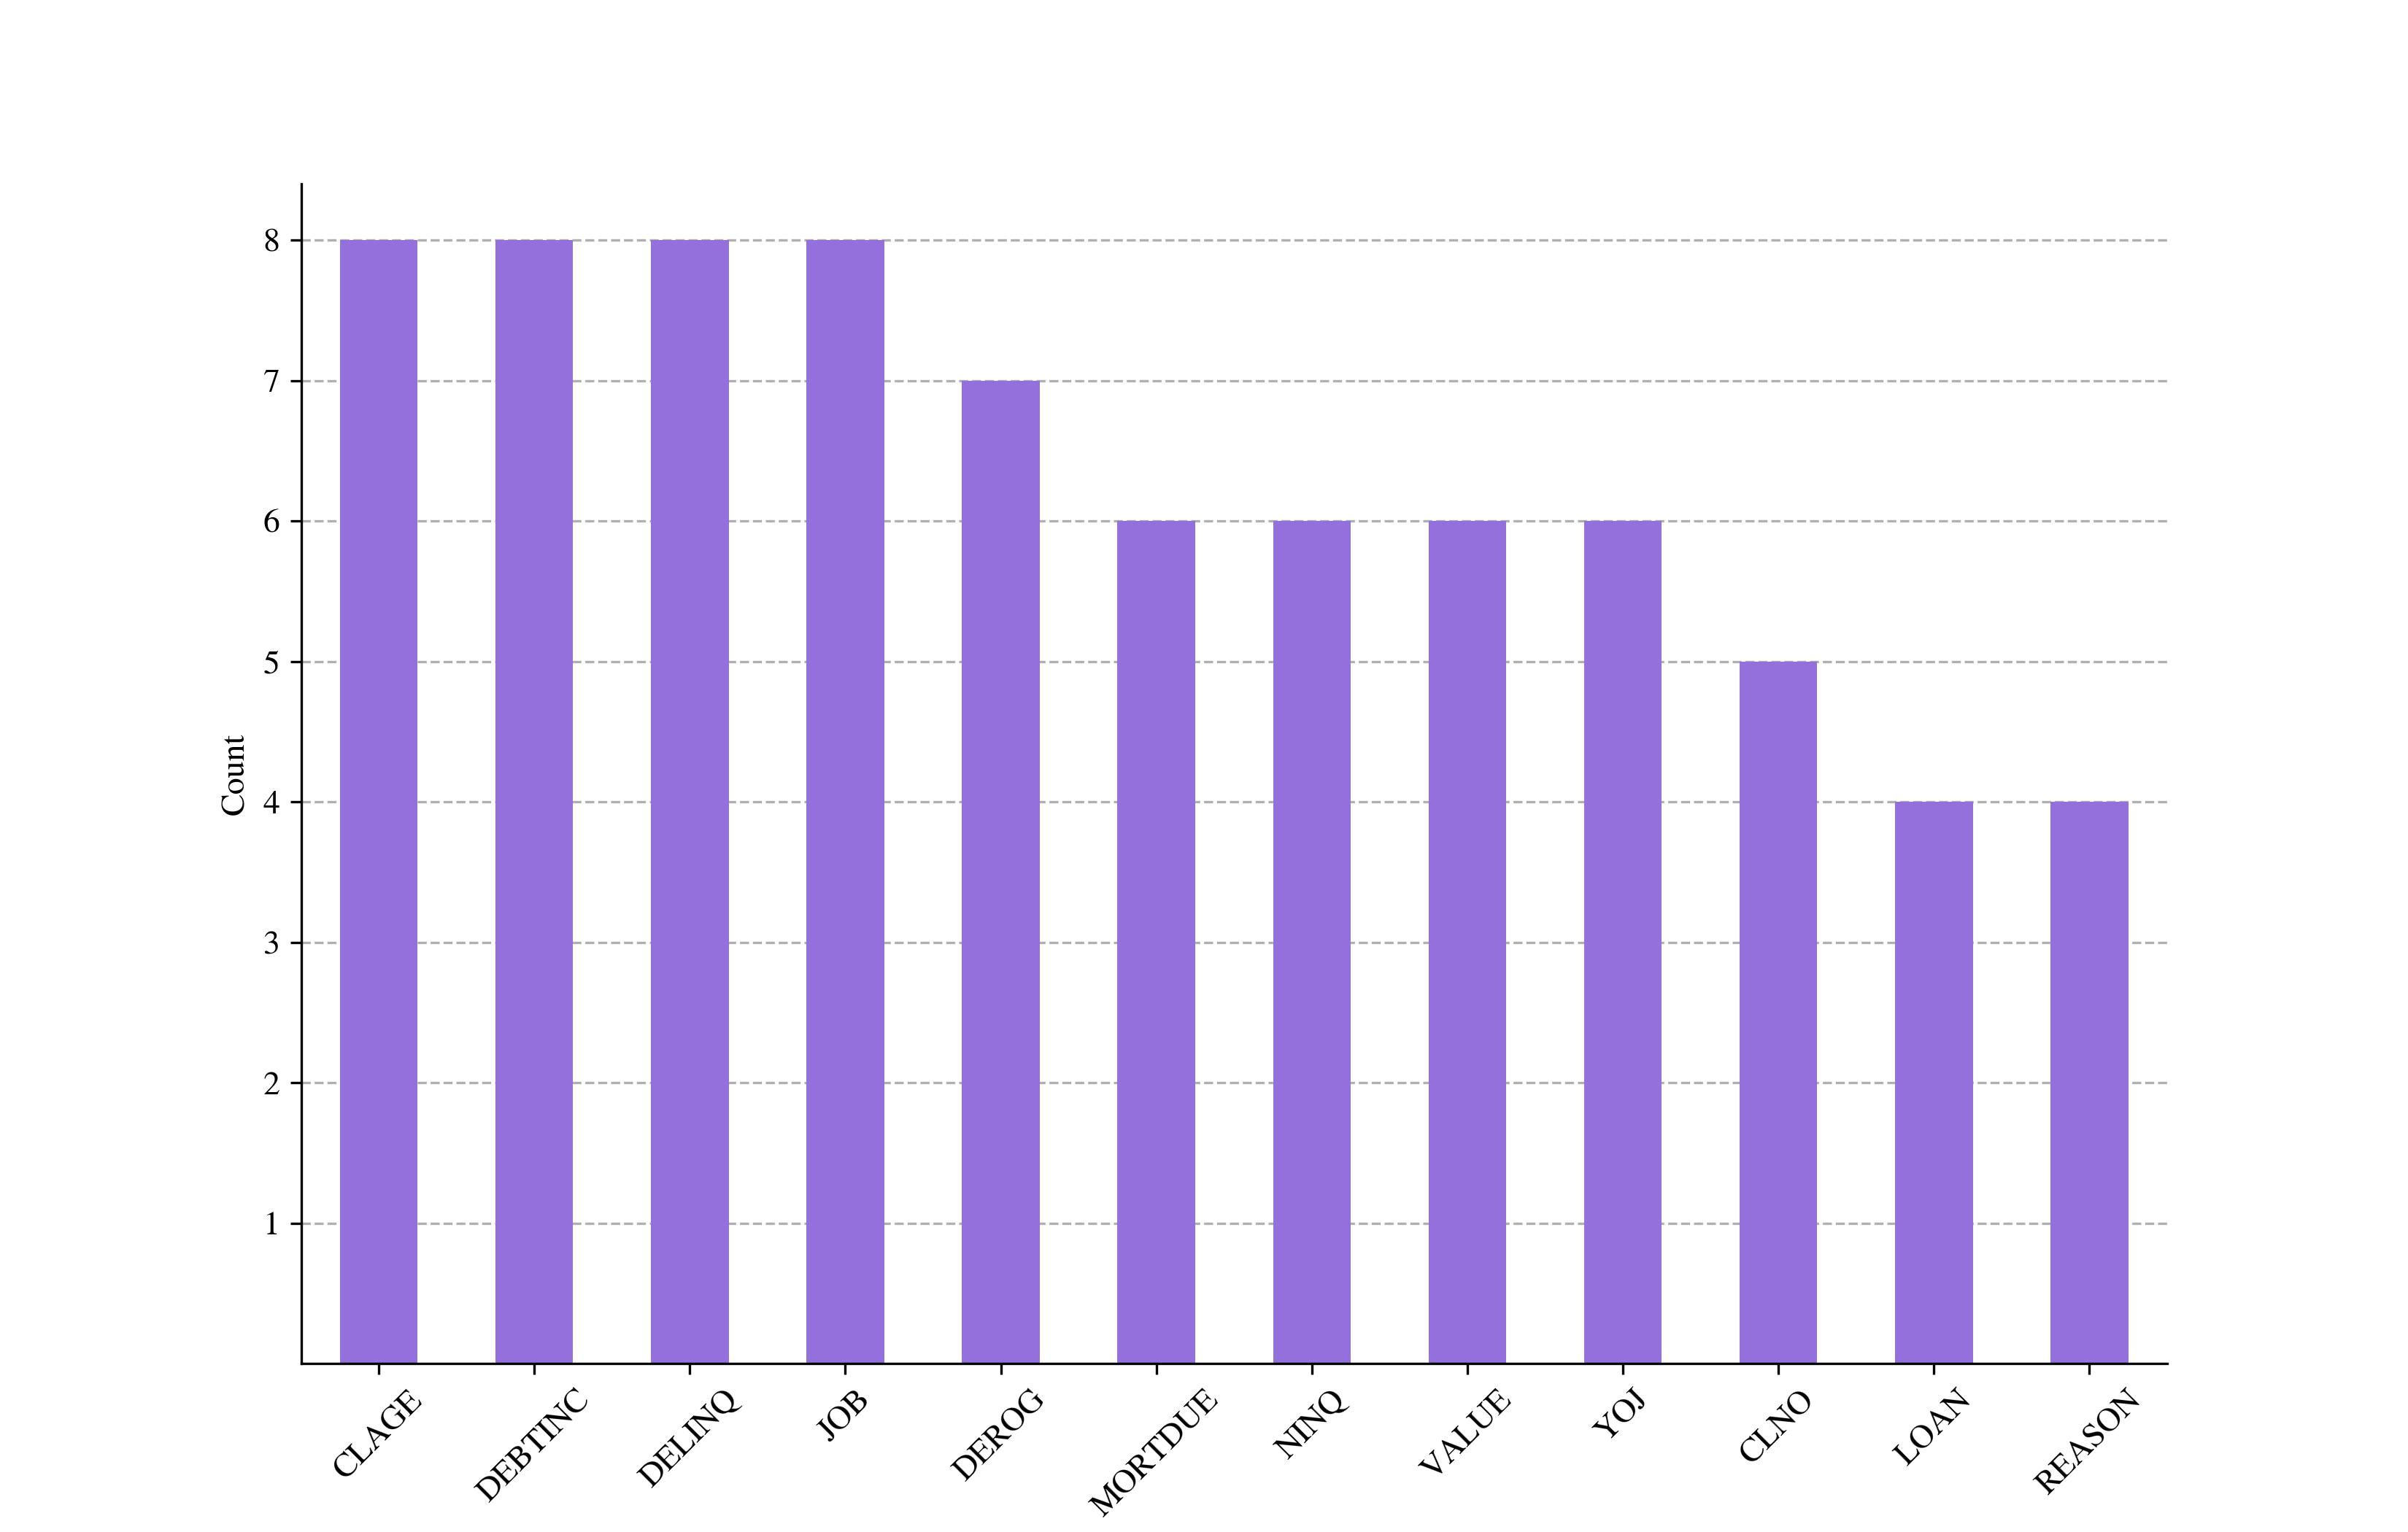
\includegraphics[width=140mm]{Figures/Recurrence_Selected_Features.jpg}
\centering{\begin{source}Author's results in Python\end{source}}\vspace{-1em}
\end{figure}


According to \autoref{fig:fsdistmod}, models such as K--Nearest Neighbors, Random Forest, Gradient Boosting and Support Vector Machine chose almost all the features as onlt one feature feature was eliminated. On the other hand, Gaussian Naive Bayes chose only 6. It seems to be that most of the features are important as each model has selected a higher amount of features.
It is evident the more comples and/or black--box models require more features in contrast to transparant models such as Logistic Regression or Gaussian Naive Bayes.

\begin{figure}[H]
    \centering
    \caption{Distribution of Selected Features per Model}\vspace{0.5em}
    \label{fig:fsdistmod}\
    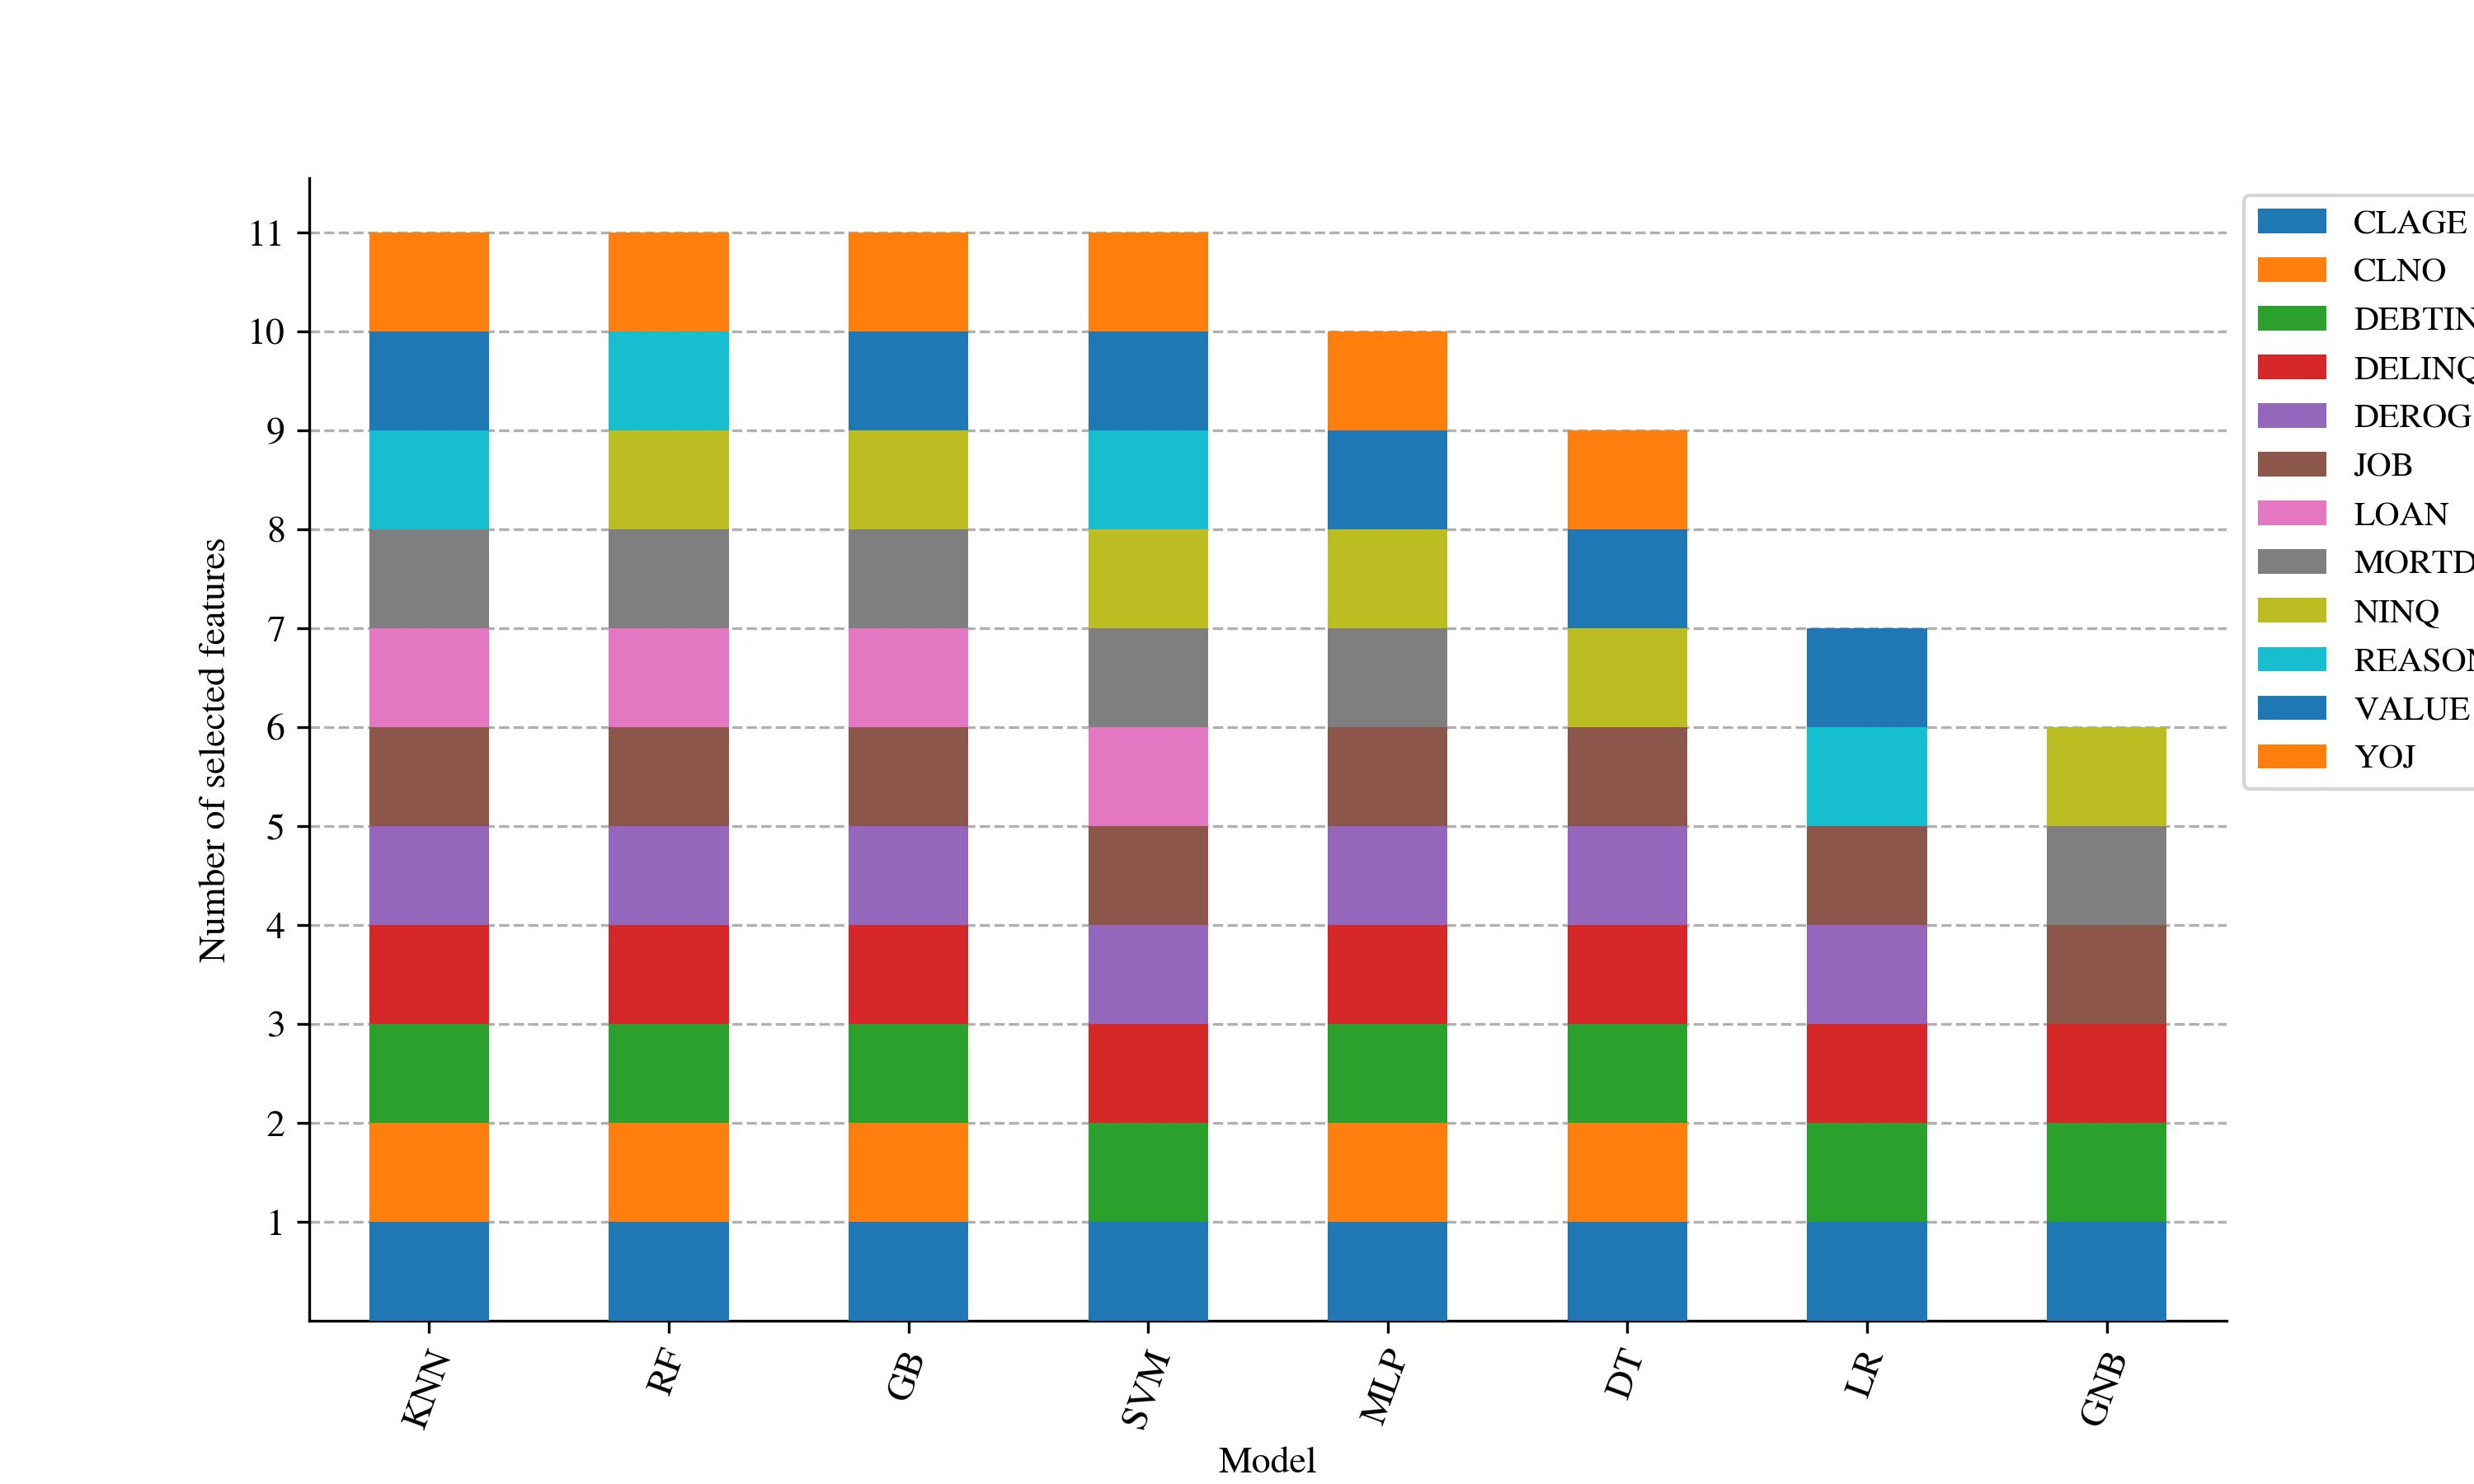
\includegraphics[width=140mm]{Figures/Selected_Features_Distribution.jpg}
    \centering{\begin{source}Author's results in Python\end{source}}\vspace{-1em}
\end{figure}

\subsection{Model Selection}

In combination with the pre--selected subsets of features, the next step regards the selection of the final model which will be further used within an evaluation and the deployment. The algorithm process is described in Algorithm  \autoref{alg:model_selection} below:
\begin{algorithm}[H]
\caption{Model Selection Algorithm}
\label{alg:model_selection}
\begin{algorithmic}[1]
\For{$model \in \textit{models}$}
    \For{$features \in \textit{features\_subsets}$}
        \State $\textit{optimized\_model} \gets \textsc{BayesianOptimization}(model, features)$
        \For{$\textit{metric} \in \textit{evaluation\_metrics}$}
            \State $\textit{performance} \gets \textsc{Evaluation}(\textit{optimized\_model}, \textit{metric})$
        \EndFor
    \EndFor
\EndFor
\end{algorithmic}
\end{algorithm}


\vspace{-1em}
Therefore, each input model is tuned on each subset of features selected within feature selection on the training set and subsequently, the optimized model is evaluated on the validation set. Thus, when having $n$ input models and $m$ subsets of selected features, we get $n \times m$ tuned models.
$m \leq n$ because we exclude duplicated subset of selected features which can occur when more than one model choose the same subset(s) of features.
Since there are 8 input models and 8 unique subsets of selected features, the total number of tuned models is 64.

\subsubsection{Metrics Space}

When evaluating classification models using class-based metrics such as F1 score, Precision, Recall, Accuracy, Matthews Correlation Coefficient, a default classification threshold of 0.5 is often used. This threshold separates predicted classes based on whether the predicted probability score is higher or lower than 0.5.
However, in real-world use cases, the 0.5 classification threshold may not be appropriate and according to \citep{esposito2021ghost}, such threshold is not appropriate when having imbalanced ata. Therefore, it is recommended to calculate an optimal threshold rather than relying on the default one.
For such case, the Youden index is employed which is derived from ROC curve and enables the selection of an optimal classification threshold value. 
The Younden index searches for the threshold that maximizes the sum of True Positive Rate and True Negative Rate, decreased by 1 \citep{fluss2005estimation}, thus:
\begin{equation}\label{eq}
J = TPR + TNR - 1
\end{equation}
Mathematically, the optimal threshold using Youden index is derived as follows:
\begin{equation}\label{eq}
T_{opt} = \text{argmax}_{t \in [0, 1]}\left(J\right)
\end{equation}
In Python, the \lstinline{roc_curve} function from \lstinline{Scikit-learn} returns False Positive Rate instead of the True Negative Rate. Nevertheless, we can derive the True Negative Rate from False Positive Rate as follows:
\begin{equation}\label{eq}
TNR =  1-FPR
\end{equation}
Therefore:
\begin{equation}\label{eq}
T_{opt} = \text{argmax}_{t \in [0, 1]}\left(TPR +  \left(1-FPR\right) - 1\right)
\end{equation}
Note, that the optimal threshold is calculated based on the training set and henceforth is applied within the evaluation on validation set.

In order to ensure a more comprehensive and unbiased evaluation of a model's performance, it is recommended to consider multiple metrics rather than relying on a single metric alone. This approach provides a more generalized overview of the model's performance across different aspects and helps to prevent any bias towards a single metric.
To accomplish this, models can be ranked based on their performance on each individual metric, where a higher score or a lower loss indicates a better model, resulting in a higher rank for that metric. Subsequently, for each metric, the ranking of the models is determined, and the final ranking is calculated as a weighted average of these individual rankings.
The weights have been set expertly and are summarized in \autoref{tab:weightsrank}.

Specifically, the highest weight (1.5) is assigned to the F1 score, which provides a balanced measure of a model's performance with respect to both False Positives and False Negatives.
This metric is commonly used in classification tasks, particularly in imbalanced data sets, such as the validation set in our case, which has not been oversampled.
In addition to the F1 score, higher weight is assigned to the Recall score as well (1.2), which is a metric that penalizes False Negatives.
False Negatives occur when the model predicts a negative result (i.e., no default) for an instance that is actually positive (i.e., default).
In the context of loan applications, one may prefer to reject a loan applicant who would not have defaulted (False Positive) rather than approving the application of a client who would have defaulted (False Negative). Therefore, it is appropriate to give higher weight to Recall in order to reduce the likelihood of False Negatives.
Henceforth, the weights are assigned to different metrics based on their relevance to the models' ranking, with the highest weight given to F1 score and additional weight given to Recall to ensure that False Negatives are minimized.

\begin{table}[H]
\small
\setlength{\tabcolsep}{8pt}
\renewcommand{\arraystretch}{1.3}
\centering
    \caption[Model Ranking Weights table]{Model Ranking Weights table}\label{tab:weightsrank}
    \begin{tabular}{>{\raggedleft\arraybackslash}p{0.4\linewidth} l}
\toprule
\textbf{Metric} & \textbf{Weight}\\
\midrule
\hline
F1 score & 1.5 \\
Recall & 1.2 \\
Precision & 1 \\
Accuracy & 1 \\
AUC & 1 \\
Somers' D & 1 \\ 
Kolmogorov Smirnov & 1 \\
Matthews Correlation Coefficient  & 1 \\
Brier Score Loss  & 1 \\
\hline
\bottomrule
\end{tabular}
\vspace{0.7em}

\centering{\begin{source}Author's results in Python\end{source}}\vspace{-1em}
\end{table}

Particularly, for each model a rank score is calculated in order to determine the final rank. The lower rank score indicates better model performance. For particular model $M$, the rank score as weighted sum of the individual ranks as follows:
\begin{equation}\label{eq:rankscorem}
    RankScore_{M} = \frac{\sum_{i=1}^{k} {r_i \times w_i}}{\sum_{i=1}^{k} {w_i}} 
\end{equation}
where $k$ is the number of metrics used to evaluated the model $M$, $r_i$ is the rank order of $i$--th metric for given model $M$ and $w_i$ is the weight assigned to the $i$--th metric.
Such metric lies in interval $<1, k>$, where 1 would indicate a perfect model performance across the all metrics.

\textbf{QUESTION: Should we also add this metric for better interpretability or is the metric defined above sufficient?}

For better interpretability, we can normalize the rank scores which would range from 0 to 1 where 1 would indicate a perfect performance of the model.
\begin{equation}\label{eq}
    NormRankScore_{M} = 1 - \frac{RankScore_{M} - k}{k - 1}
\end{equation}

\subsubsection{Model Selection Results}



The custom function \lstinline{model_selection()} iteratively prints the process of the model tuning and evaluation on each subset of features, in order to keep the track of such process as it is depicted in \autoref{fig:modselprint}.
Particularly, it prints which model on which features is being tuned and evaluated, exeuction time, optimal threshold, F1 score on the validation set and the best hyperparameters.

\begin{figure}[H]
\centering\caption{Model Selection Print Statement}
\label{fig:modselprint}

{\fontsize{8.8}{11}\selectfont 
\begin{verbatim}
-------------------------------------------------------------------------------------
--------------------------------------- 56/64 ---------------------------------------
-------------------------------------------------------------------------------------
---------------------------- BAYESIAN OPTIMIZATION OF SVM ---------------------------
--------------------------- WITH FEATURES SELECTED BY MLP ---------------------------
-------------------------------------------------------------------------------------
------------------------------------------------------------------------------------- 

1/2 ... Starting Bayesian Optimization on the subset of features (10 features):
        MORTDUE, VALUE, JOB, YOJ, DEROG, DELINQ, CLAGE, NINQ, CLNO, DEBTINC
2/2... Bayesian Optimization finished 

Execution time: 22.0695 minutes 

F1 Score on Validation set: 0.7102272727272726 

Optimal classification threshold: 0.6477 

Tuned hyperparameters of SVM: 

    C: 4.999999999999999
    break_ties: False
    cache_size: 200
    class_weight: balanced
    coef0: 0.0
    decision_function_shape: ovr
    degree: 1
    gamma: scale
    kernel: rbf
    max_iter: -1
    probability: True
    random_state: 42
    shrinking: False
    tol: 1.102507160381566e-09
    verbose: False

-------------------------------------------------------------------------------------
------------------------------------------------------------------------------------- 
\end{verbatim}
}
\centering{\begin{source}Author's results in Python\end{source}}\vspace{0em}
\end{figure}



The final output of the function \lstinline{model_selection()} is table which summarizes the model's computed metrics as depicted in \autoref{tab:modelsectab}. As can be seen, the best models in terms of ranking are the Gradient Boosting models which in general have the highest score metrics and the lowest loss metrics. On the other hand, the worst-performing models are Gaussian Naive Bayes models.


\clearpage
\newpage

\KOMAoptions{paper=landscape,DIV=last}
\newgeometry{hmargin=2.5cm,bottom=25mm,height=150mm,includehead}
\fancyheadoffset{0pt}



\begin{table}[H]
\small
\setlength{\tabcolsep}{8pt}
\renewcommand{\arraystretch}{1.3}
\caption[Model Selection table]{Model Selection Results}\label{tab:modelsectab}
\centering
\scalebox{0.8}{

\begin{tabular}{|p{1.3cm}|p{1.2cm}|p{1.4cm}|r|c|c|c|c|c|c|c|c|c|c|c|c|c||c|c|}
    \toprule
    \textbf{Tuned model} & \textbf{FS model} & \# \newline Features & Time & Thres & F1 & Prec & Rec & Acc & AUC & SD & KS & MCC & JC & BS & Log Loss & Score & Rank \\
    \midrule
    \hline
GB & MLP & 10 & 738.19 & 0.4955 & 0.7809 & 0.7853 & 0.7765 & 0.9128 & 0.9515 & 0.9030 & 0.7751 & 0.7265 & 0.6406 & 0.0666 & 0.2487 & 3.48 & 1 \\ 
GB & KNN & 11 & 767.90 & 0.5072 & 0.7978 & 0.7912 & 0.8045 & 0.9184 & 0.9587 & 0.9175 & 0.7989 & 0.7467 & 0.6636 & 0.0687 & 0.4135 & 3.82 & 2 \\ 
GB & SVM & 11 & 904.84 & 0.5053 & 0.7896 & 0.8155 & 0.7654 & 0.9184 & 0.9555 & 0.9109 & 0.7961 & 0.7397 & 0.6524 & 0.0718 & 0.3486 & 4.17 & 3 \\ 
GB & GB & 11 & 686.26 & 0.4132 & 0.7799 & 0.7778 & 0.7821 & 0.9117 & 0.9543 & 0.9086 & 0.7989 & 0.7247 & 0.6393 & 0.0703 & 0.3372 & 4.29 & 4 \\ 
GB & RF & 11 & 802.55 & 0.4973 & 0.7775 & 0.7841 & 0.7710 & 0.9117 & 0.9541 & 0.9081 & 0.7961 & 0.7225 & 0.6359 & 0.0669 & 0.2803 & 4.37 & 5 \\ 
RF & KNN & 11 & 356.24 & 0.4725 & 0.7486 & 0.7326 & 0.7654 & 0.8972 & 0.9226 & 0.8452 & 0.7109 & 0.6843 & 0.5983 & 0.0923 & 0.3232 & 8.66 & 6 \\ 
GB & DT & 9 & 719.92 & 0.4729 & 0.7675 & 0.7697 & 0.7654 & 0.9073 & 0.9407 & 0.8814 & 0.7556 & 0.7096 & 0.6227 & 0.0808 & 0.4693 & 8.87 & 7 \\ 
RF & GB & 11 & 310.63 & 0.4517 & 0.7385 & 0.7135 & 0.7654 & 0.8916 & 0.9200 & 0.8400 & 0.7123 & 0.6709 & 0.5855 & 0.0886 & 0.3135 & 9.47 & 8 \\ 
RF & MLP & 10 & 397.42 & 0.4761 & 0.7357 & 0.7181 & 0.7542 & 0.8916 & 0.9179 & 0.8358 & 0.7081 & 0.6679 & 0.5819 & 0.0879 & 0.3084 & 10.39 & 9 \\ 
GB & LR & 7 & 1008.69 & 0.4362 & 0.7388 & 0.7000 & 0.7821 & 0.8894 & 0.9219 & 0.8438 & 0.7081 & 0.6706 & 0.5858 & 0.0886 & 0.3925 & 10.79 & 10 \\ 
\ldots & \ldots & \ldots & \ldots & \ldots & \ldots & \ldots & \ldots & \ldots & \ldots & \ldots & \ldots & \ldots & \ldots & \ldots & \ldots & \ldots & \ldots \\
DT & MLP & 10 & 54.19 & 0.5000 & 0.6427 & 0.6374 & 0.6480 & 0.8559 & 0.8133 & 0.6266 & 0.5810 & 0.5524 & 0.4735 & 0.1254 & 2.0008 & 50.38 & 55 \\ 
GNB & GB & 11 & 23.04 & 0.1829 & 0.5970 & 0.4893 & 0.7654 & 0.7933 & 0.8531 & 0.7063 & 0.5810 & 0.4880 & 0.4255 & 0.1310 & 0.6461 & 50.50 & 56 \\ 
GNB & KNN & 11 & 22.98 & 0.3588 & 0.6093 & 0.5219 & 0.7318 & 0.8123 & 0.8479 & 0.6957 & 0.5698 & 0.5024 & 0.4381 & 0.1367 & 0.6686 & 50.81 & 57 \\ 
GNB & DT & 9 & 23.11 & 0.2241 & 0.6063 & 0.5095 & 0.7486 & 0.8056 & 0.8467 & 0.6935 & 0.5768 & 0.4991 & 0.4351 & 0.1316 & 0.6370 & 50.85 & 58 \\ 
GNB & MLP & 10 & 23.11 & 0.2194 & 0.6013 & 0.5000 & 0.7542 & 0.8000 & 0.8493 & 0.6986 & 0.5768 & 0.4930 & 0.4299 & 0.1319 & 0.6360 & 50.99 & 59 \\ 
DT & GNB & 6 & 53.14 & 0.5000 & 0.6354 & 0.6284 & 0.6425 & 0.8525 & 0.8187 & 0.6375 & 0.5838 & 0.5430 & 0.4656 & 0.1251 & 2.1679 & 51.74 & 60 \\ 
GNB & GNB & 6 & 23.05 & 0.4787 & 0.5950 & 0.5039 & 0.7263 & 0.8022 & 0.8356 & 0.6711 & 0.5559 & 0.4835 & 0.4235 & 0.1470 & 0.5280 & 54.53 & 61 \\ 
LR & GNB & 6 & 95.14 & 0.4561 & 0.5948 & 0.5121 & 0.7095 & 0.8067 & 0.8379 & 0.6758 & 0.5531 & 0.4831 & 0.4233 & 0.1319 & 0.4180 & 54.97 & 62 \\ 
GNB & SVM & 11 & 22.91 & 0.1991 & 0.5885 & 0.4872 & 0.7430 & 0.7922 & 0.8425 & 0.6850 & 0.5712 & 0.4756 & 0.4169 & 0.1345 & 0.6721 & 55.15 & 63 \\ 
GNB & RF & 11 & 23.25 & 0.3413 & 0.5864 & 0.4943 & 0.7207 & 0.7966 & 0.8288 & 0.6577 & 0.5545 & 0.4720 & 0.4148 & 0.1486 & 0.7040 & 57.85 & 64 \\ 
    \hline
    \bottomrule 
\end{tabular}}
\vspace{1em}

\centering{\begin{source}Author's results in Python\end{source}}\vspace{-1em}
\end{table}

\clearpage
\newpage
\KOMAoptions{paper=portrait,DIV=last}
\restoregeometry
\fancyheadoffset{0pt}

In order to gain a more detailed understanding of the model selection results, the distribution of computed metrics is plotted. In \autoref{fig:f1dist}, the F1 score distribution is visualized for each input model. An outlier can be observed in KNN where the F1 score is 0.				
\begin{figure}[H]
\centering
\caption{F1 score distribution}\vspace{0.5em}
\label{fig:f1dist}\
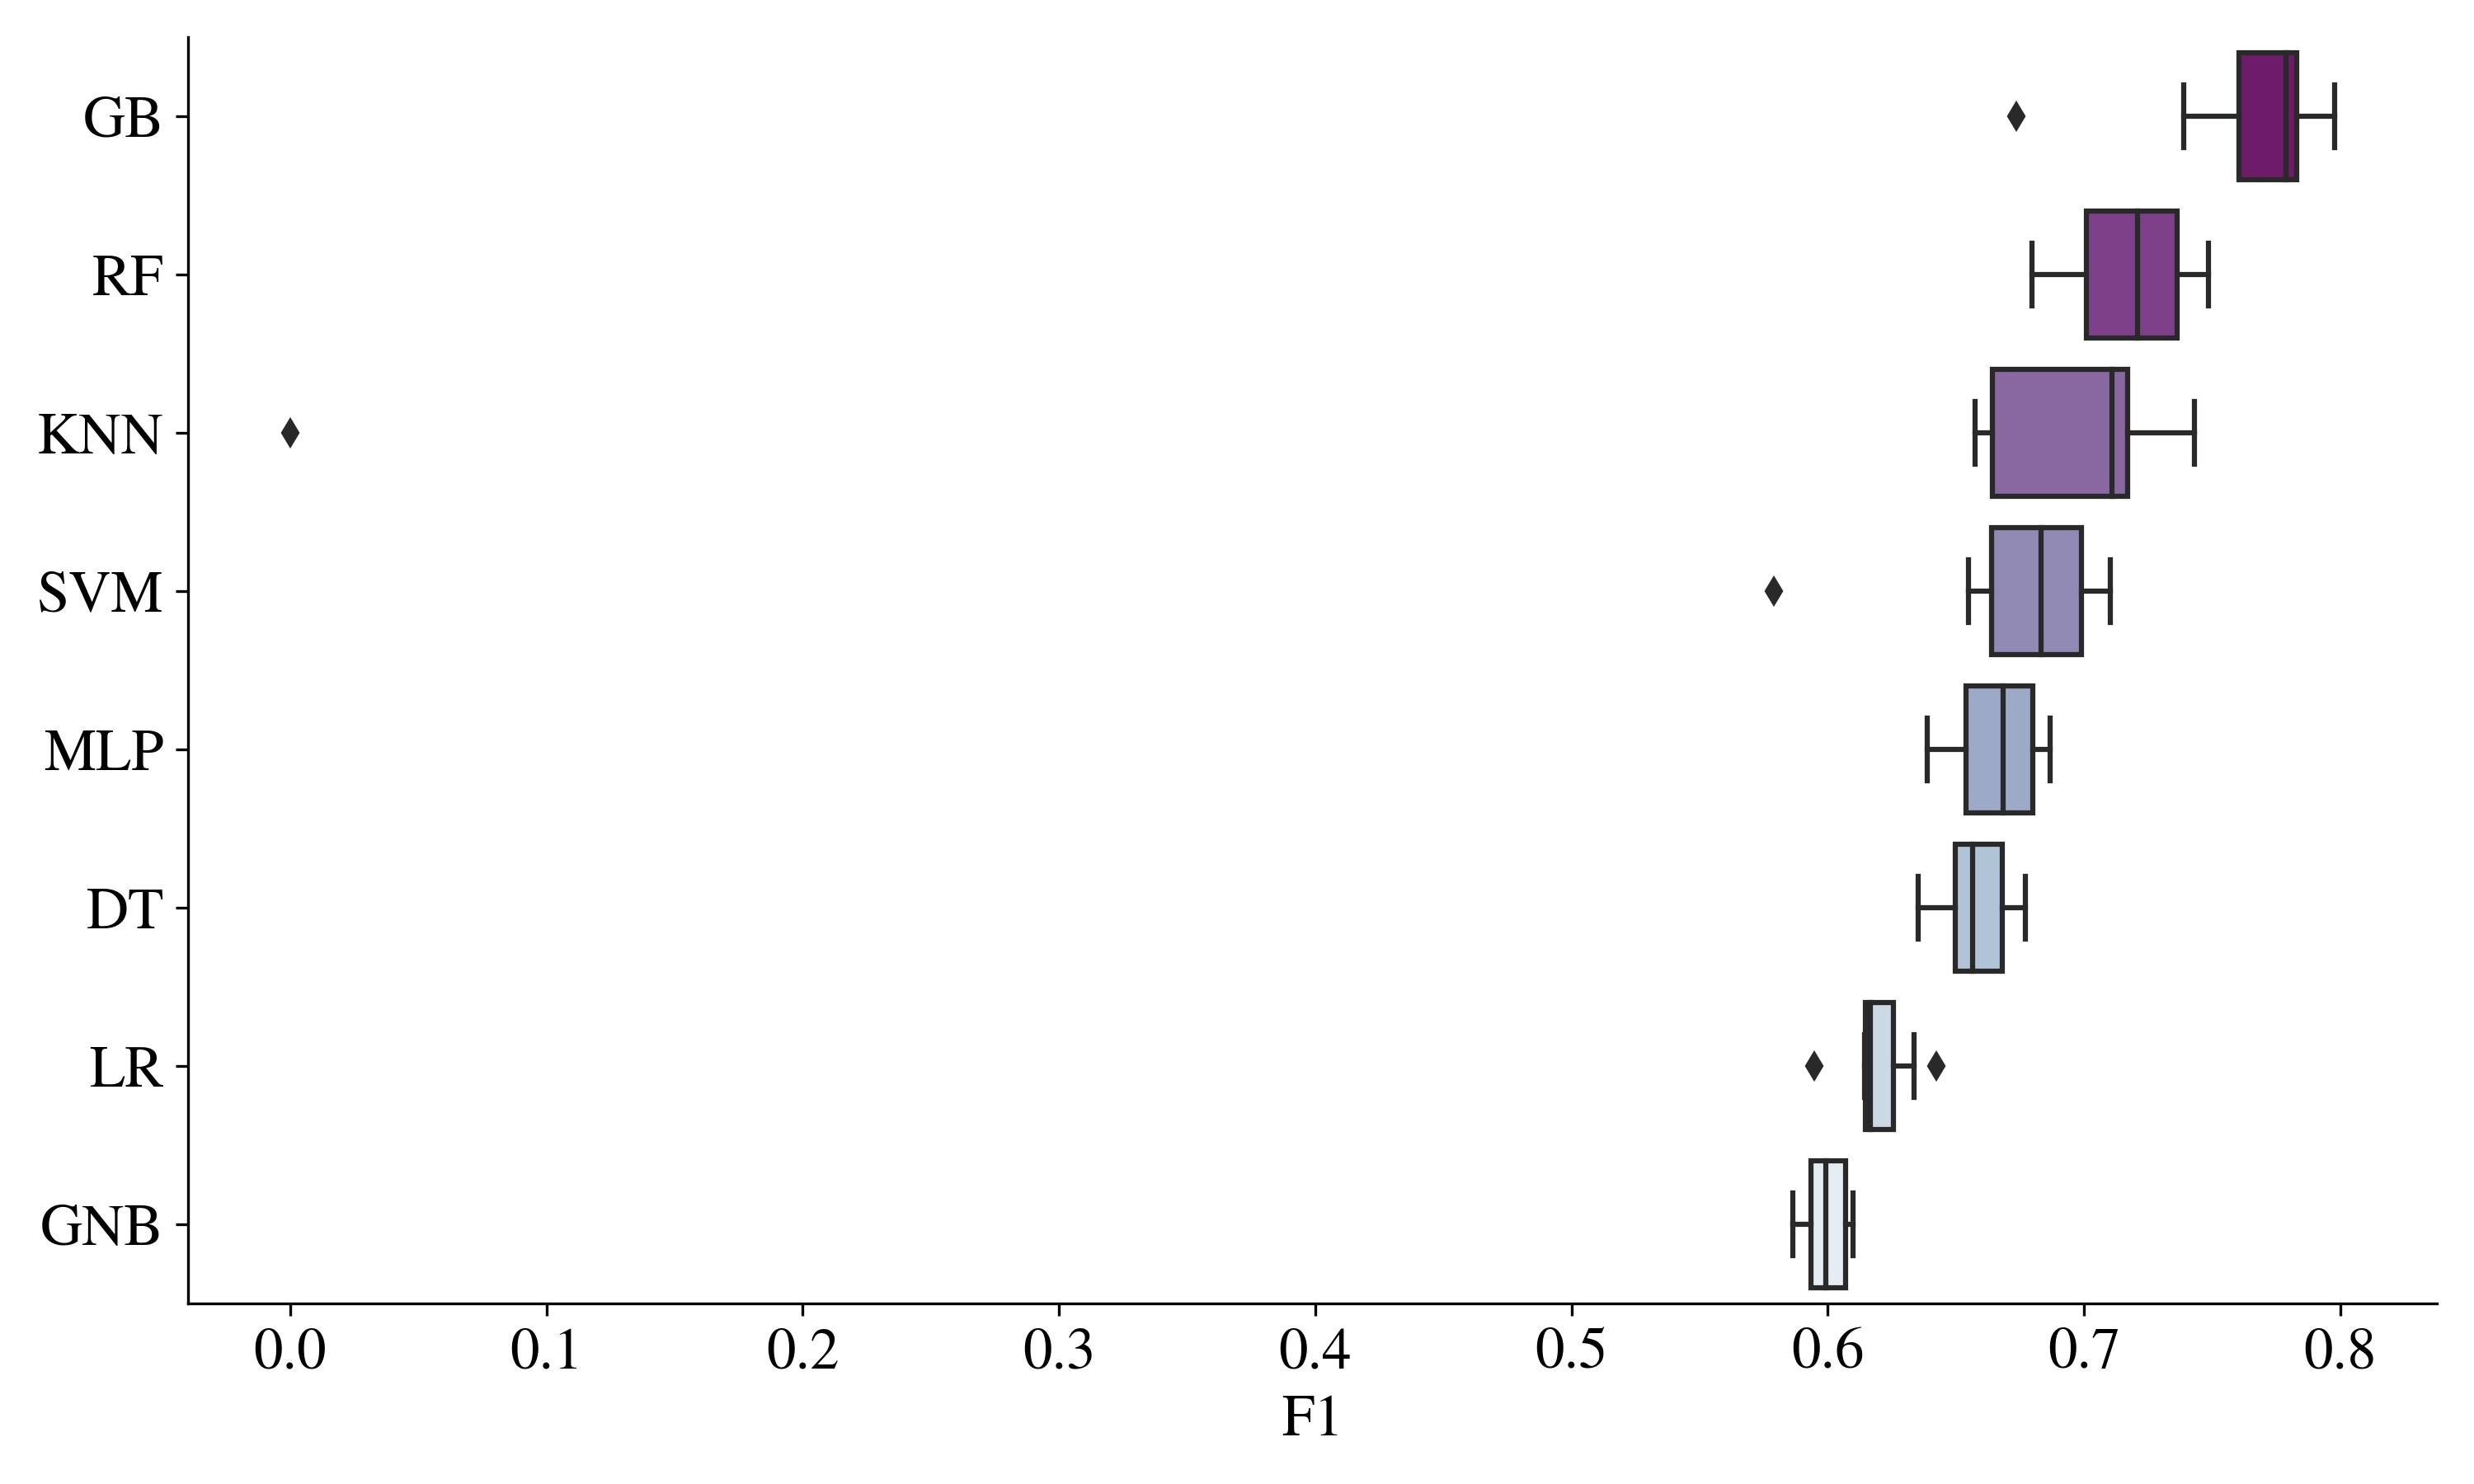
\includegraphics[width=140mm]{Figures/F1_Distribution.jpg}
\centering{\begin{source}Author's results in Python\end{source}}\vspace{-1em}
\end{figure}
Such outlier is removed in \autoref{fig:f1distclean} to gain a more general insight into the F1 score distribution.
It can be observed that Gradient Boosting models have the highest F1 scores of around 80 \%.
Another tree ensemble model, Random Forest, is performing well as the second best. However, more transparent models such as Logistic Regression and Naive Bayes are performing poorly, having F1 scores around 60 \%.
Surprisingly, black box models such as Support Vector Machine and Neural Network are outperformed by the less complex KNN model.
Nonetheless, given the relatively small sample size, KNN performs better than Neural Network and non-linear SVM on small data sets.
\begin{figure}[H]
\centering
\caption{F1 score distribution - without outlier}\vspace{0.5em}
\label{fig:f1distclean}\
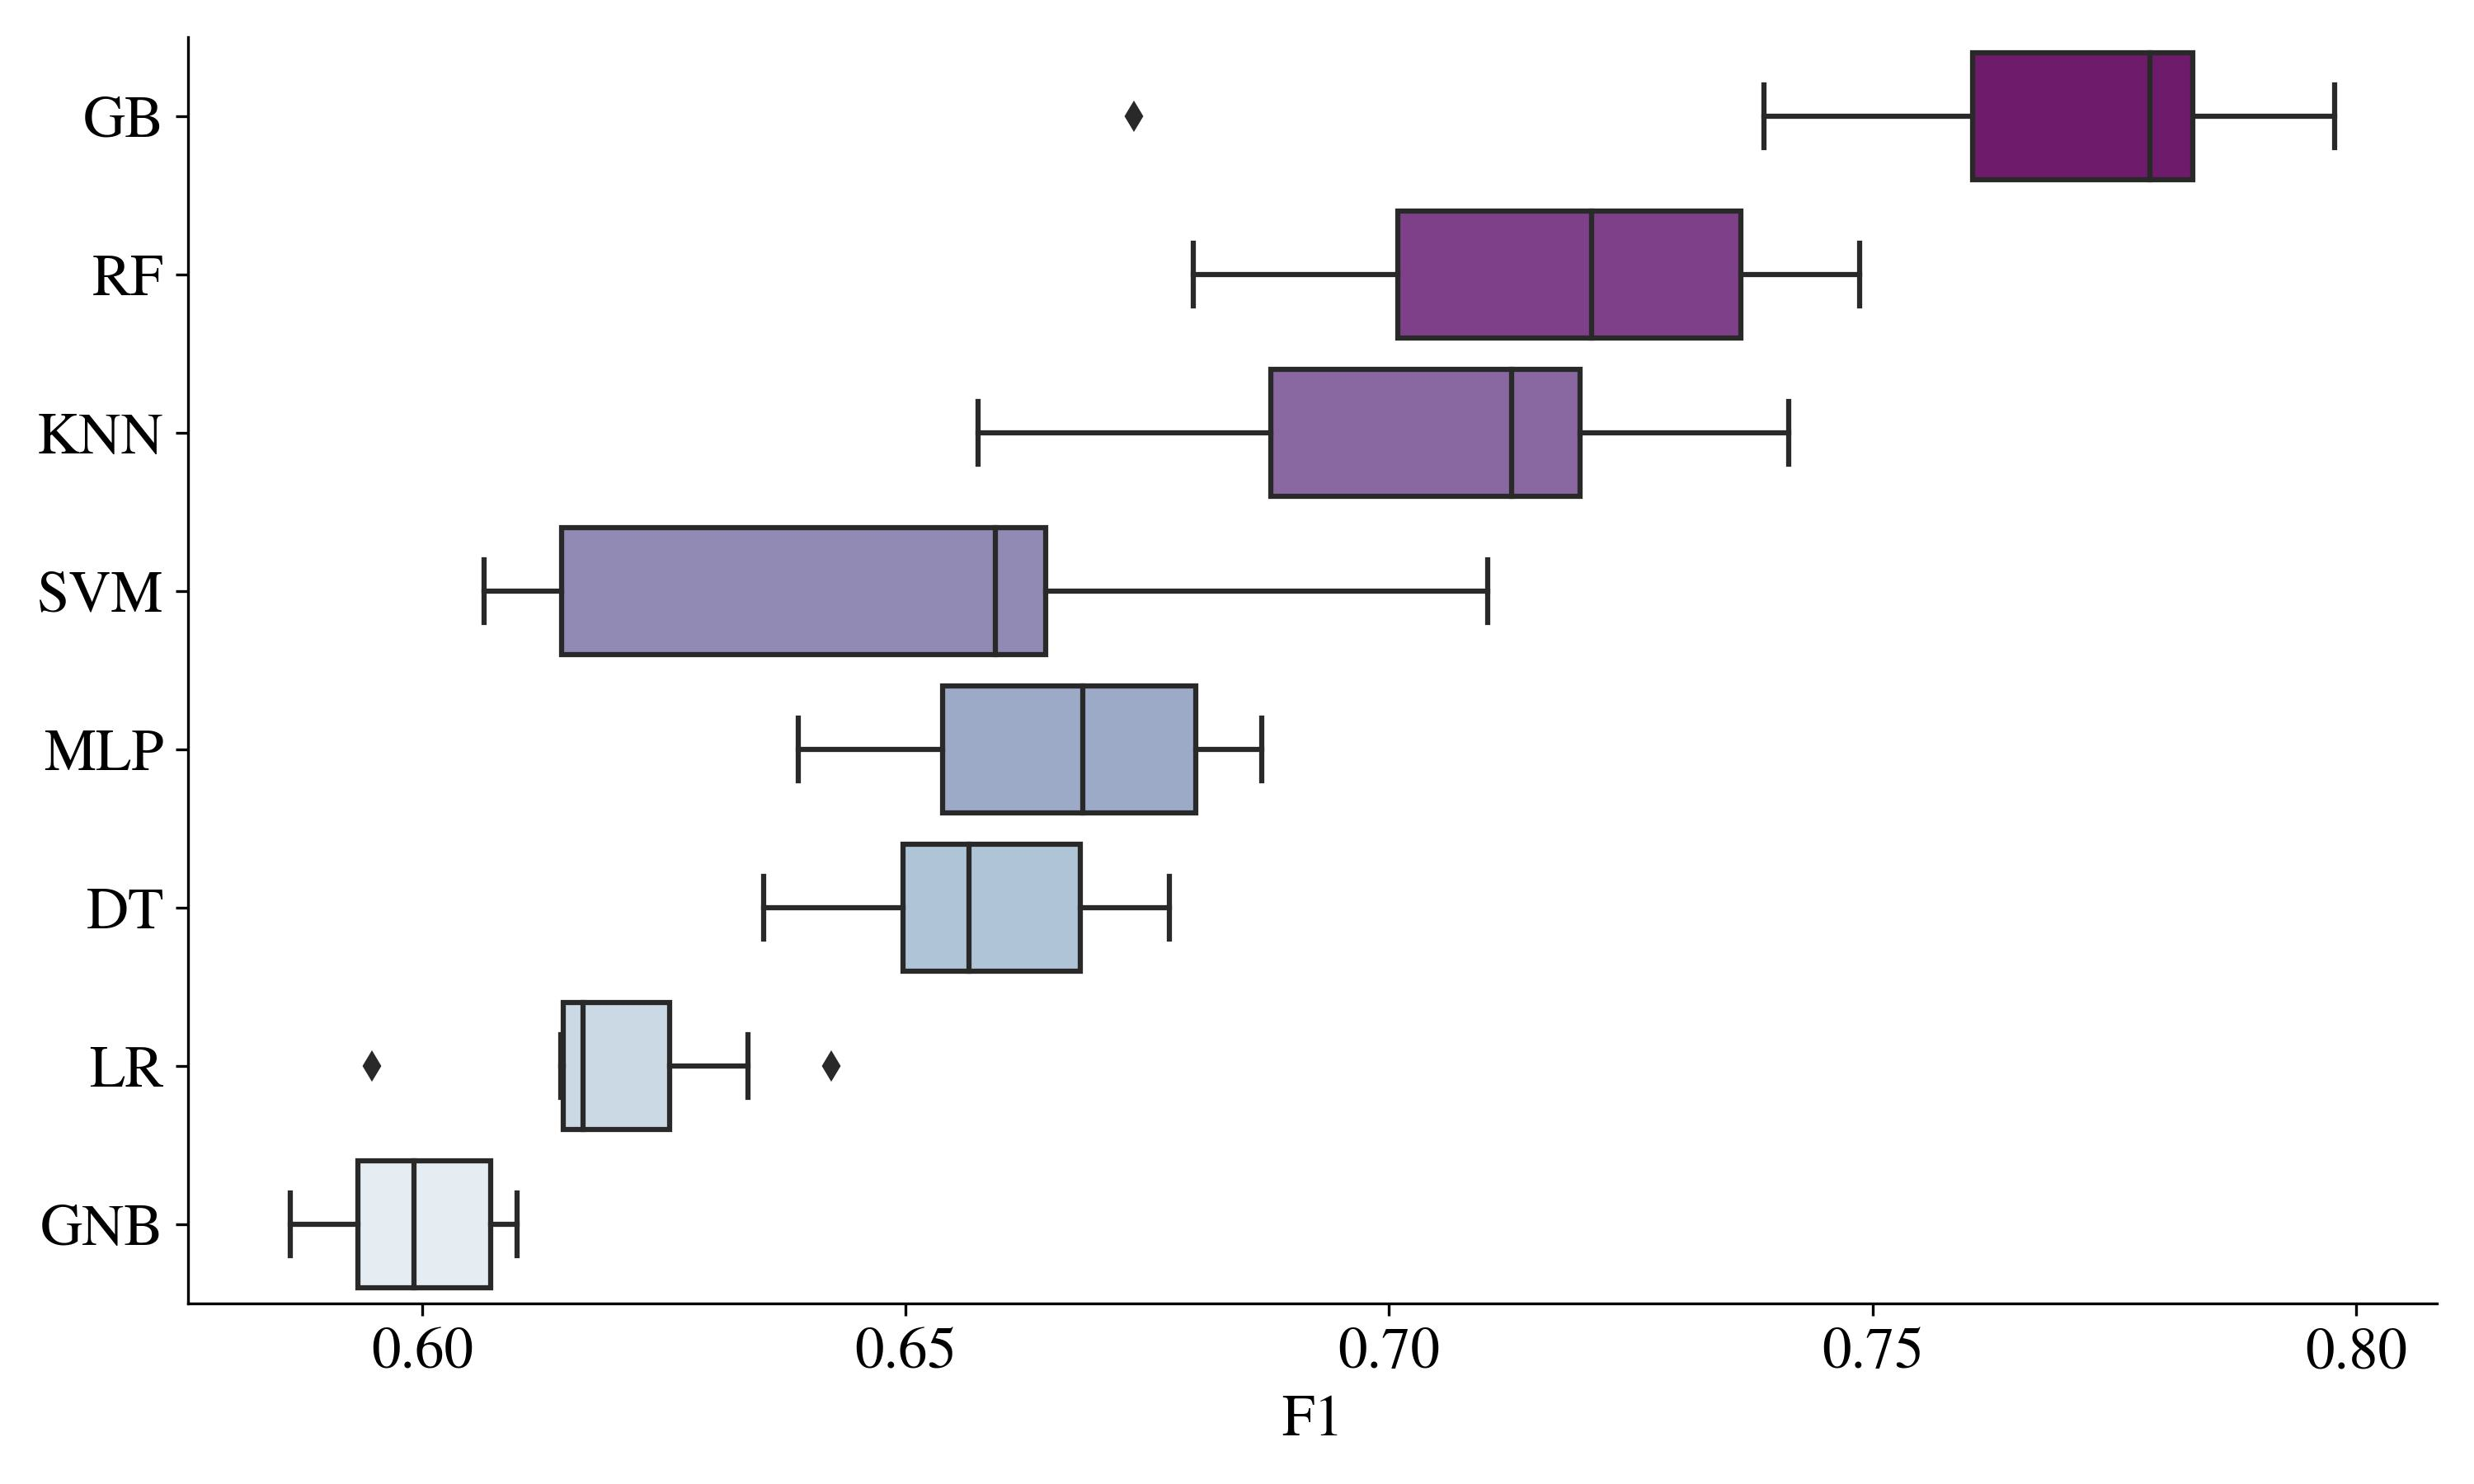
\includegraphics[width=140mm]{Figures/F1_wo_outliers_Distribution.jpg}
\centering{\begin{source}Author's results in Python\end{source}}\vspace{-1em}
\end{figure}

As depicted in \autoref{fig:f1distcleanbbwb}, the distribution of F1 score (without the outlier) across the model type. Although, both score distributions overlap, it is evident, that black--box models outperform white--box model in terms of F1 score in overall as expected.
\begin{figure}[H]
    \centering
    \caption{F1 score distribution (Black--box/White--box dimension) - without outlier}\vspace{0.5em}
    \label{fig:f1distcleanbbwb}\
    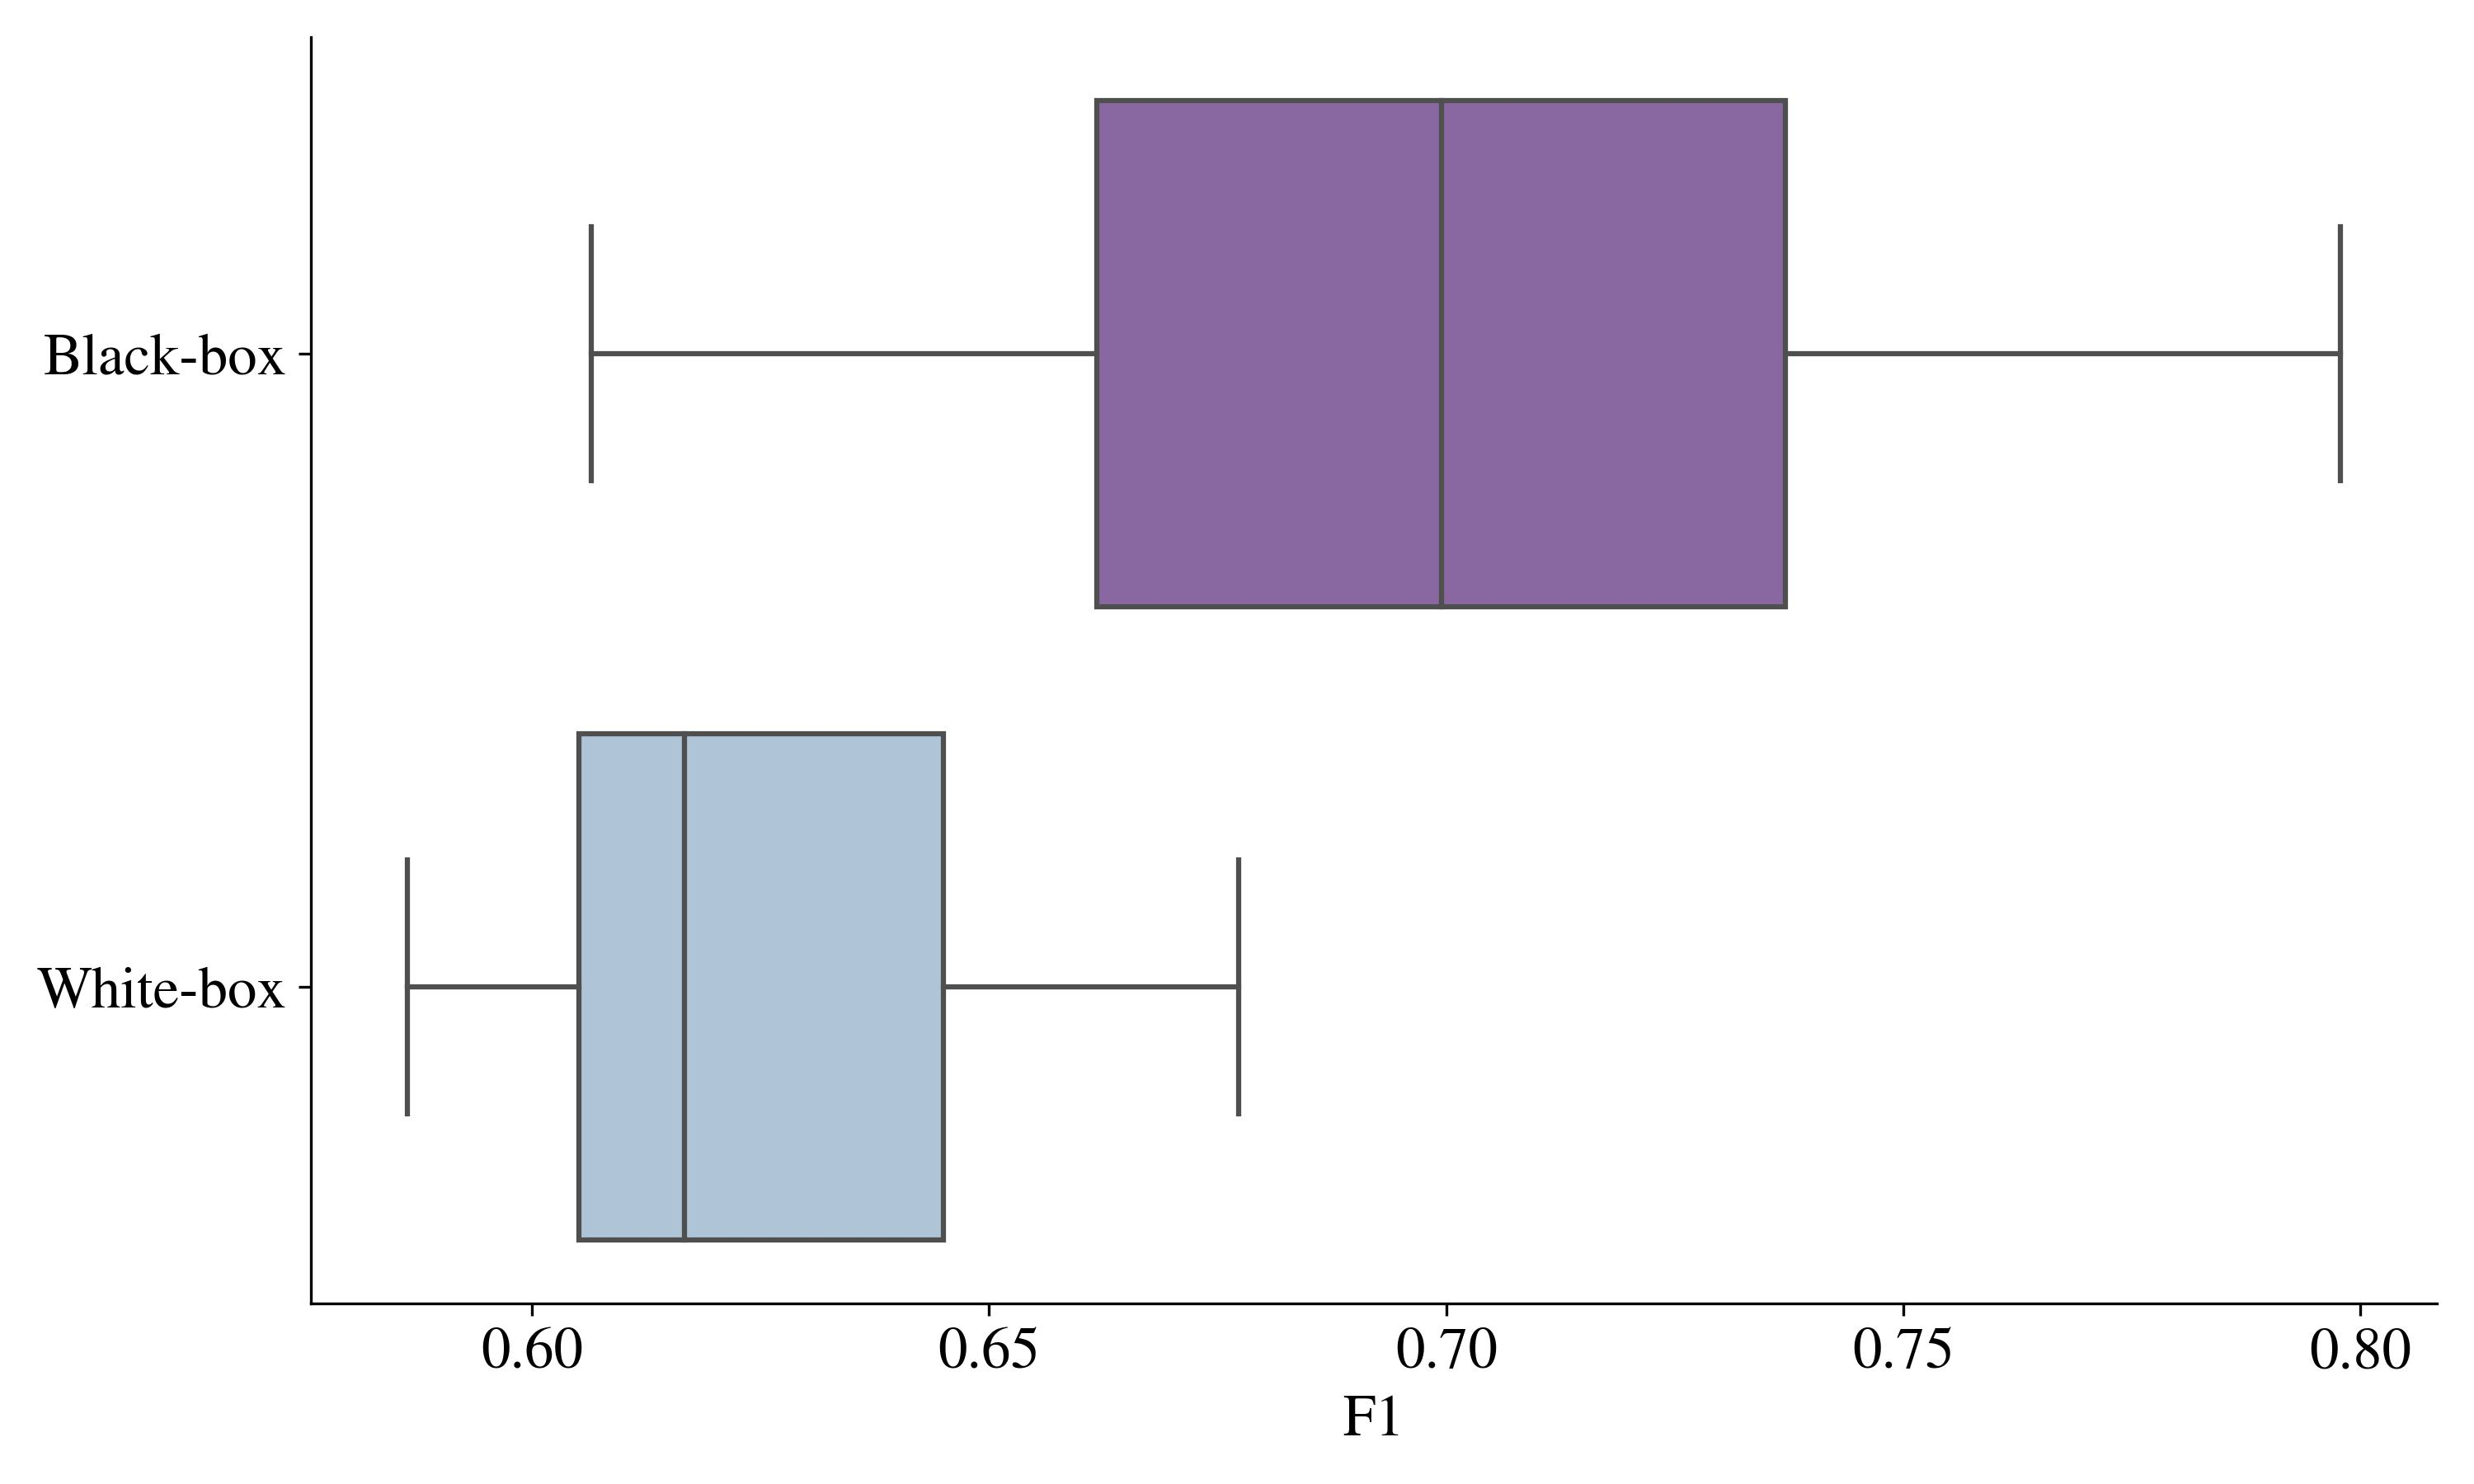
\includegraphics[width=140mm]{Figures/F1_wo_outliers_Distribution_BB_WB.jpg}
    \centering{\begin{source}Author's results in Python\end{source}}\vspace{-1em}
\end{figure}

We can also consider not only F1 score but also other metrics, which is quantified in the rank score calculated according to \autoref{eq:rankscorem}. As shown in \autoref{fig:avgrankdist}, we can observe that the order of models ranked by the rank score is identical as the order of the models ranked by F1 score in \autoref{fig:f1dist}.
Hence, across all the metrics, the Gradient Boosting perform the best in overall while Gaussian Naive Bayes do not perform well at all.
\begin{figure}[H]
    \centering
    \caption{Rank Score distribution}\vspace{0.5em}
    \label{fig:avgrankdist}\
    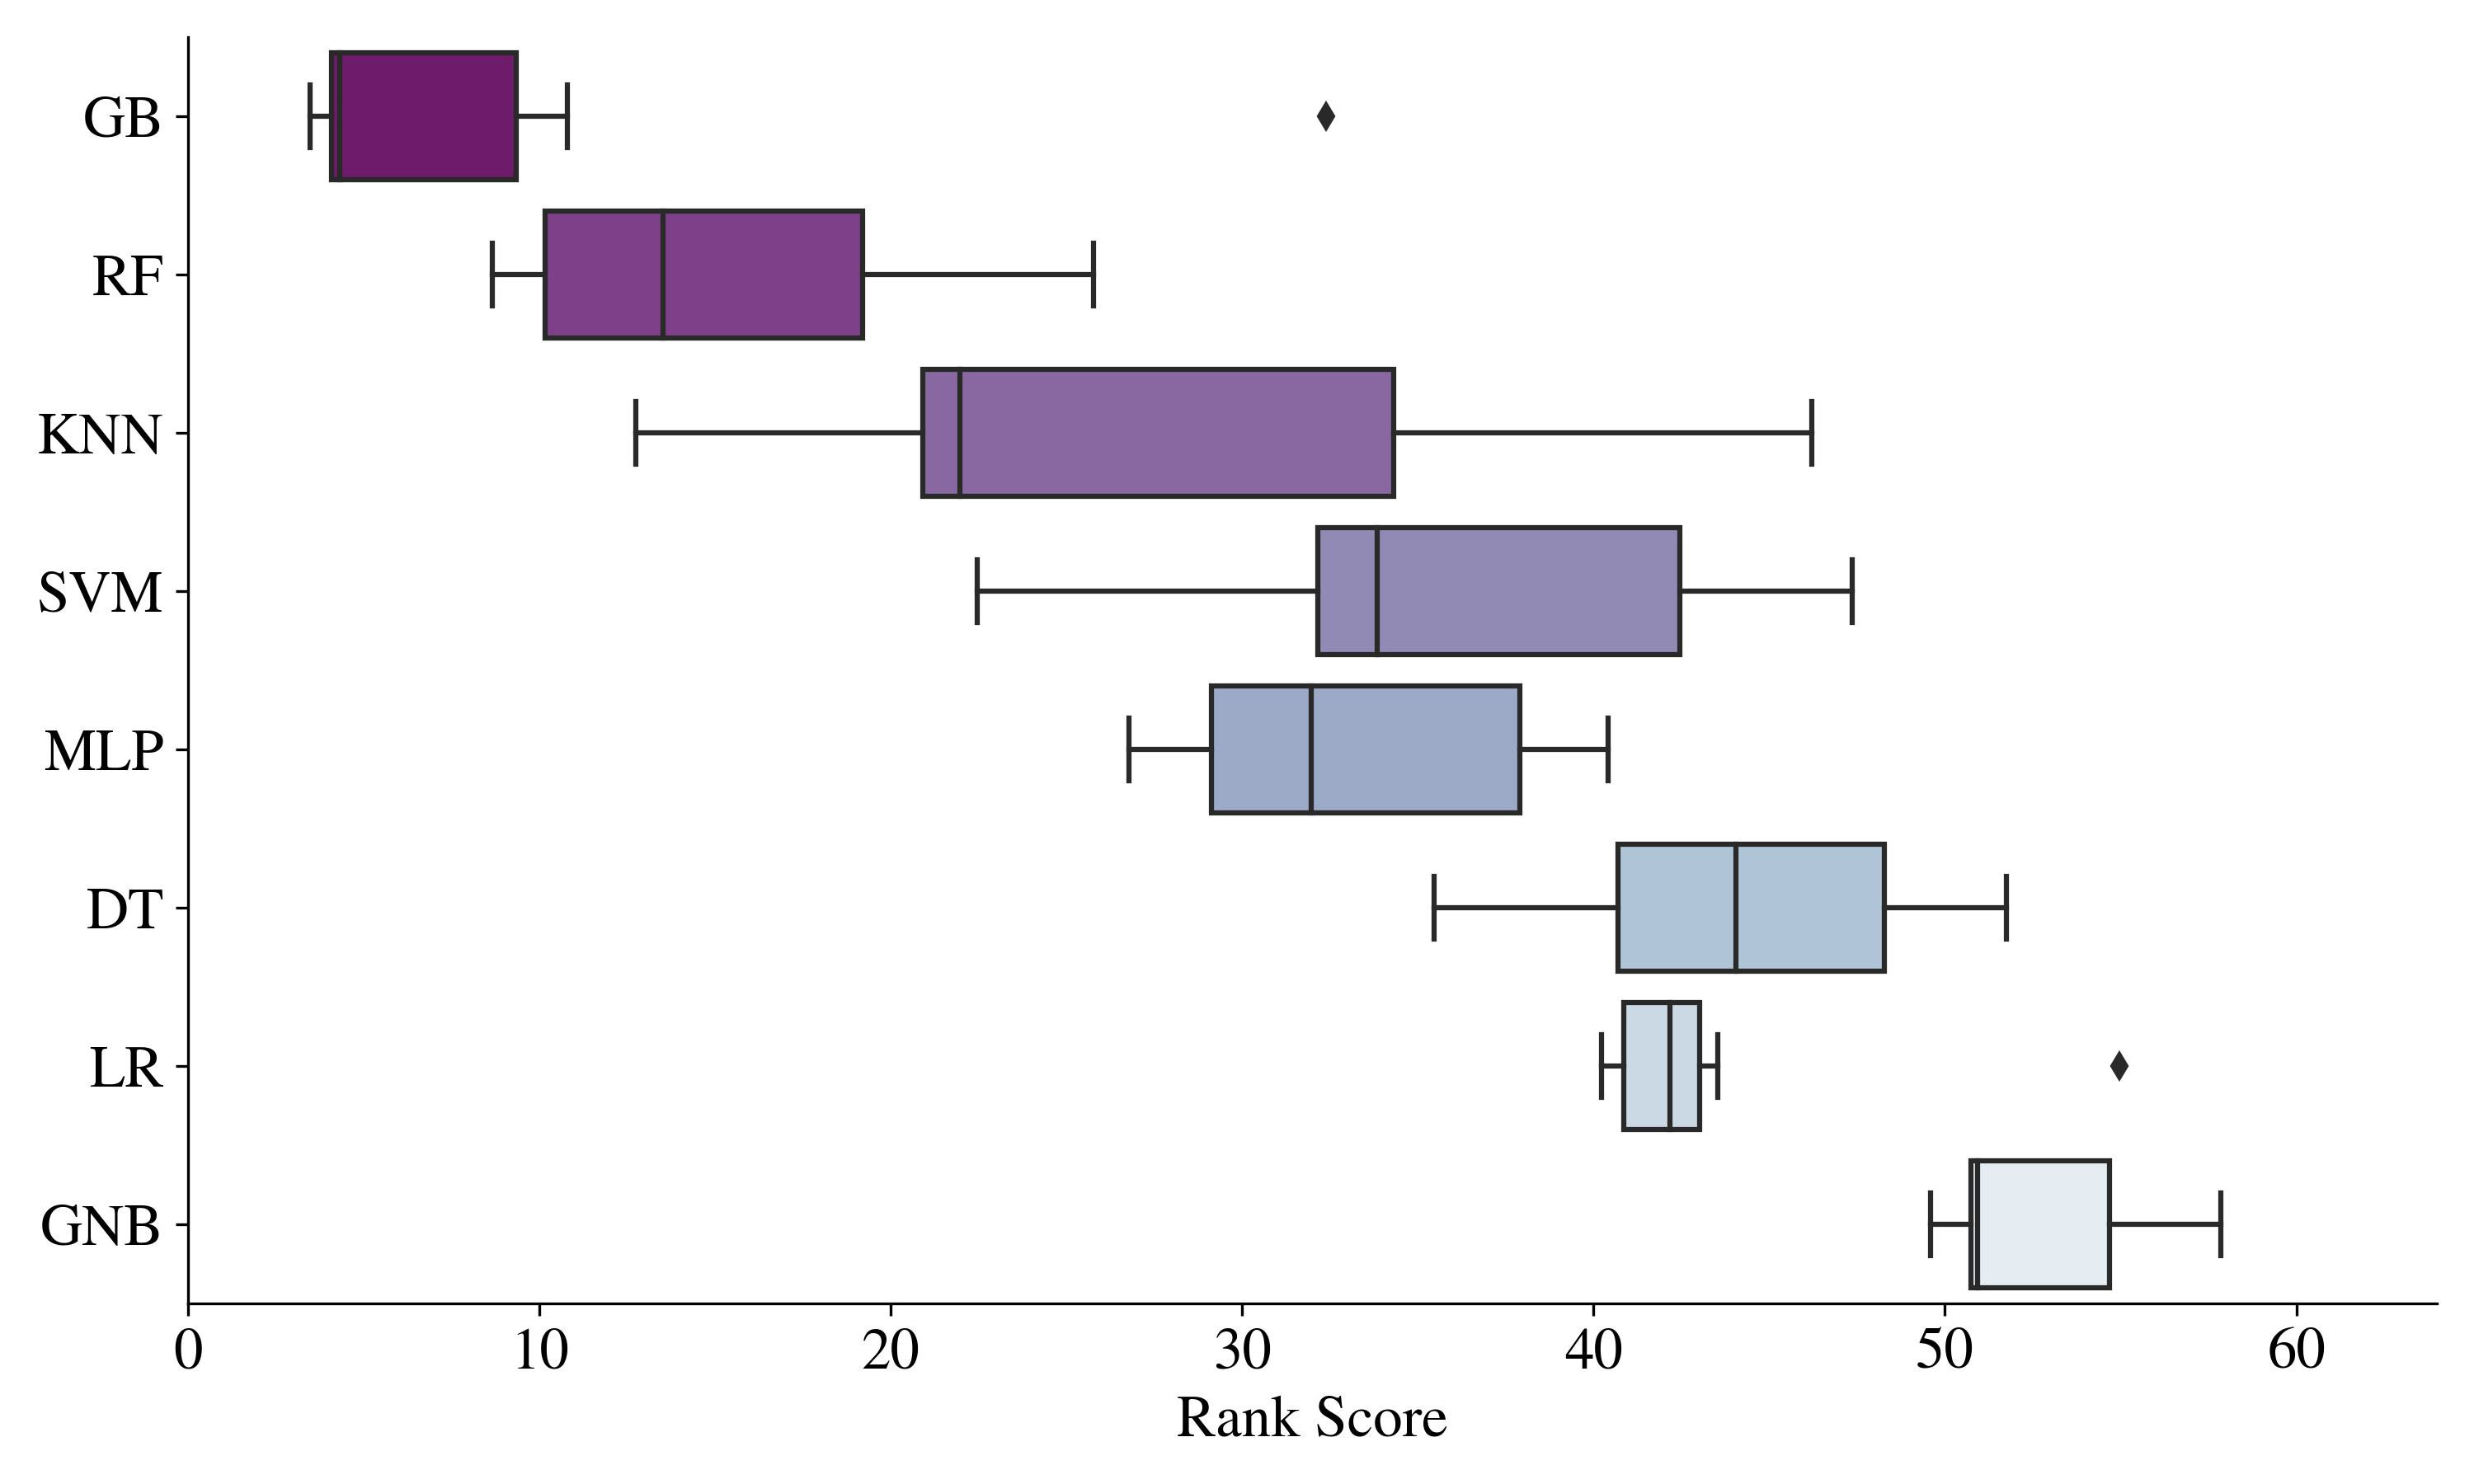
\includegraphics[width=140mm]{Figures/AVG_Rank_score_Distribution.jpg}
    \centering{\begin{source}Author's results in Python\end{source}}\vspace{-1em}
\end{figure}

As expected, also, the black--box models are ranked higher than the white--box models according to the rank score as shown in \autoref{fig:avgrankdistbbwb}. This is evident also from \autoref{tab:modelsectab} where the black--box models, namely Gradient Boosting and Random Forest, dominated amongst the first 10 ranked models.
\begin{figure}[H]
    \centering
    \caption{Rank Score distribution (Black--box/White--box dimension)}\vspace{0.5em}
    \label{fig:avgrankdistbbwb}\
    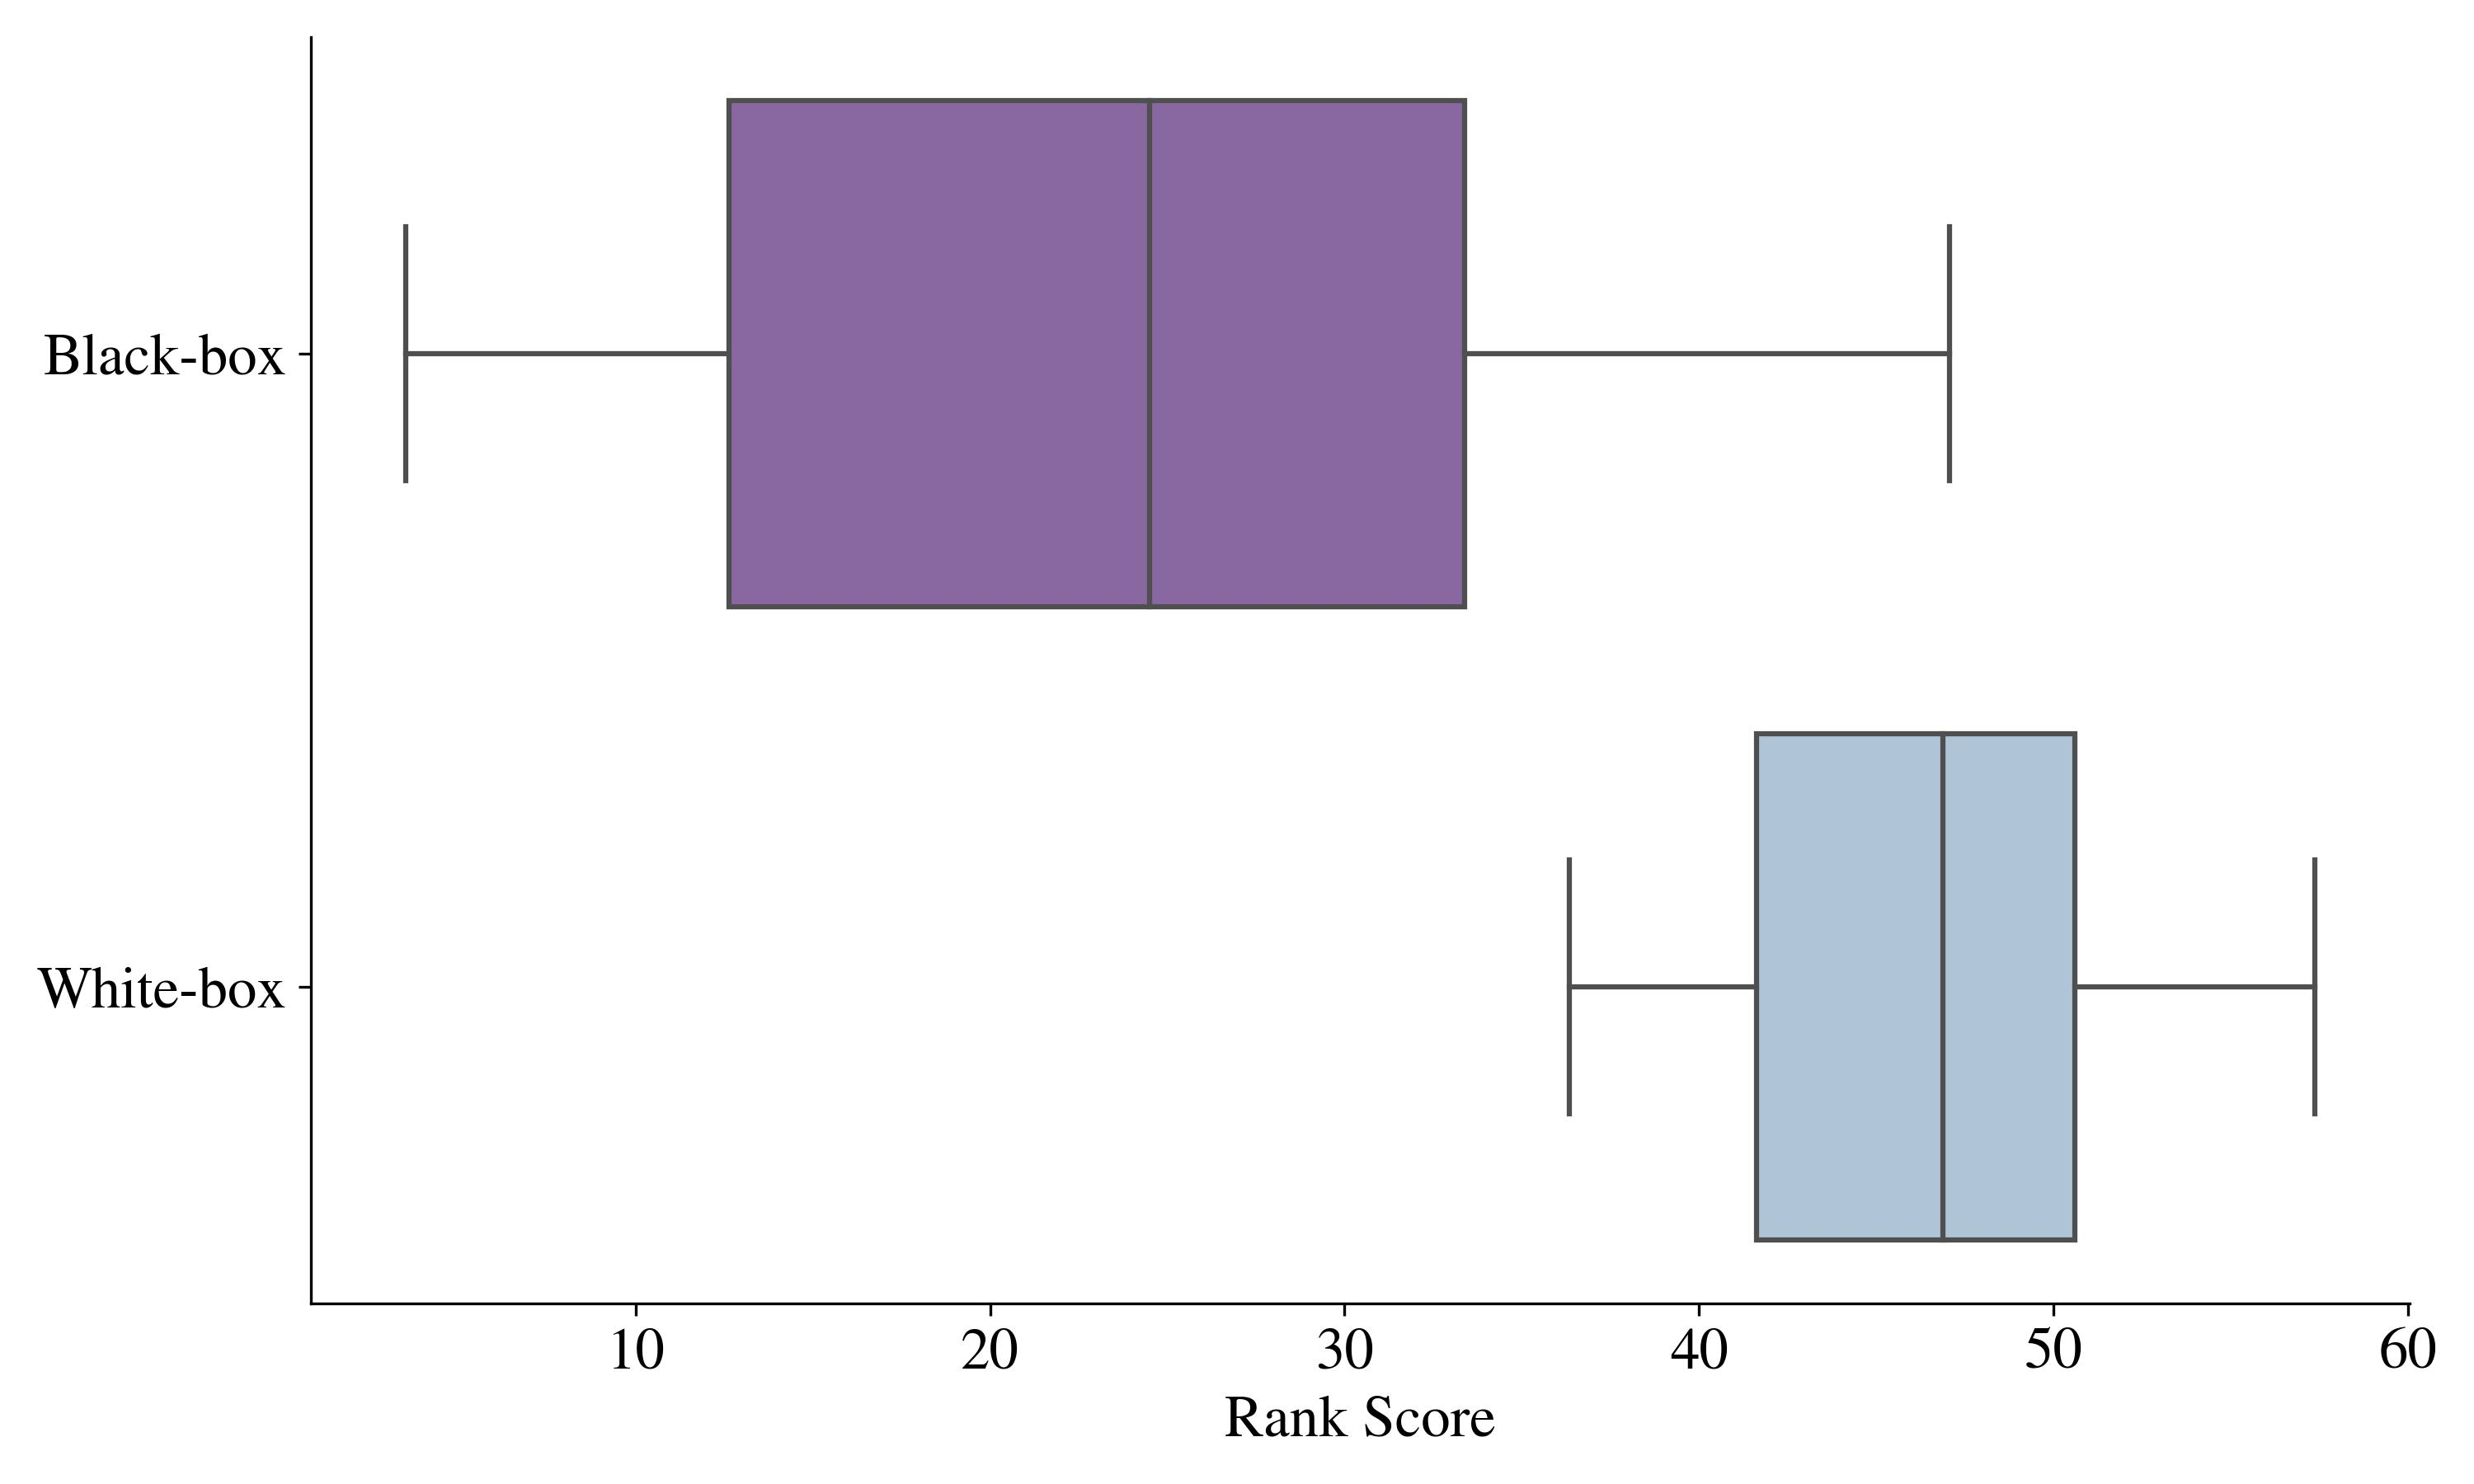
\includegraphics[width=140mm]{Figures/AVG_Rank_score_Distribution_BB_WB.jpg}
    \centering{\begin{source}Author's results in Python\end{source}}\vspace{-1em}
\end{figure}


The optimal threshold distribution for each base model is presented in \autoref{fig:thresdist}. We can observe an outlier in KNN having a threshold value of 1, which explains the F1 score outlier found previously in \autoref{fig:f1dist}.
\begin{figure}[H]
\centering
\caption{Threshold distribution}\vspace{0.5em}
\label{fig:thresdist}\
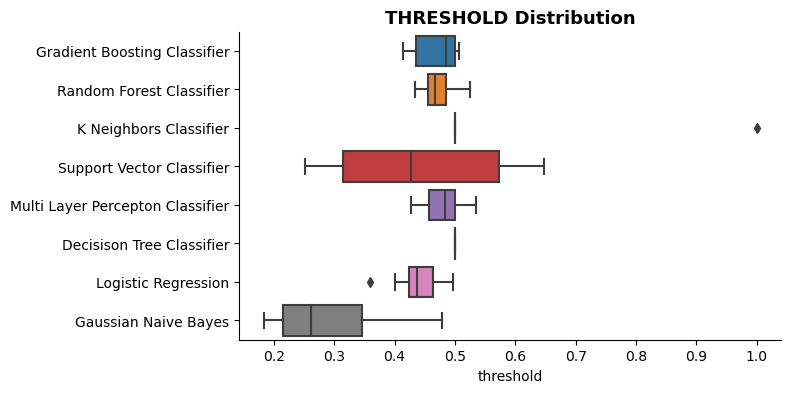
\includegraphics[width=140mm]{Figures/Threshold_Distribution.jpg}
\centering{\begin{source}Author's results in Python\end{source}}\vspace{-1em}
\end{figure}

In order to obtain a better insight into the distribution of optimal thresholds, the outlier in KNN is excluded, resulting in the threshold distribution depicted in \autoref{fig:thresdistclean}. The optimal threshold values are mostly distributed below 0.5, indicating that the models are generally more conservative. The most conservative model is Gaussian Naive Bayes, which has a median threshold value around 0.25.
\begin{figure}[H]
\centering
\caption{Threshold distribution - without outliers}\vspace{0.5em}
\label{fig:thresdistclean}\
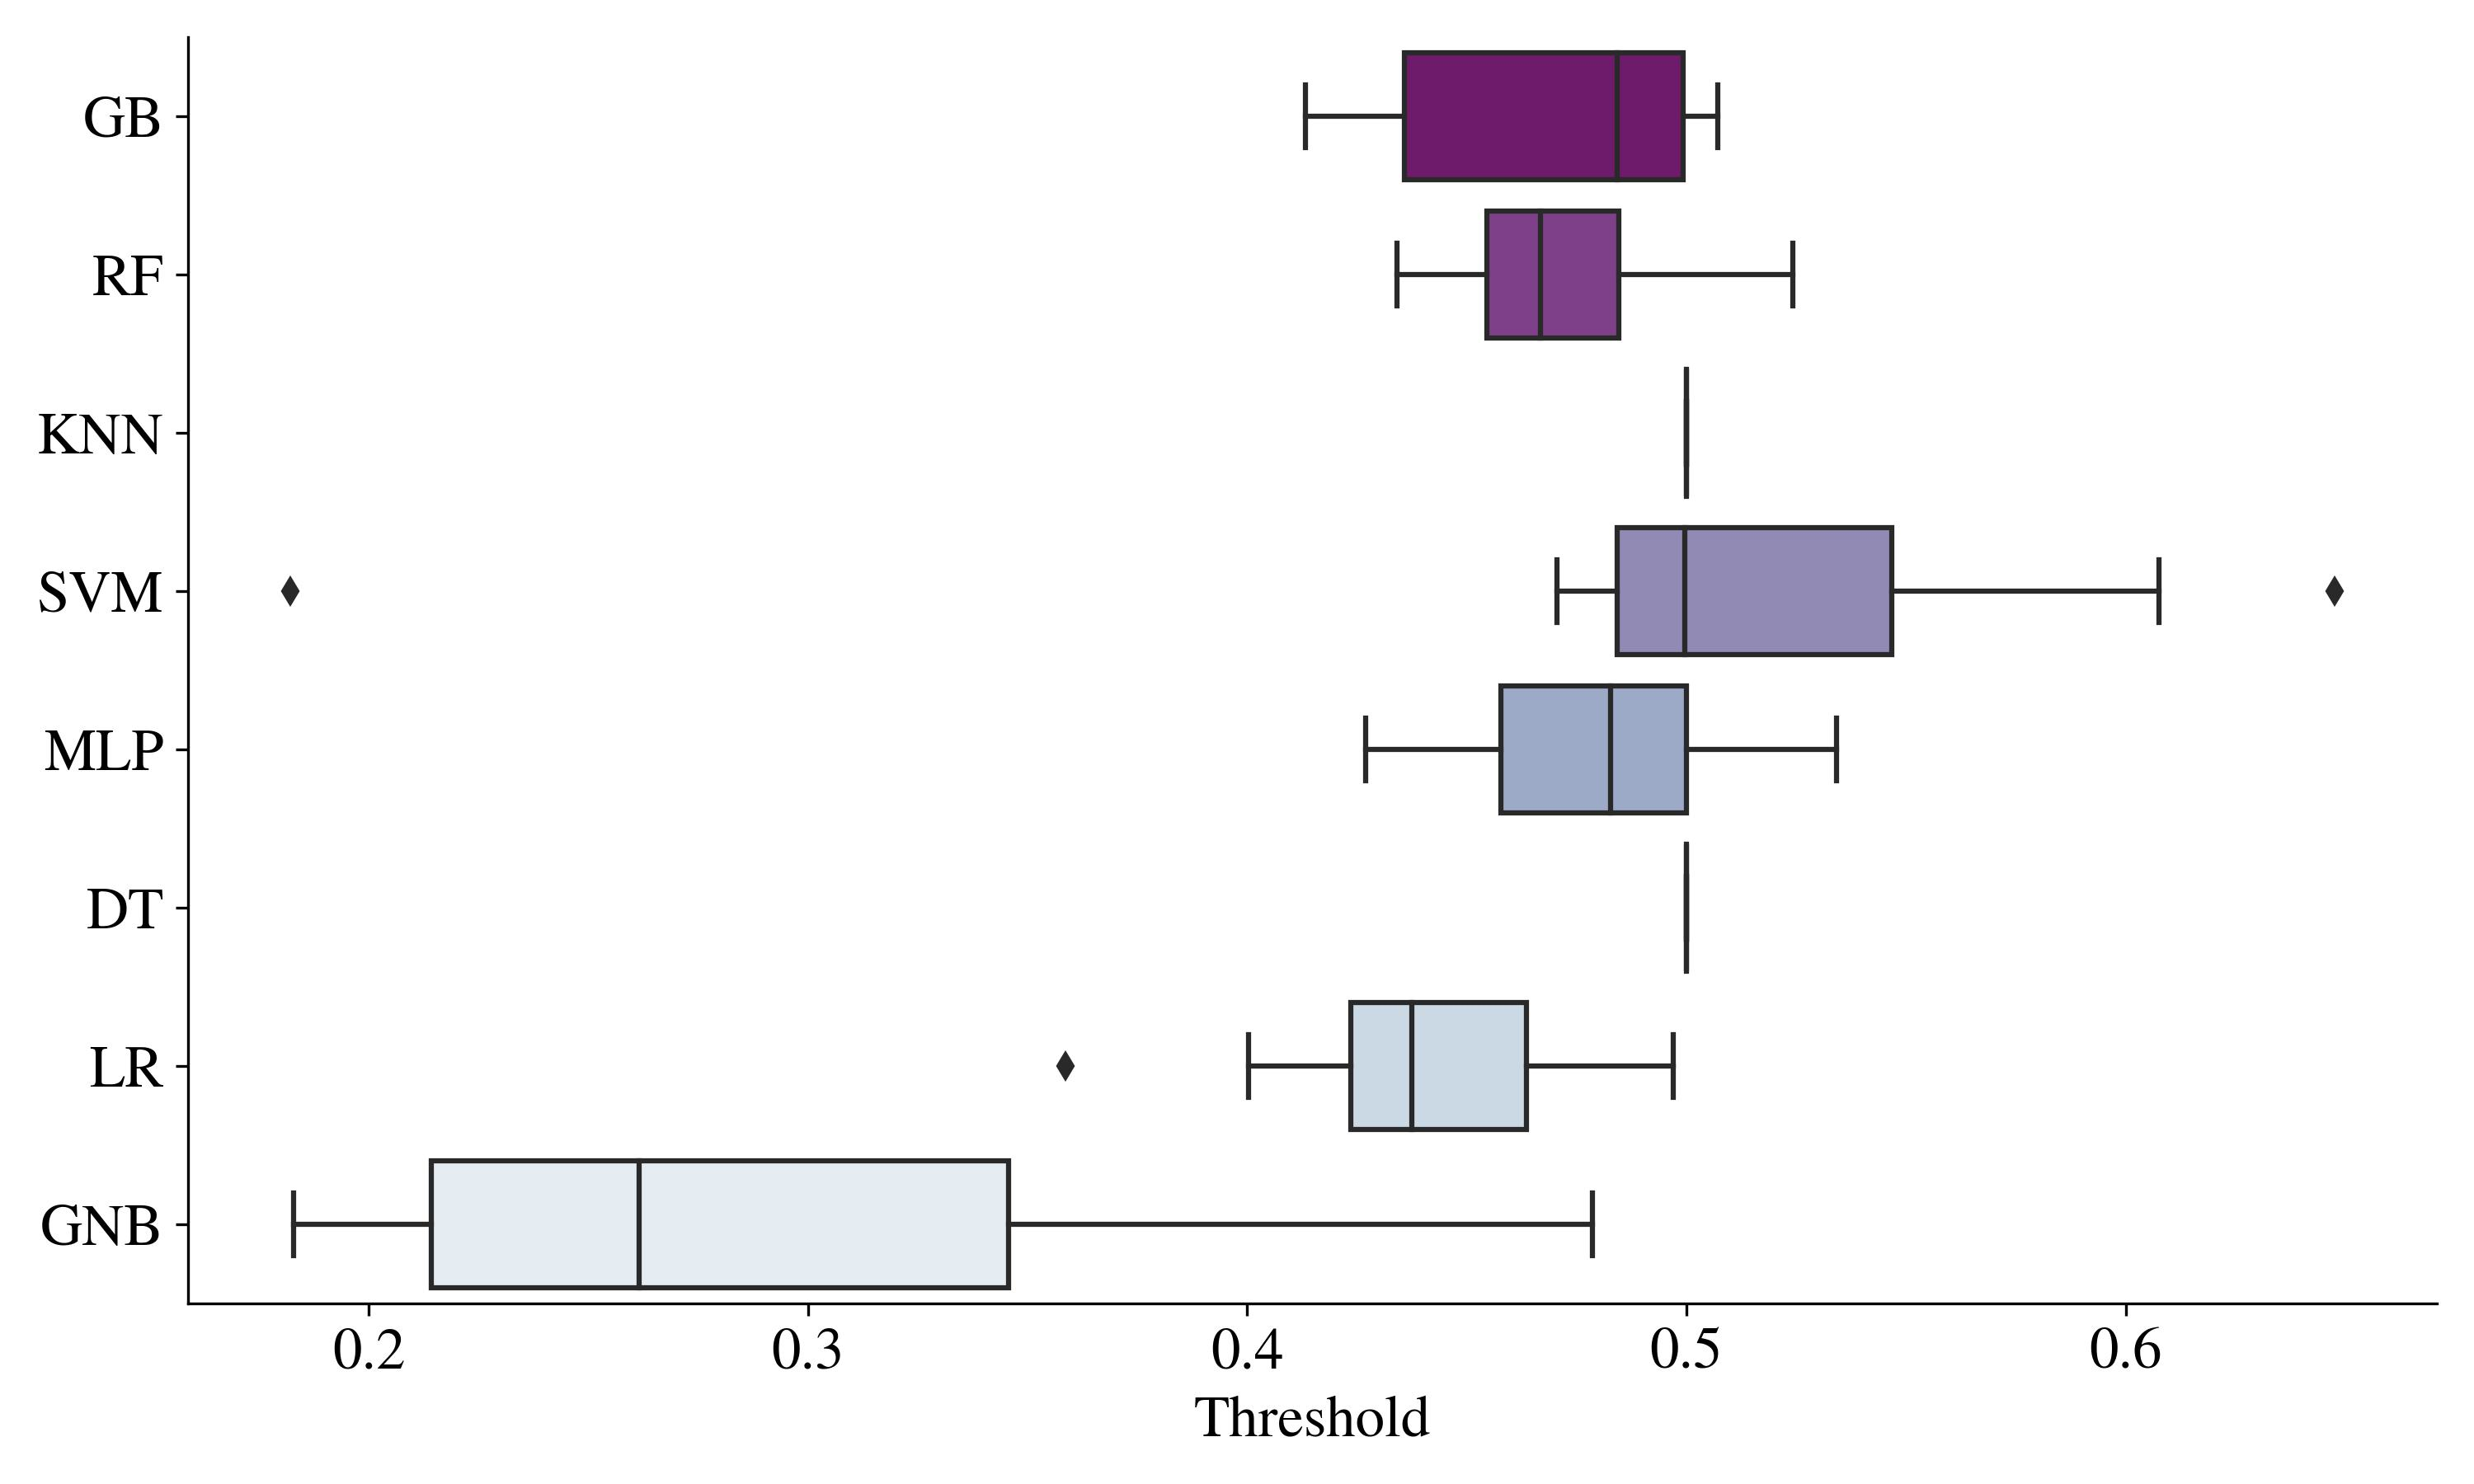
\includegraphics[width=140mm]{Figures/Threshold_wo_outliers_Distribution.jpg}
\centering{\begin{source}Author's results in Python\end{source}}\vspace{-1em}
\end{figure}




Upon examining the execution time of each model, it can be observed that the transparent and non-complex models such as Logistic Regression, Gaussian Naive Bayes, or even Decision Tree, which take around only 1 minute to optimize themselves, also perform poorly, as already inspected in \autoref{fig:f1distclean}.
Conversely, the most time-consuming models are undoubtedly the Neural Network models, which take around 30 minutes to optimize themselves. Other time-consuming models include Gradient Boosting and Support Vector Machine, which take around 13 and 11 minutes to optimize themselves, respectively.
This finding suggests that longer execution time does not necessarily lead to better performance, as the Neural Network models are significantly outperformed by several other models.
\begin{figure}[H]
\centering
\caption{Execution time distribution}\vspace{0.5em}
\label{fig:timedist}\
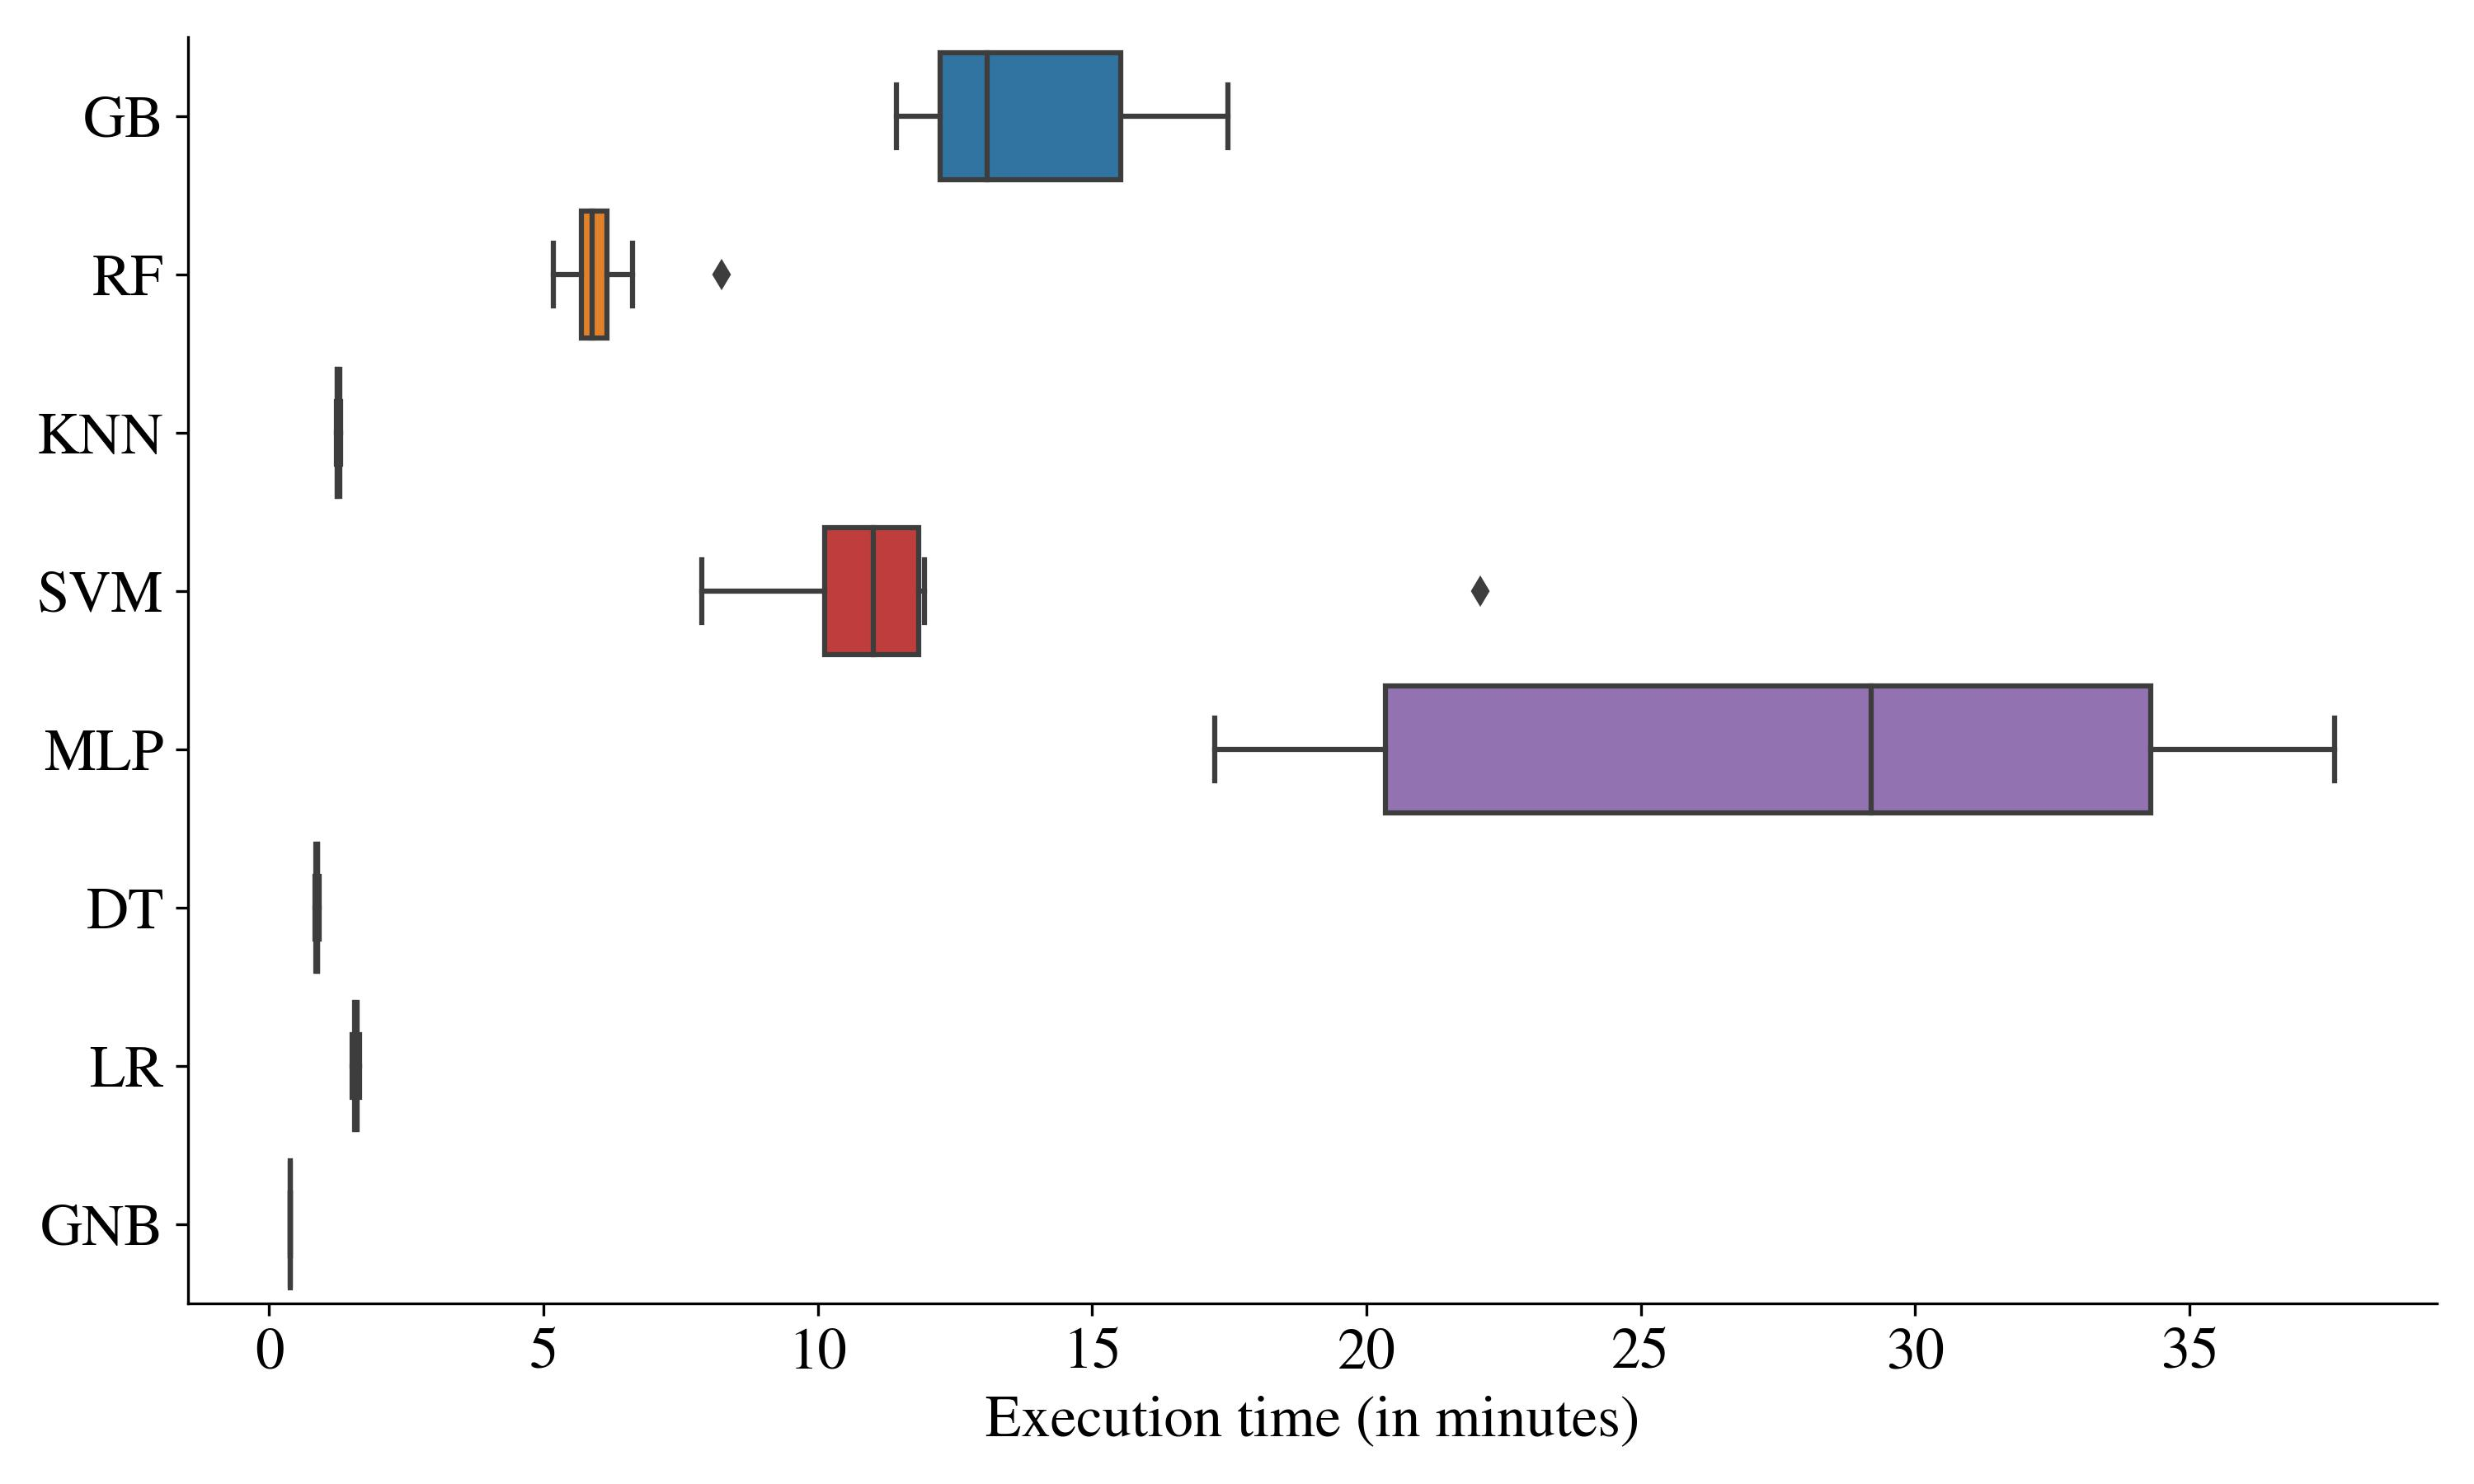
\includegraphics[width=140mm]{Figures/EXECUTION_TIME_Distribution.jpg}
\centering{\begin{source}Author's results in Python\end{source}}\vspace{-1em}
\end{figure}
We can inspect the execution from another perspective as shown in \autoref{fig:timedistbbwb}.
It can be observed that black--box models take a significant amount of time ot opimize than the white--box models which is given due to the complexity of the black--box models.
\begin{figure}[H]
    \centering
    \caption{Execution time distribution (Black--box/White--box dimension)}\vspace{0.5em}
    \label{fig:timedistbbwb}\
    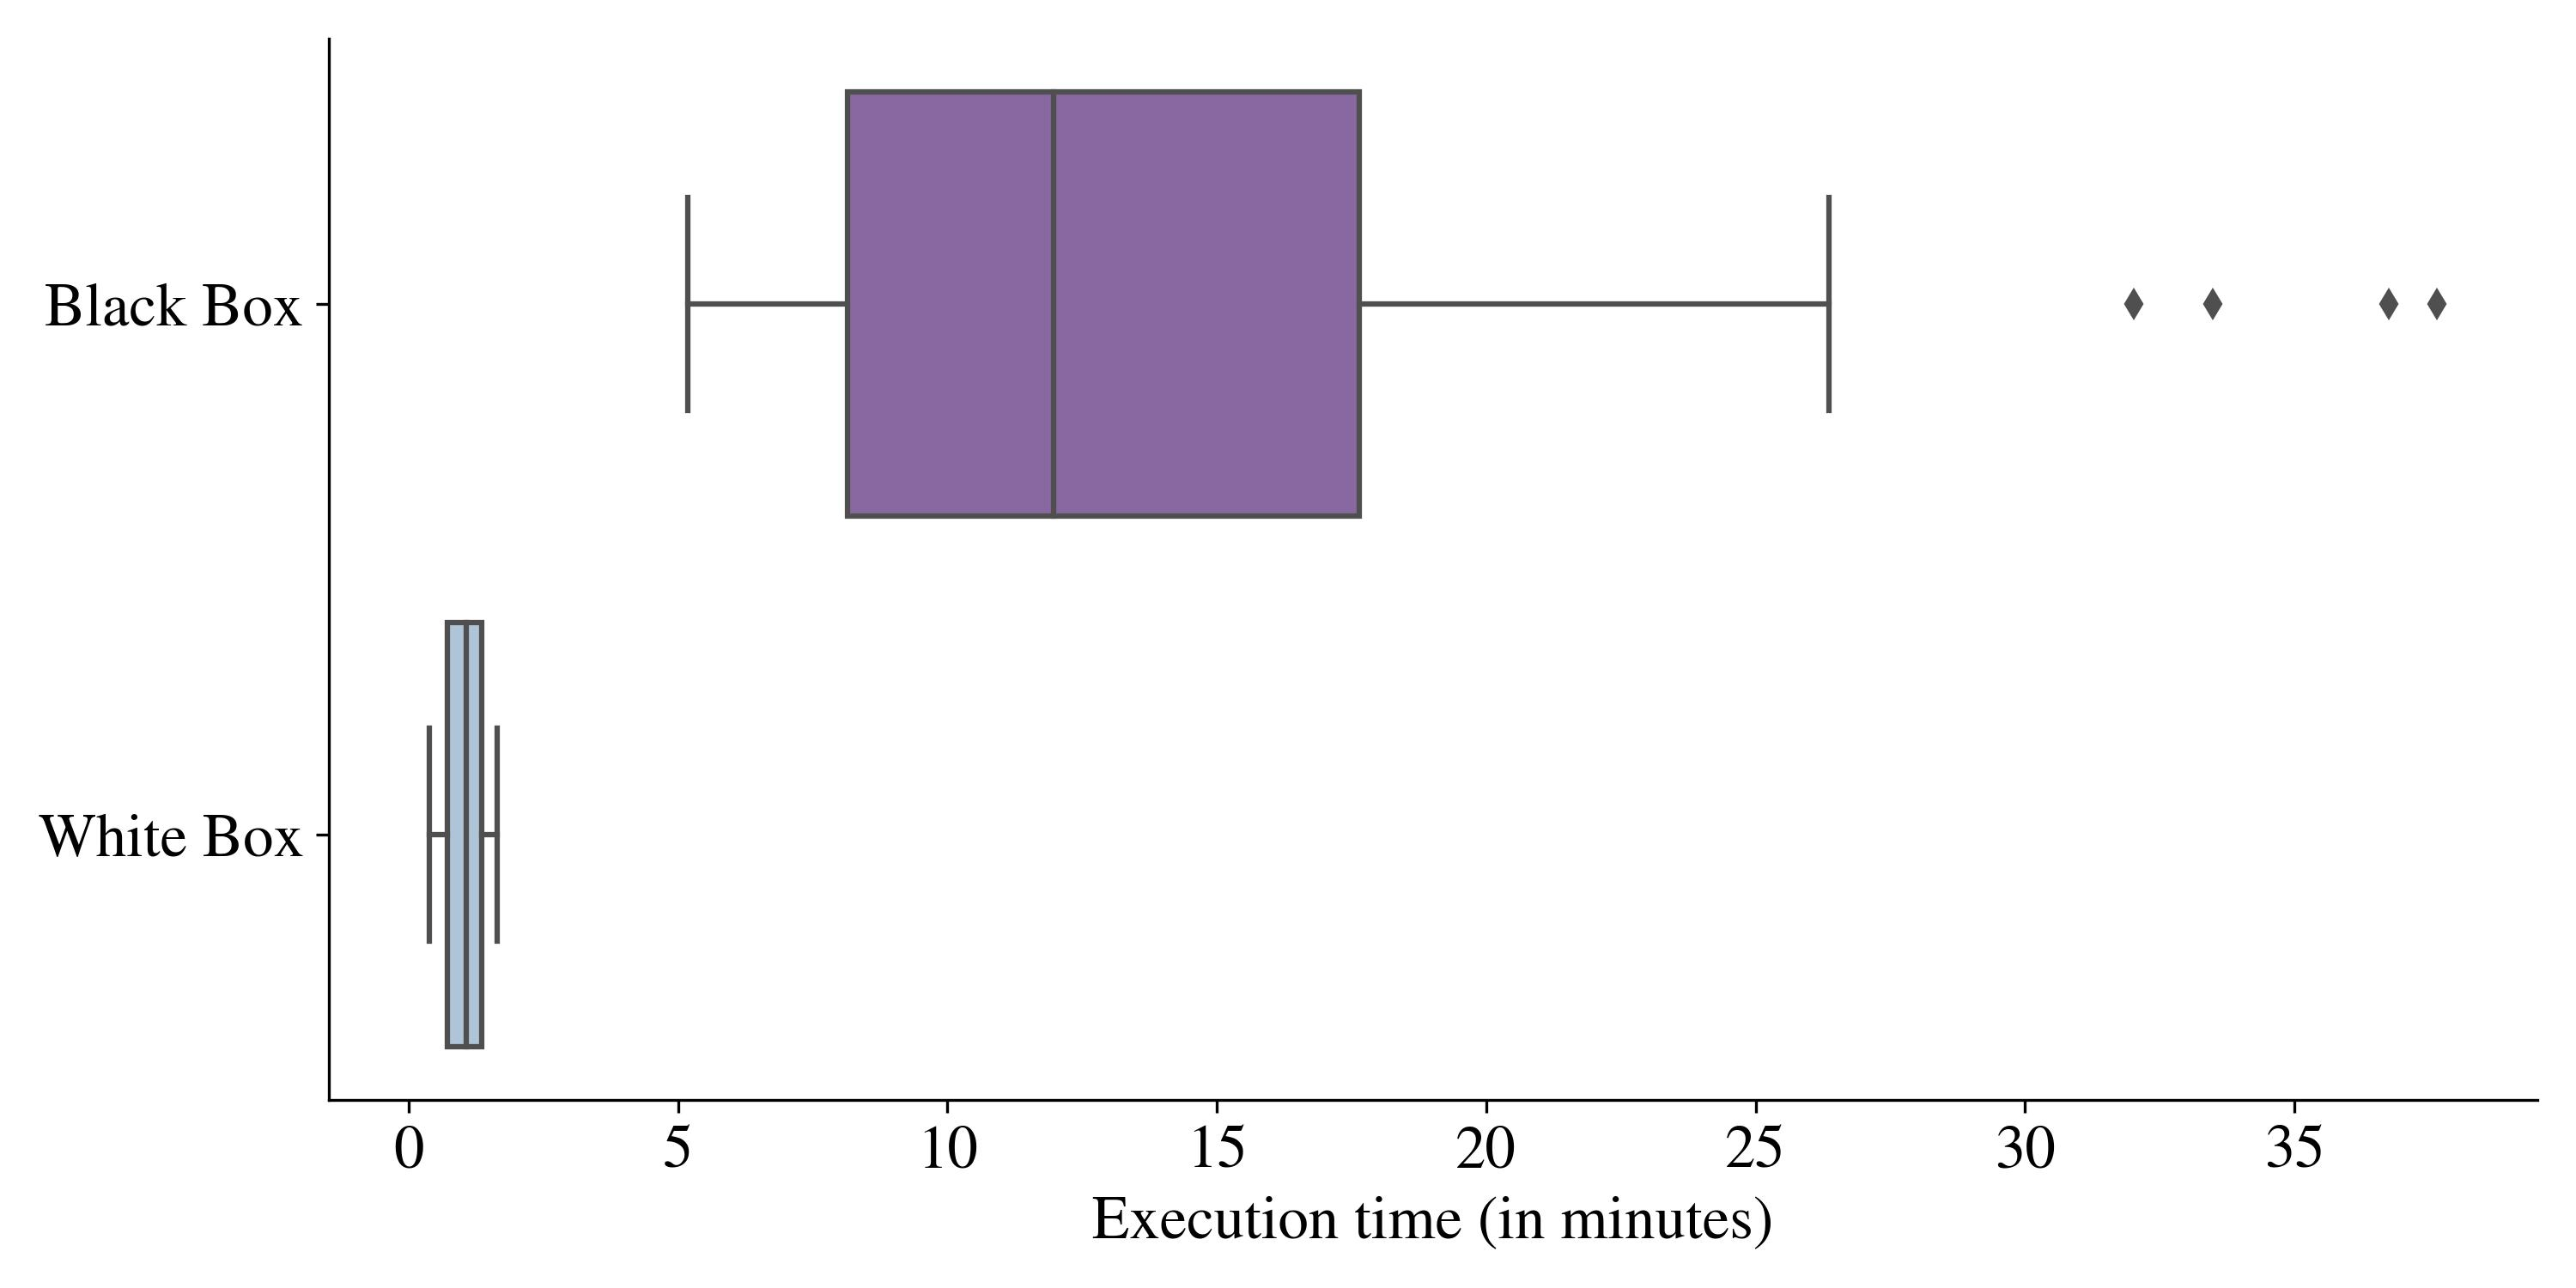
\includegraphics[width=140mm]{Figures/EXECUTION_TIME_Distribution_WB_BB.jpg}
    \centering{\begin{source}Author's results in Python\end{source}}\vspace{-1em}
\end{figure}


The execution time and the F1 score are inspected together using a scatterplot, as shown in \autoref{fig:scattertime}. 
A cluster of non-complex and transparent models, such as Logistic Regression, Gaussian Naive Bayes, Decision Tree, and KNN, can be observed around the vertical line near 0 execution time. These models are quick to optimize, but their F1 scores are generally low, except for KNN.
Further, their variance in execution time is quite low, regardless of the feature subset they are optimized on.
On the other hand, the Neural Network models always perform poorly, regardless of the length of the execution time. Furthermore, the variance of the F1 scores is quite low for these models, indicating that the execution time does not have a significant impact on the F1 score in the case of Neural Networks.

\begin{figure}[H]
\centering
\caption{Execution time vs. F1 Scatterplot - without outlier}\vspace{0.5em}
\label{fig:scattertime}\
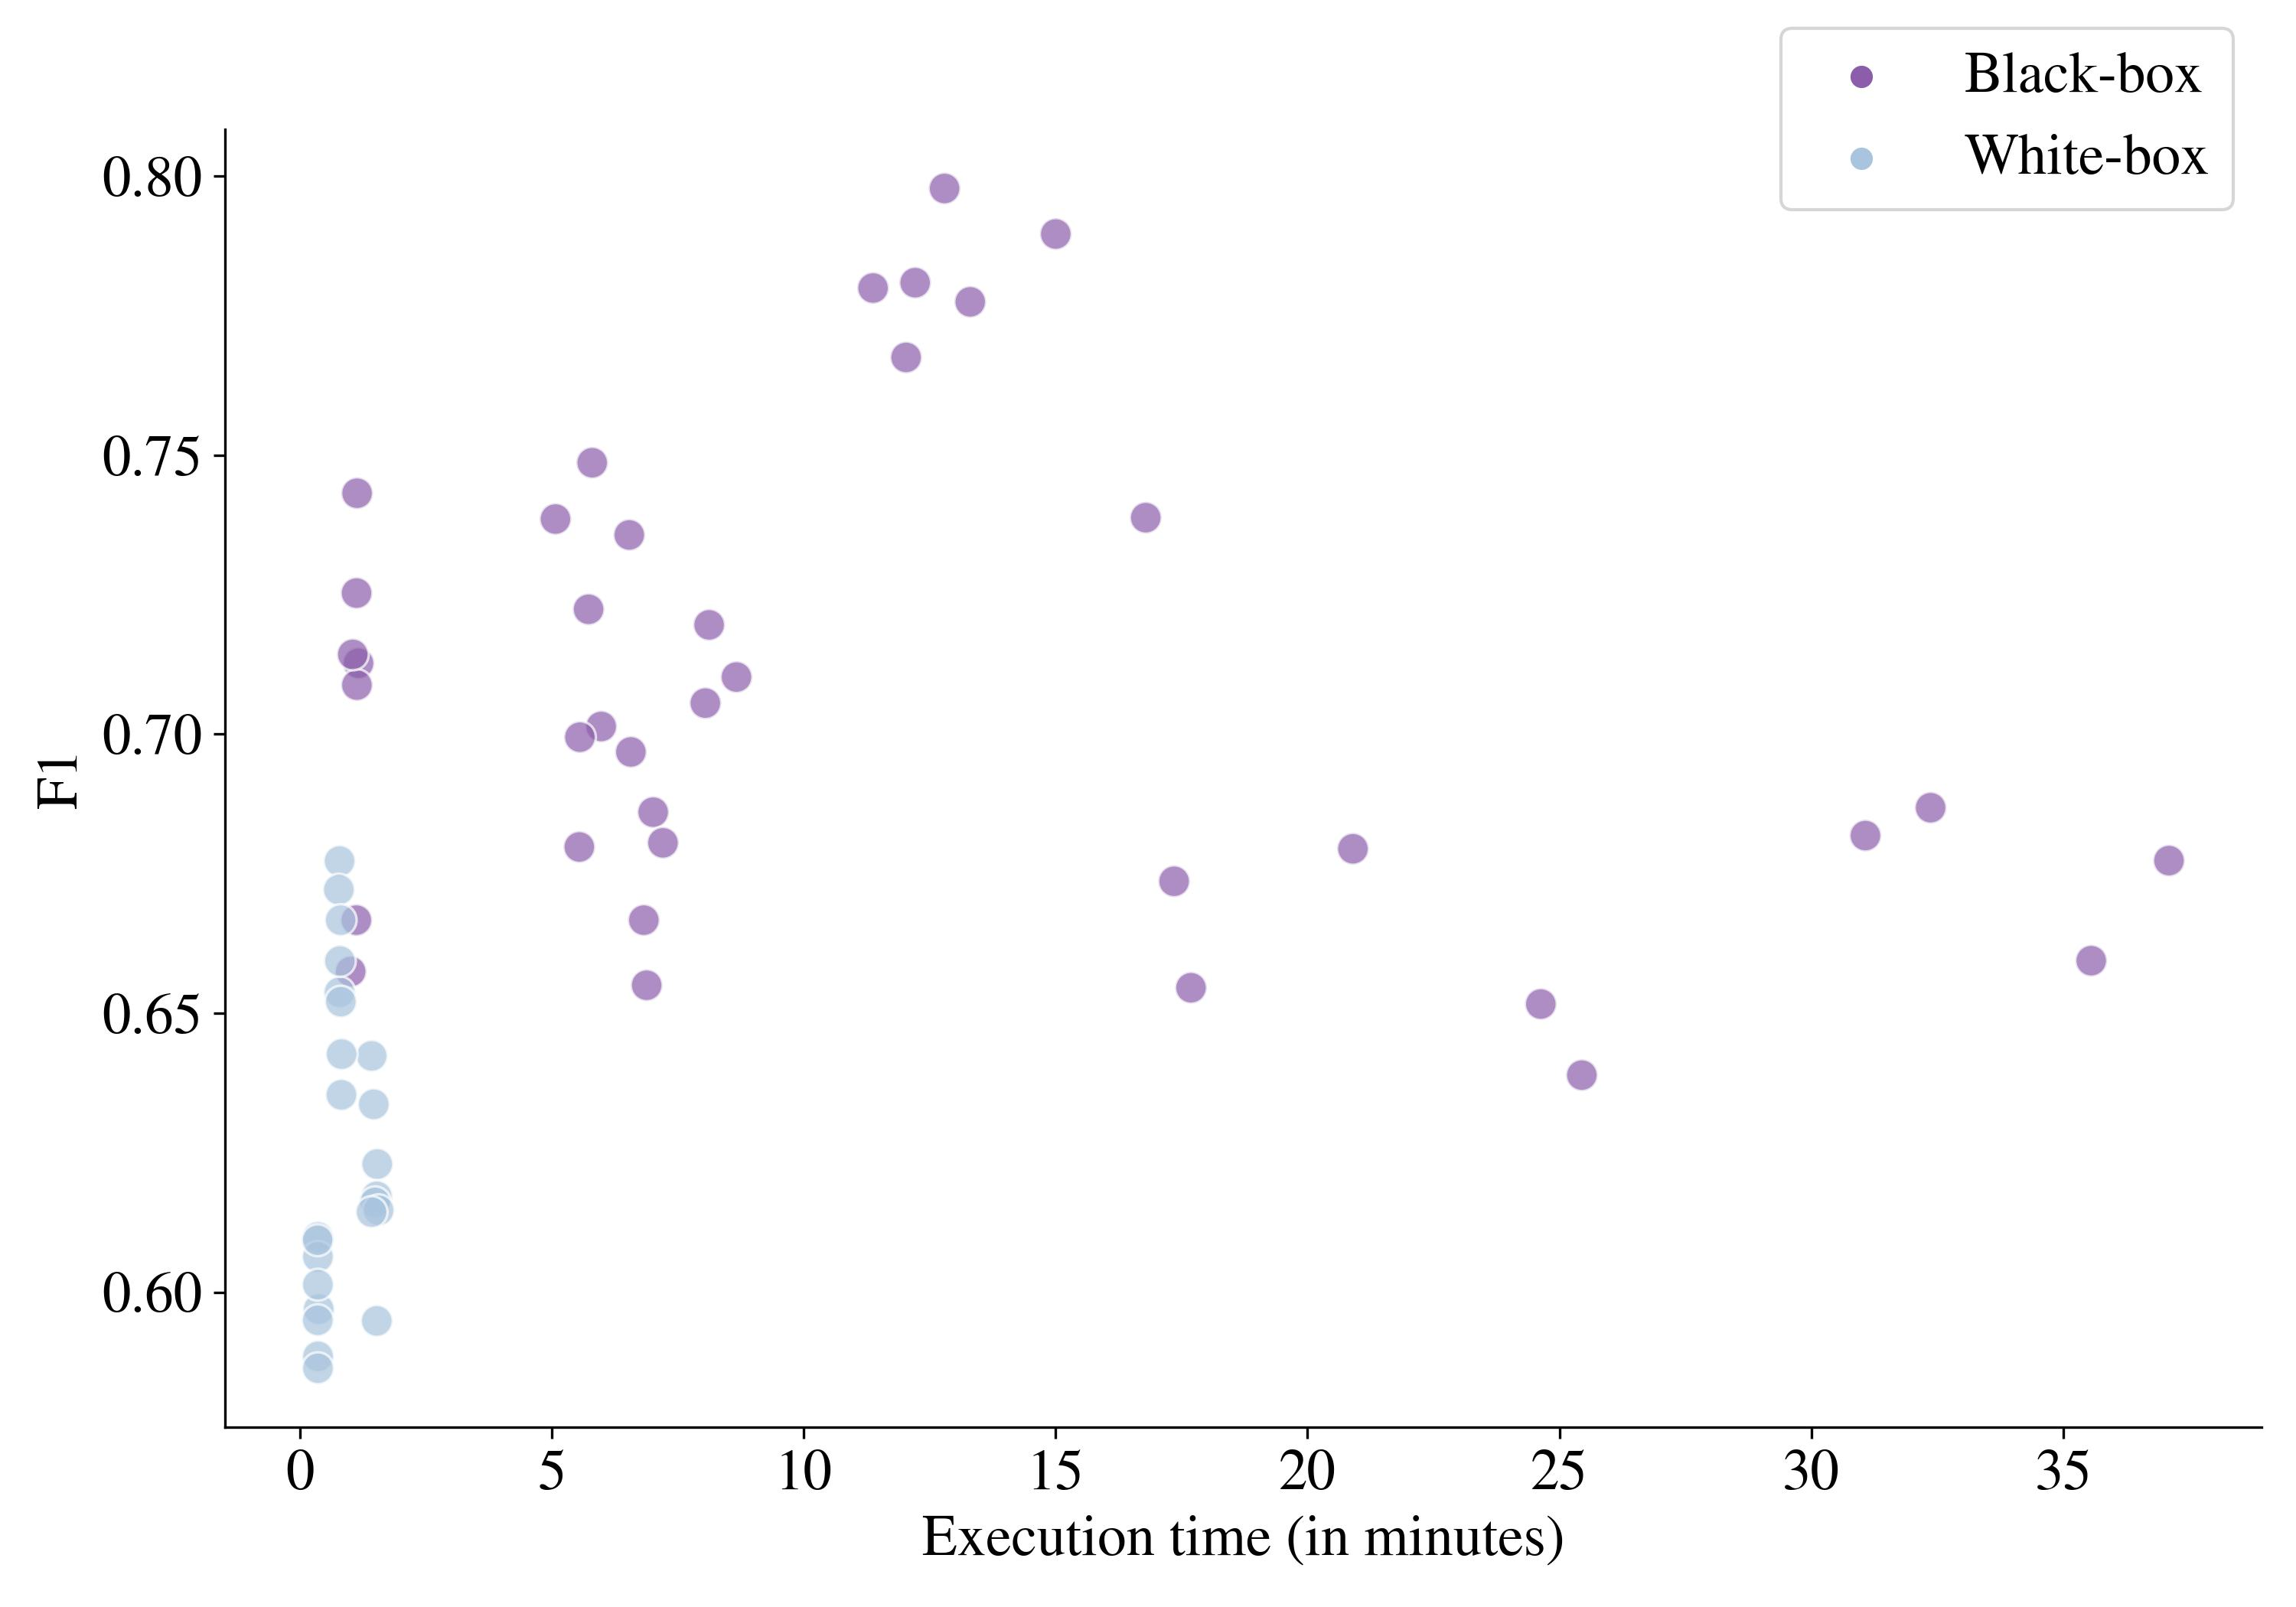
\includegraphics[width=140mm]{Figures/Scatterplot_execution_time_F1_wo_outliers.jpg}
\centering{\begin{source}Author's results in Python\end{source}}\vspace{-1em}
\end{figure}
Such separation of of the black--box and white--box models is more evident from \autoref{fig:scattertimebbwb} where the white--box models points are light blue-colored and the black--box models are purple-colored.
While the execution time of white--box models seems to be constant regardless the score, the points of black--box models are more dispersed across the execution time--F1 dimension.

\begin{figure}[H]
    \centering
    \caption{Execution time vs. F1 Scatterplot (Black--box/White--box dimension) - without outlier}\vspace{0.5em}
    \label{fig:scattertimebbwb}\
    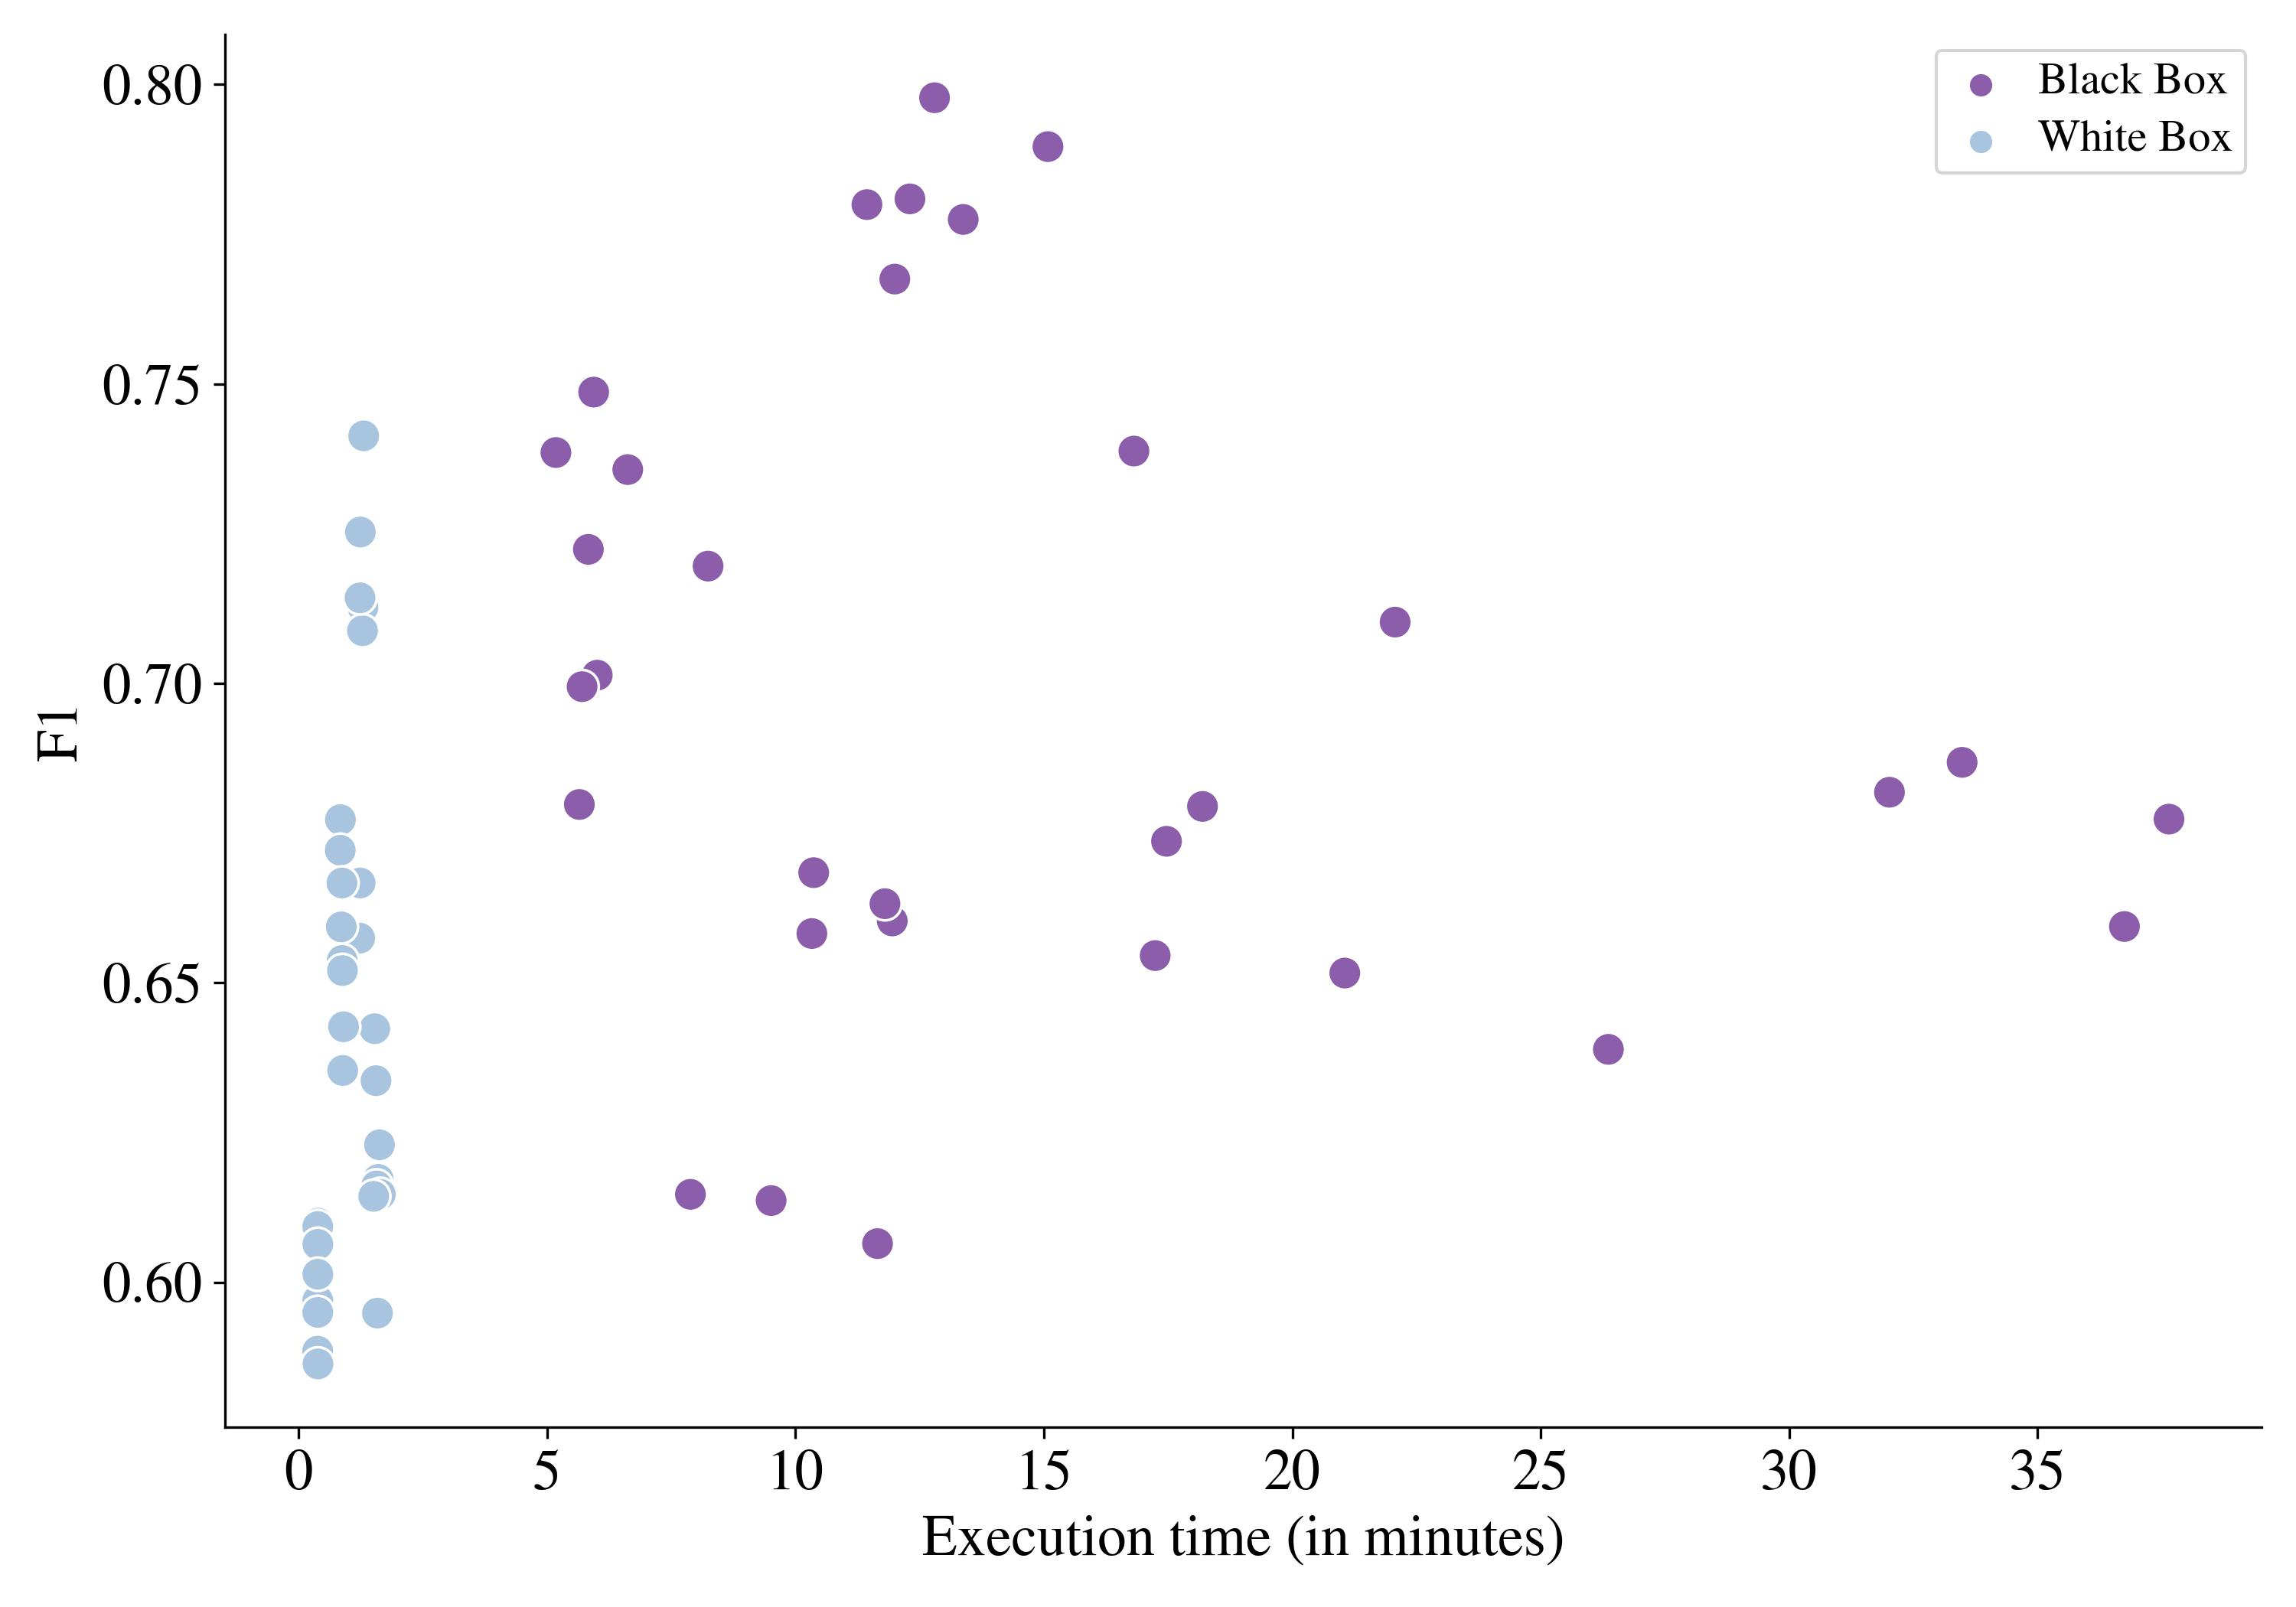
\includegraphics[width=140mm]{Figures/Scatterplot_execution_time_F1_wo_outliers_BB_WB.jpg}
    \centering{\begin{source}Author's results in Python\end{source}}\vspace{-1em}
\end{figure}


To summarize this subsection, the best and final model is the Gradient Boosting Classifier which was optimized on the subset of features selected by Multi-Layer Percepton - both the model information and its final hyperparameters' values are described in \autoref{tab:finalmodelinfo}. Such model is then used in the next modelling steps, including the recalibration, evaluation and deployment.
\begin{table}[H]
    \small
    \setlength{\tabcolsep}{8pt}
    \renewcommand{\arraystretch}{1.3}
    \centering
    \caption{Final Model Information}\label{tab:finalmodelinfo}
    \begin{tabular}{>{\raggedleft\arraybackslash}p{0.20\linewidth}|p{0.65\linewidth}}
    \toprule
    \midrule
    \textbf{Final Model} & Gradient Boosting \\
    \midrule
    \textbf{FS Model} & Multi--Layer Percepton \\
    \midrule
    \textbf{Final Features} &
    MORTDUE, VALUE, JOB, YOJ, DEROG, DELINQ, CLAGE, NINQ, CLNO, DEBTINC \\
    \midrule
    \textbf{Threshold} & 0.4955 \\
    \midrule
    \textbf{F1} & 0.7809 \\
    \midrule
    \textit{\# estimators} & 1,000 \\
    \midrule
    \textit{Criterion} & Friedman MSE \\
    \midrule
    \textit{Max depth} & 10 \\
    \midrule
    \textit{Max features} & 1 \\
    \midrule
    \textit{Loss} & Log loss \\
    \midrule
    \textit{Learning rate} & 0.0150 \\
    \midrule
    \bottomrule
    \end{tabular}
    \vspace{0.5em}
    
    \centering{\begin{source}Author's results in Python\end{source}}\vspace{-0.5em}
\end{table}

\newpage
\subsection{Model Recalibration}

In order to ensure that the final model performs well on unseen data, it is common practice to employ the recalibration approach, which involves retraining the model on both the training and validation sets.
By doing so, the sample size used for training is increased. As such, the retraining (or so called recalibration) model lead (or are expected to lead) to markedly improved model performance \citep{de2023predicting}.
The recalibrated model is then used to evaluate the performance of the final model on the test set, which is the ultimate measure of a model's performance.

In addition to recalibrating the final model, it is crucial to recalibrate the threshold value for assigning class labels based on predicted probabilities. The optimal threshold value can be determined using the training and validation sets. Such threshold is recalibrated based on the training and validation set.
In this thesis, the optimal threshold value is found to be \textbf{0.45109}, which is then used for evaluating the final model's performance on the test set.
By recalibrating the threshold value, the model's performance is further improved, resulting in more accurate predictions. After the recalibration process, we can observe that the model is more conservative as its optimal classification threshold has decreased. The impact on the model's performance is further assessed in \autoref{subsec:modelperformance}.

Moreover, the recalibration process helps to mitigate overfitting issues, which occur when the model is only trained on the training set.
By incorporating the validation set into the training process, the recalibrated model can better generalize to new data and improve its overall performance on the test set.
The inclusion of the validation set during the recalibration process does not cause any data leakage issues since this set was already used during model selection to evaluate each model's performance.
Therefore, using the validation data for recalibration is a sound practice that helps to ensure the reliability and accuracy of the final model.

\newpage
\section{Model Evaluation}
After recalibrating the model and threshold, the final step in evaluating the model's performance is to test it on previously unseen data, specifically the test set.
This evaluation is critical to determine whether the model can generalize well to new data beyond the training, feature selection, and model selection phases.
During the evaluation, the recalibrated classification threshold of 0.45109, determined in the model recalibration process, is also used.
\subsection{Model Performance Assessment}
\label{subsec:modelperformance}



In \autoref{fig:confmat}, the confusion matrix for the final model, based on the test set and using the recalibrated threshold, is presented. The matrix shows that the model is generalizing well, having correctly predicted 145 defaults and misclassified only 33 defaults and further, correctly predicted 683 non--defaults and misclassified only 33 non--defaults. Such a result indicates that the model is a good fit for the data and can provide useful predictions for the problem at hand.

\begin{figure}[H]
\centering
\caption{Confusion Matrix}\vspace{0.5em}
\label{fig:confmat}\
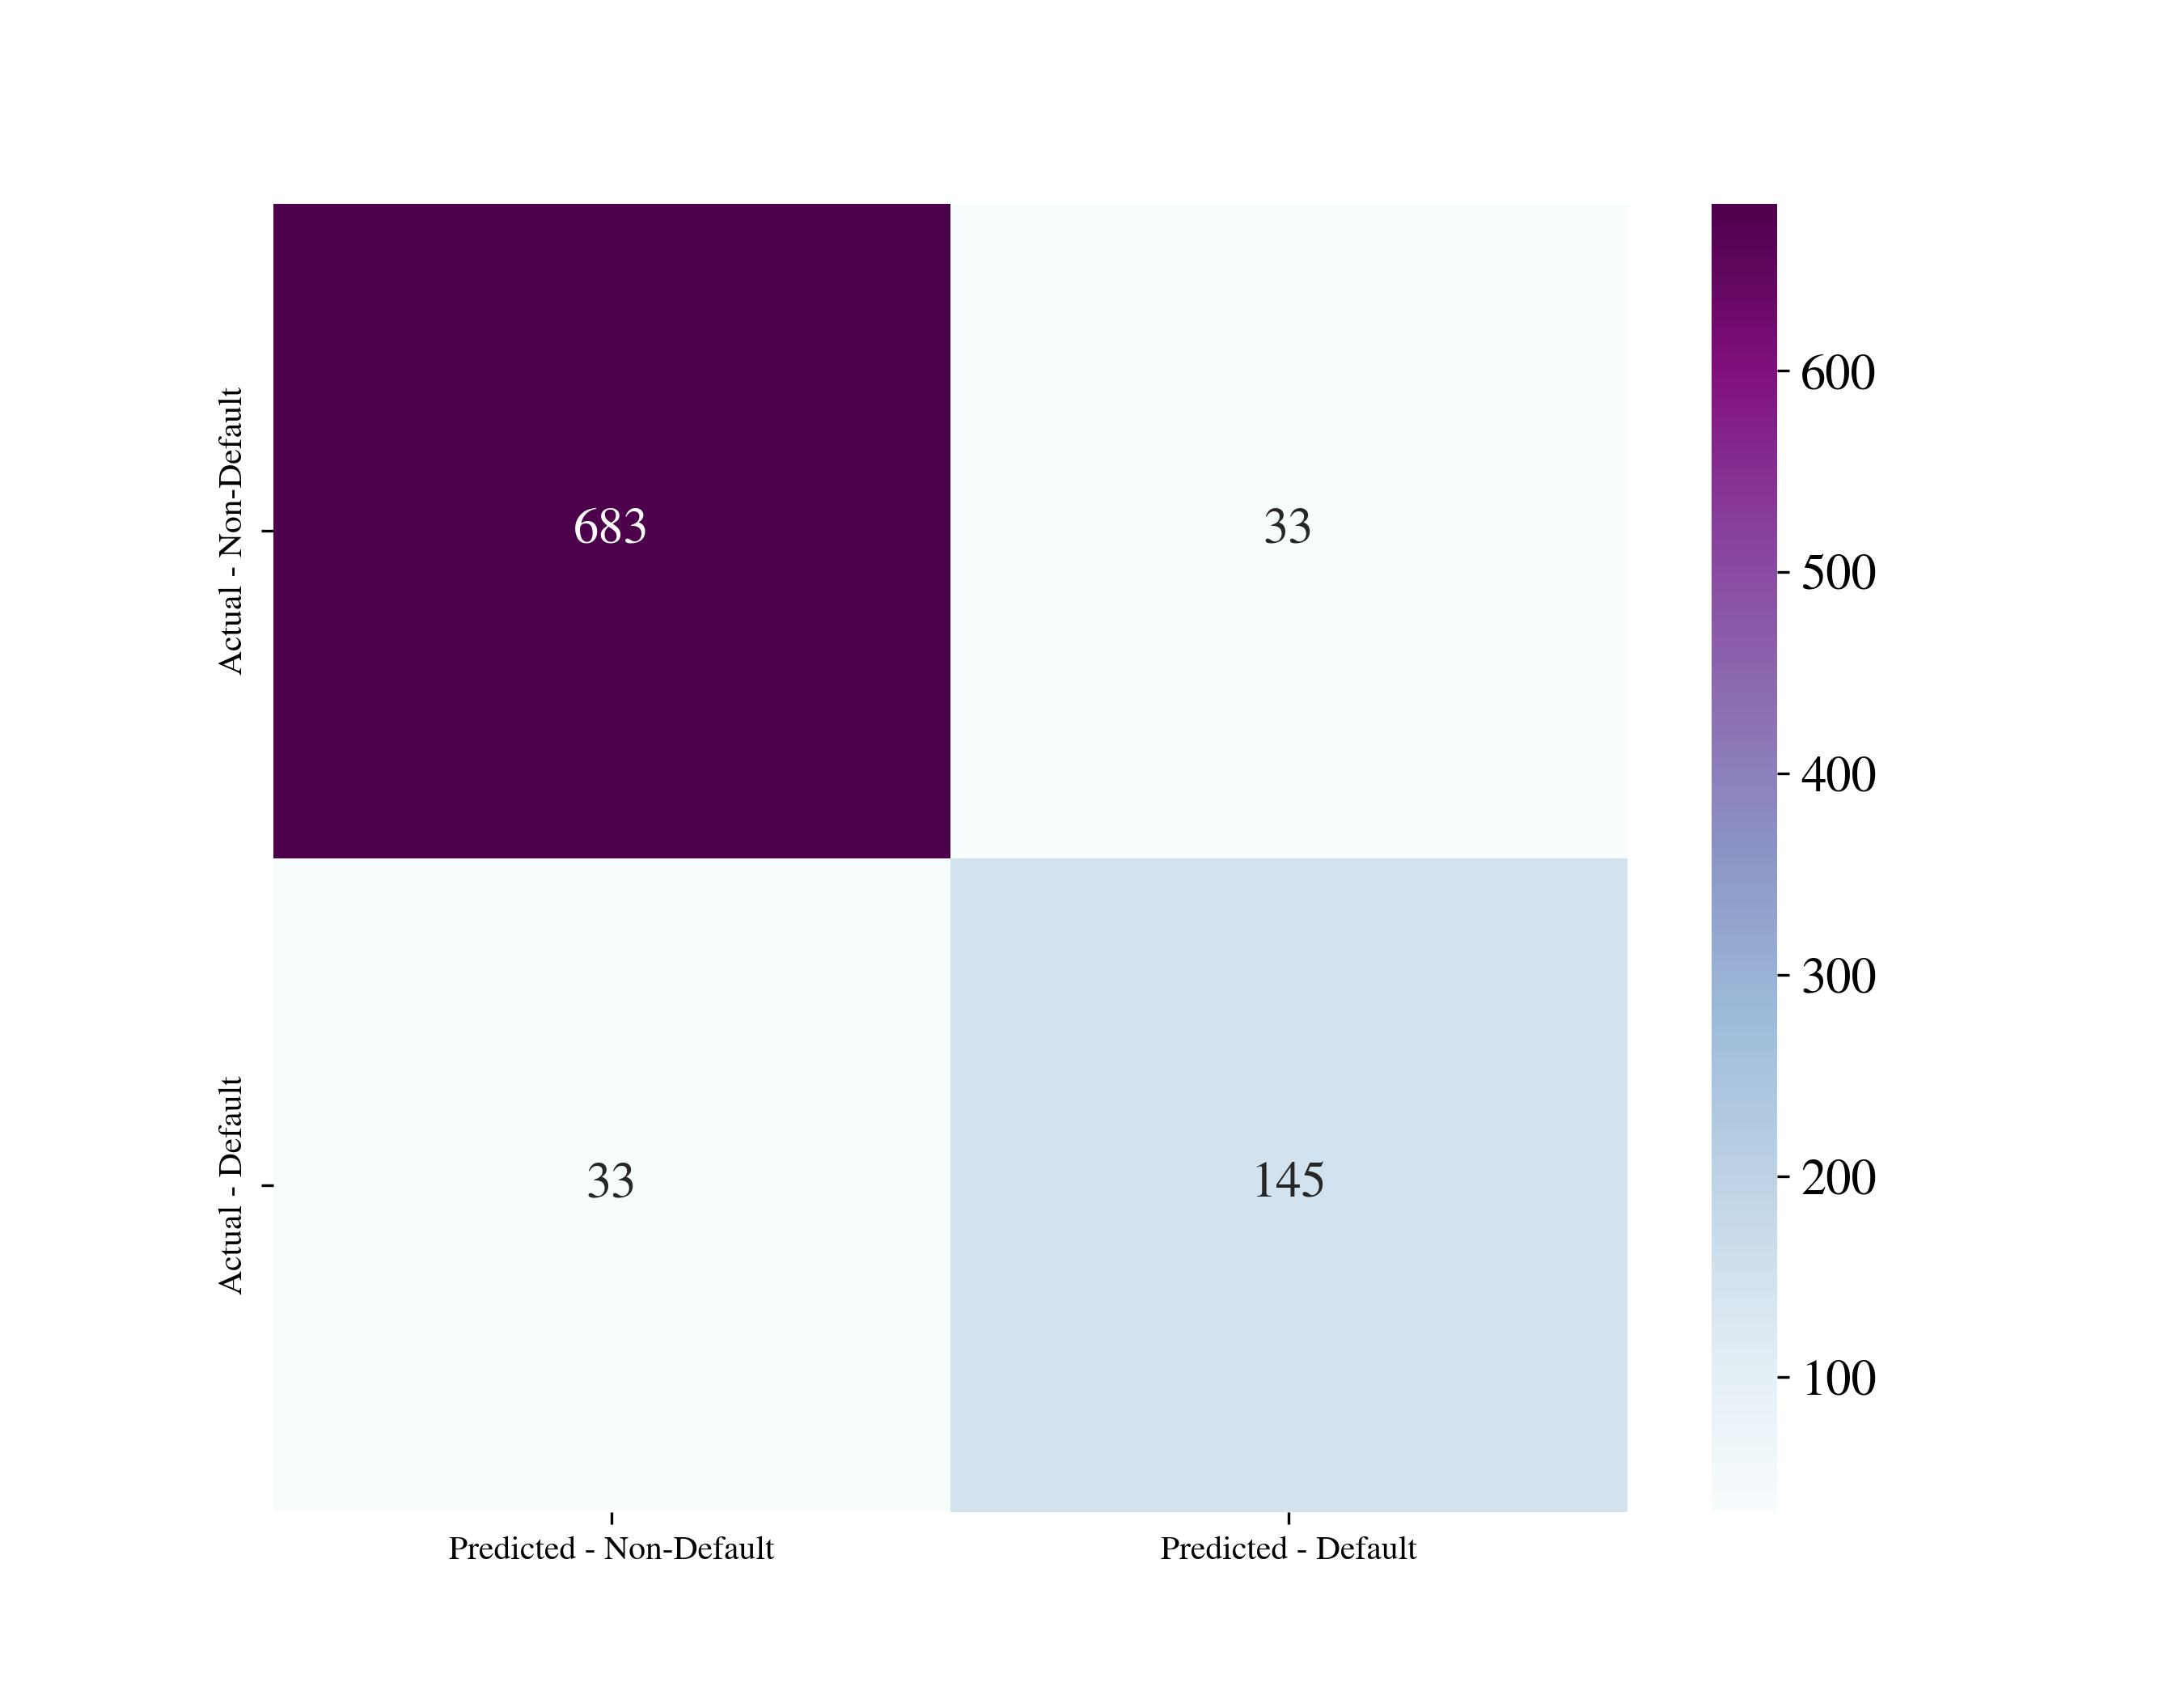
\includegraphics[width=130mm]{Figures/Confusion_Matrix.jpg}
\centering{\begin{source}Author's results in Python\end{source}}\vspace{-1em}
\end{figure}

In order to obtain a better understanding of the model's performance on previously unseen data, we computed several metrics that were used during the model selection process.
These metrics are presented in \autoref{tab:metricseval}. The results indicate that the model performs well on the unseen data, with most of the scores metrics around 80 \% to 90 \%.
Furthermore, the loss metrics are relatively low, indicating that the model can effectively distinguish between defaults and non-defaults.
Overall, these results suggest that the model is performing well and is suitable for predicting defaults.
The results suggest that the model has a good balance between correctly identifying defaults and non-defaults, as well as minimizing false positives and false negatives. This further confirms the model's ability to accurately predict defaults.

\begin{table}[H]
    \small
    \setlength{\tabcolsep}{8pt}
    \renewcommand{\arraystretch}{1.3}
    \centering
        \caption[Metrics Evaluation]{Metrics Evaluation}\label{tab:metricseval}
        \begin{tabular}{@{} r r @{\hspace{1cm}} l @{}}
    \toprule
    \textbf{Metric} & \textbf{Value}\\
    \midrule
    \hline
    F1 & 0.8146 \\ 
    Precision & 0.8146 \\ 
    Recall & 0.8146 \\ 
    Accuracy & 0.9262 \\ 
    AUC & 0.9564 \\ 
    Somers' D & 0.9128 \\ 
    KS & 0.7915 \\ 
    MCC & 0.7685 \\ 
    Brier Score Loss & 0.0594 \\
    Log Loss & 0.2163 \\
    \hline
    \bottomrule
    \end{tabular}
    \vspace{0.35em}

        \centering{\begin{source}Author's results in Python\end{source}}\vspace{-1em}
\end{table}

The following \autoref{tab:recab} shows the impact of recalibration on the model's performance metrics. $M_{NR}$ denotes the final model which was not recalibrated at all (i.e., was trained only on the training set), whereas $M_R$ denotes the recalibrated model (i.e., trained on the joined training and validation set). Respectively, $M_{NR}$ uses its threshold computed bas on the training set (0.4955), and $M_R$ uses its threshold computed on the joined training and validation set(0.45109).
As can be seen, the recalibration indeed has a positive impact on the metrics evaluation as all the metric scores have increased, while the metric loss functions decreased.
We can observe the most significant decrease in the Log Loss function, which decreased by 8.09 \%, while the objective function F1 score has increased by 3.30 \% thanks to to increase in both Precision and Recall.
Therefore, the recalibration process is deemed desired and appropriate in terms of model's performance.

\begin{table}[H]
    \small
    \setlength{\tabcolsep}{8pt}
    \renewcommand{\arraystretch}{1.3}
    \centering
        \caption[Recalibration Impact on Metrics Evaluation]{Recalibration Impact on Metrics Evaluation}\label{tab:recab}
        \begin{tabular}{@{} r r @{\hspace{0.5cm}} r @{\hspace{0.5cm}} r @{}}
            \toprule
            \textbf{Metric} & \textbf{$M_{NR}$} & \textbf{$M_{R}$} & \textbf{Diff.}\\
    \midrule
    \hline
    F1 & 0.7886 & 0.8146 & 3.30 \% \\ 
    Precision & 0.8023 & 0.8146 & 1.53 \% \\ 
    Recall & 0.7753 & 0.8146 & 5.07 \% \\ 
    Accuracy & 0.9172 & 0.9262 & 0.98 \% \\ 
    AUC & 0.9518 & 0.9564  & 0.48 \% \\ 
    Somers' D & 0.9037 & 0.9128 & 1.01 \% \\ 
    KS & 0.7845 & 0.7915 & 0.89 \% \\ 
    MCC & 0.7373 & 0.7685 & 4.23 \% \\ 
    Brier Score Loss & 0.0632 & 0.0594 & -6.11 \% \\
    Log Loss & 0.2353 & 0.2163 & -8.09 \% \\
    \hline
    \bottomrule
    \end{tabular}
    \vspace{0.35em}

        \centering{\begin{source}Author's results in Python\end{source}}\vspace{-1em}
\end{table}

To further evaluate the performance of the (recalibrated) model, we can visualize the ROC curve, as presented in \autoref{fig:roc}. The curve illustrates the trade-off between the true positive rate and the false positive rate at various classification thresholds. An ideal ROC curve should have an area under the curve (AUC) value of 100 \%, indicating a perfect classifier, while a random classifier would have an AUC of 50 \%.

From the curve, we observe that the AUC value of the model is 95.55 \%, indicating a high degree of accuracy in distinguishing between defaults and non-defaults. The curve covers most of the area under the diagonal line, indicating that the model is performing well in differentiating the two classes. Therefore, the results suggest that the model is performing well and is capable of accurately identifying potential defaulters.

\begin{figure}[H]
\centering
\caption{ROC Curve}\vspace{0.5em}
\label{fig:roc}\
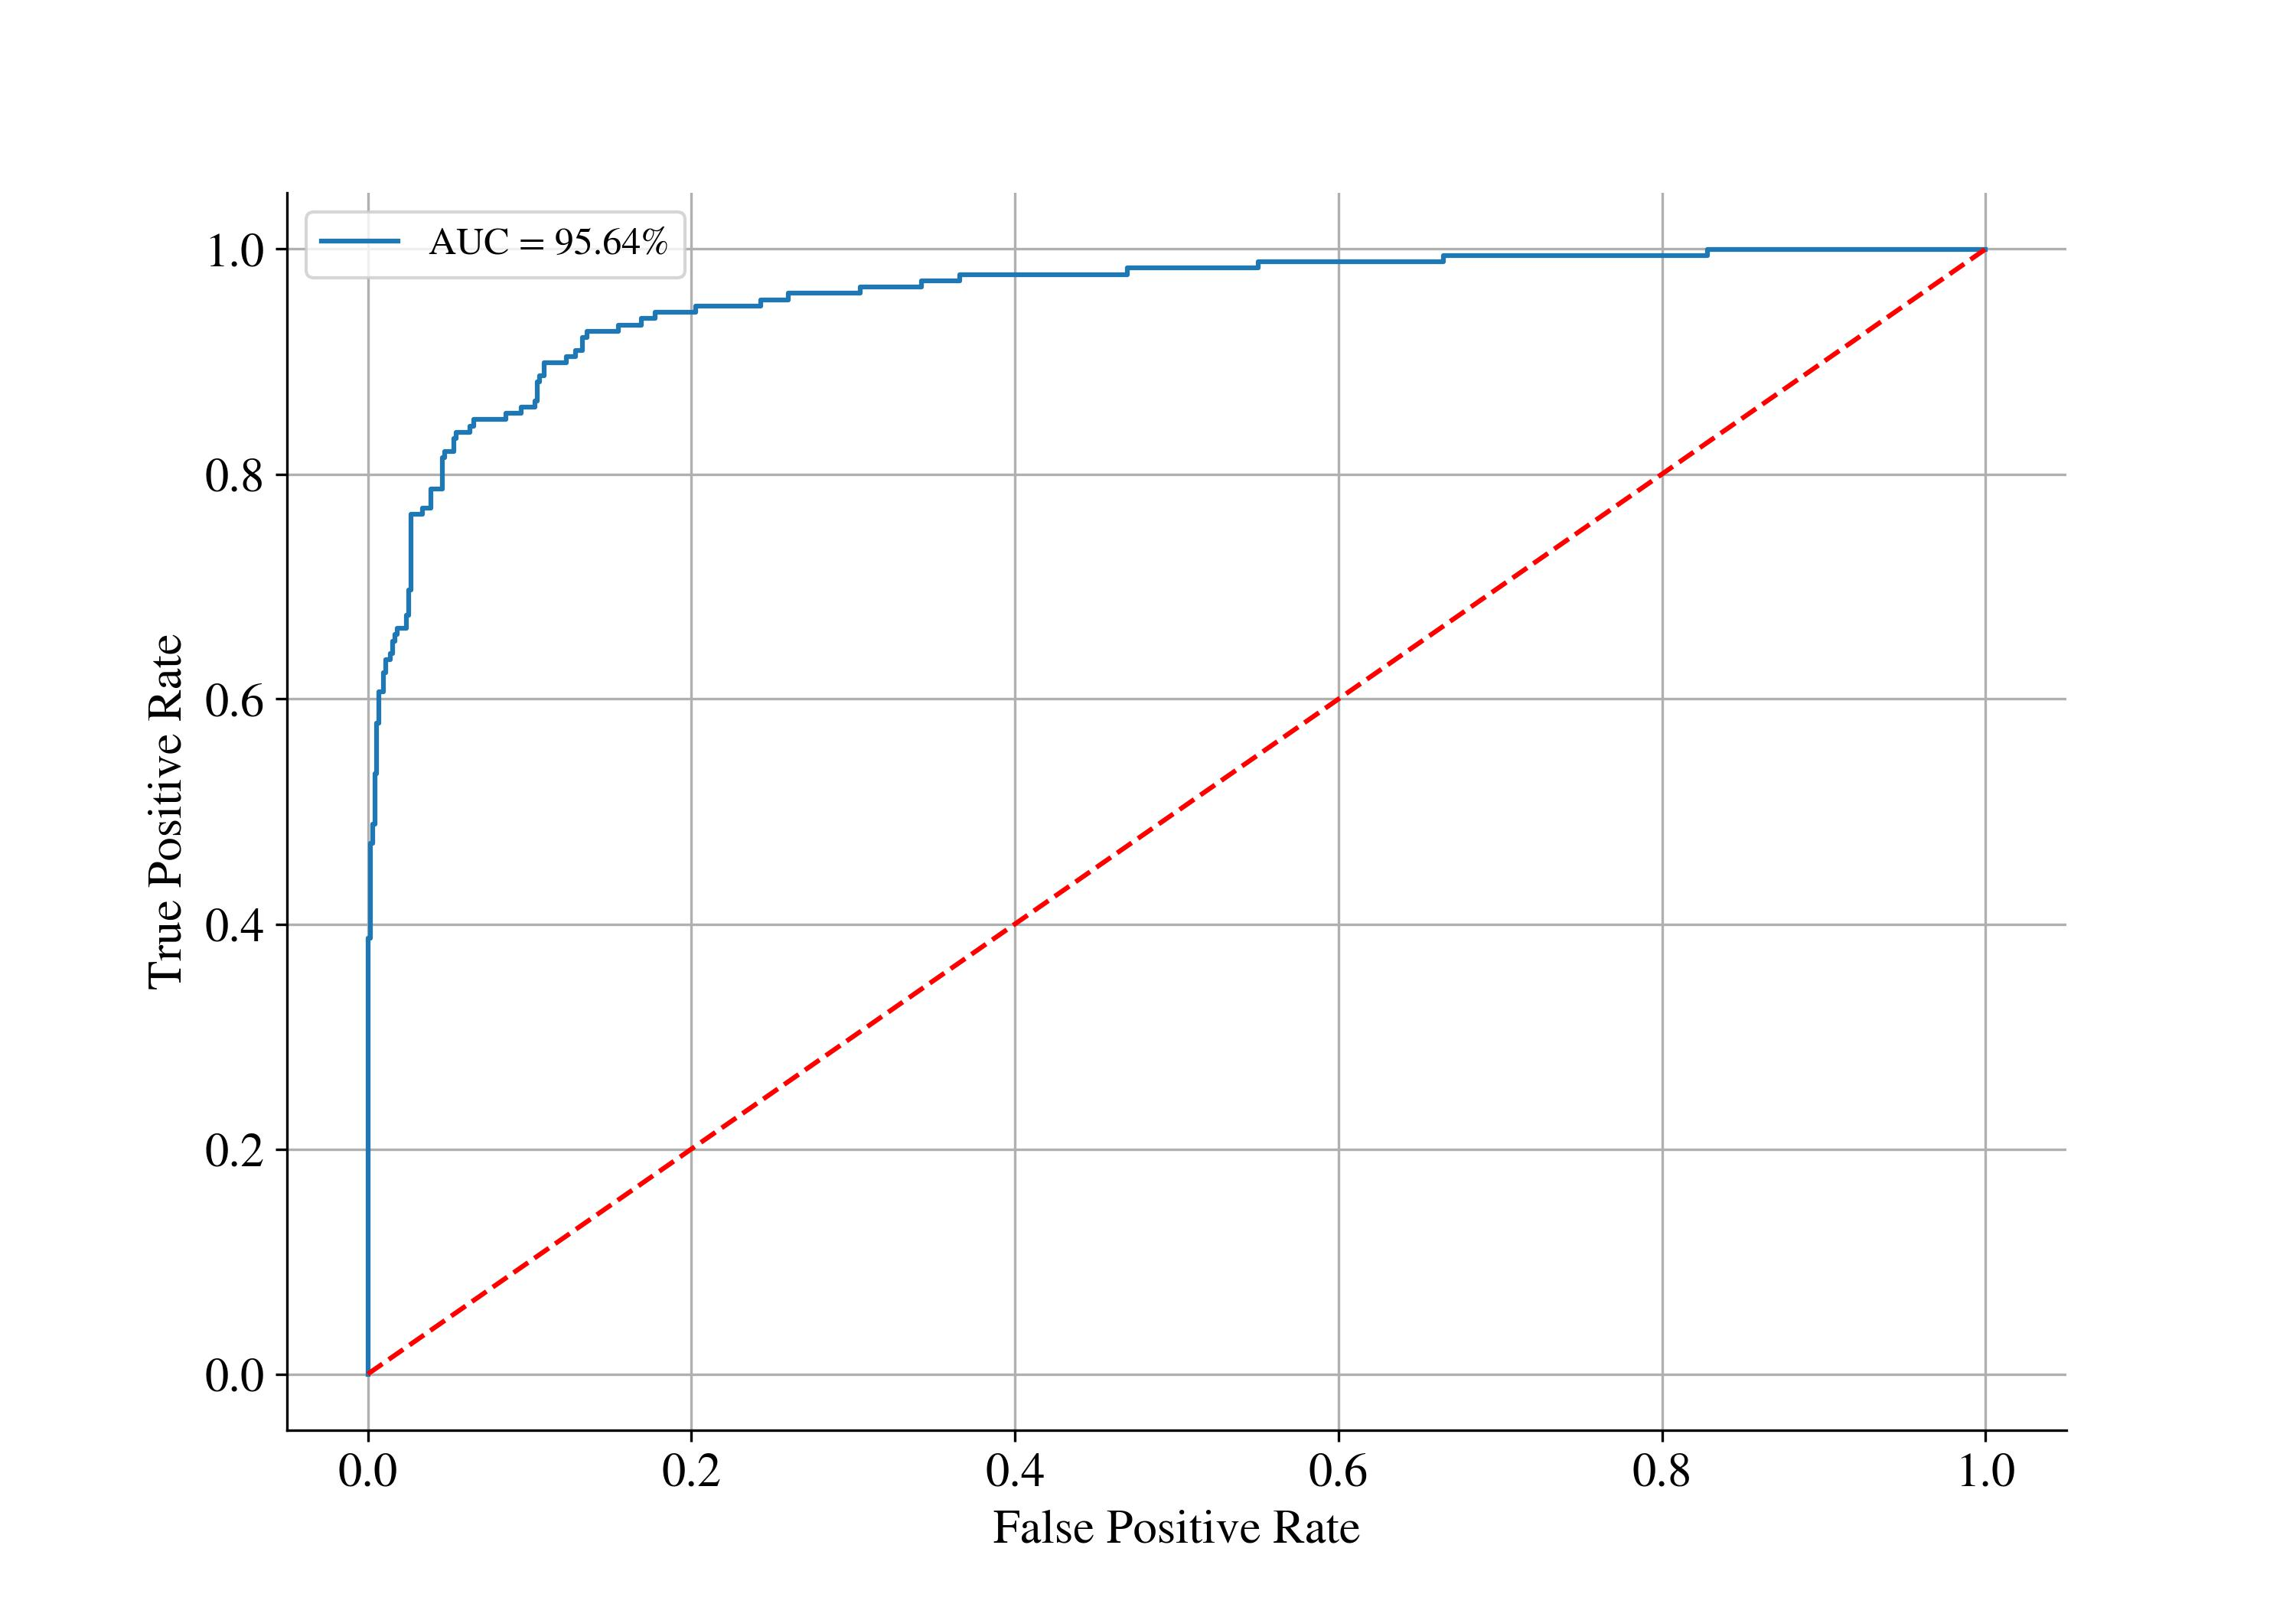
\includegraphics[width=140mm]{Figures/ROC_curve_FINAL.jpg}
\centering{\begin{source}Author's results in Python\end{source}}\vspace{-1em}
\end{figure}

\subsection{Model Explainability}
To gain insights into the impact of the features used in the final model, we can inspect the feature imporances of the final model, which is a part of family of tree ensemble algorithms.
As the names indicates, it is the score value representing the importance of the features, i.e., the higher score, the more important the feature is. Basically, it is the measure of how much a feature contributes to the overall performance of the model.
Overall, the feature importance plot provides valuable insights into the factors that are most important in predicting loan defaults. It can be used to identify which features are contributing the most to the model's accuracy and to guide future feature selection efforts.
According to Bonaccorso \citep{bonaccorso2020mastering}, feature importance is the measure proportional to the impurity reduction that a particular feature allows us to achieve, and is defined as:
\begin{equation}\label{eq}
    \text{FI}\left(\bar{x}^{\left(i\right)}\right) = \frac{1}{N} \displaystyle\sum_{k=1}^{N} \displaystyle\sum_{j=1}^{L} \frac{n(j)}{M} \delta I_{j}^{i}
\end{equation}
where $ \text{FI}\left(\bar{x}^{\left(i\right)}\right)$ referes to the feature importance of the feature $i$, $n(j)$ is the number of samples reaching the node $j$, $\delta I_{j}^{i}$ represents the impurity reduction at node $j$ after the splitting using the feature $j$, $M$ is total number of samples in the data set used to built the model, and $N$ refers to the number of tree estimators used within an ensemble model.

The following \autoref{fig:fi} depicts the feature importances of all the selected features on which the model was trained.
The two most important features used in the final model are \texttt{DEBTINC} and \texttt{DELINQ}, which are crucial delinquency indicators in determining whether a borrower would be able to repay their loan. These two features have a significant impact on the model's ability to accurately predict loan defaults, with high feature importance scores. This is also in line with the findings from the exploratory analysis, WoE distribution or feature selection.
\begin{figure}[H]
\centering
\caption{Feature Importance}\vspace{0.5em}
\label{fig:fi}\
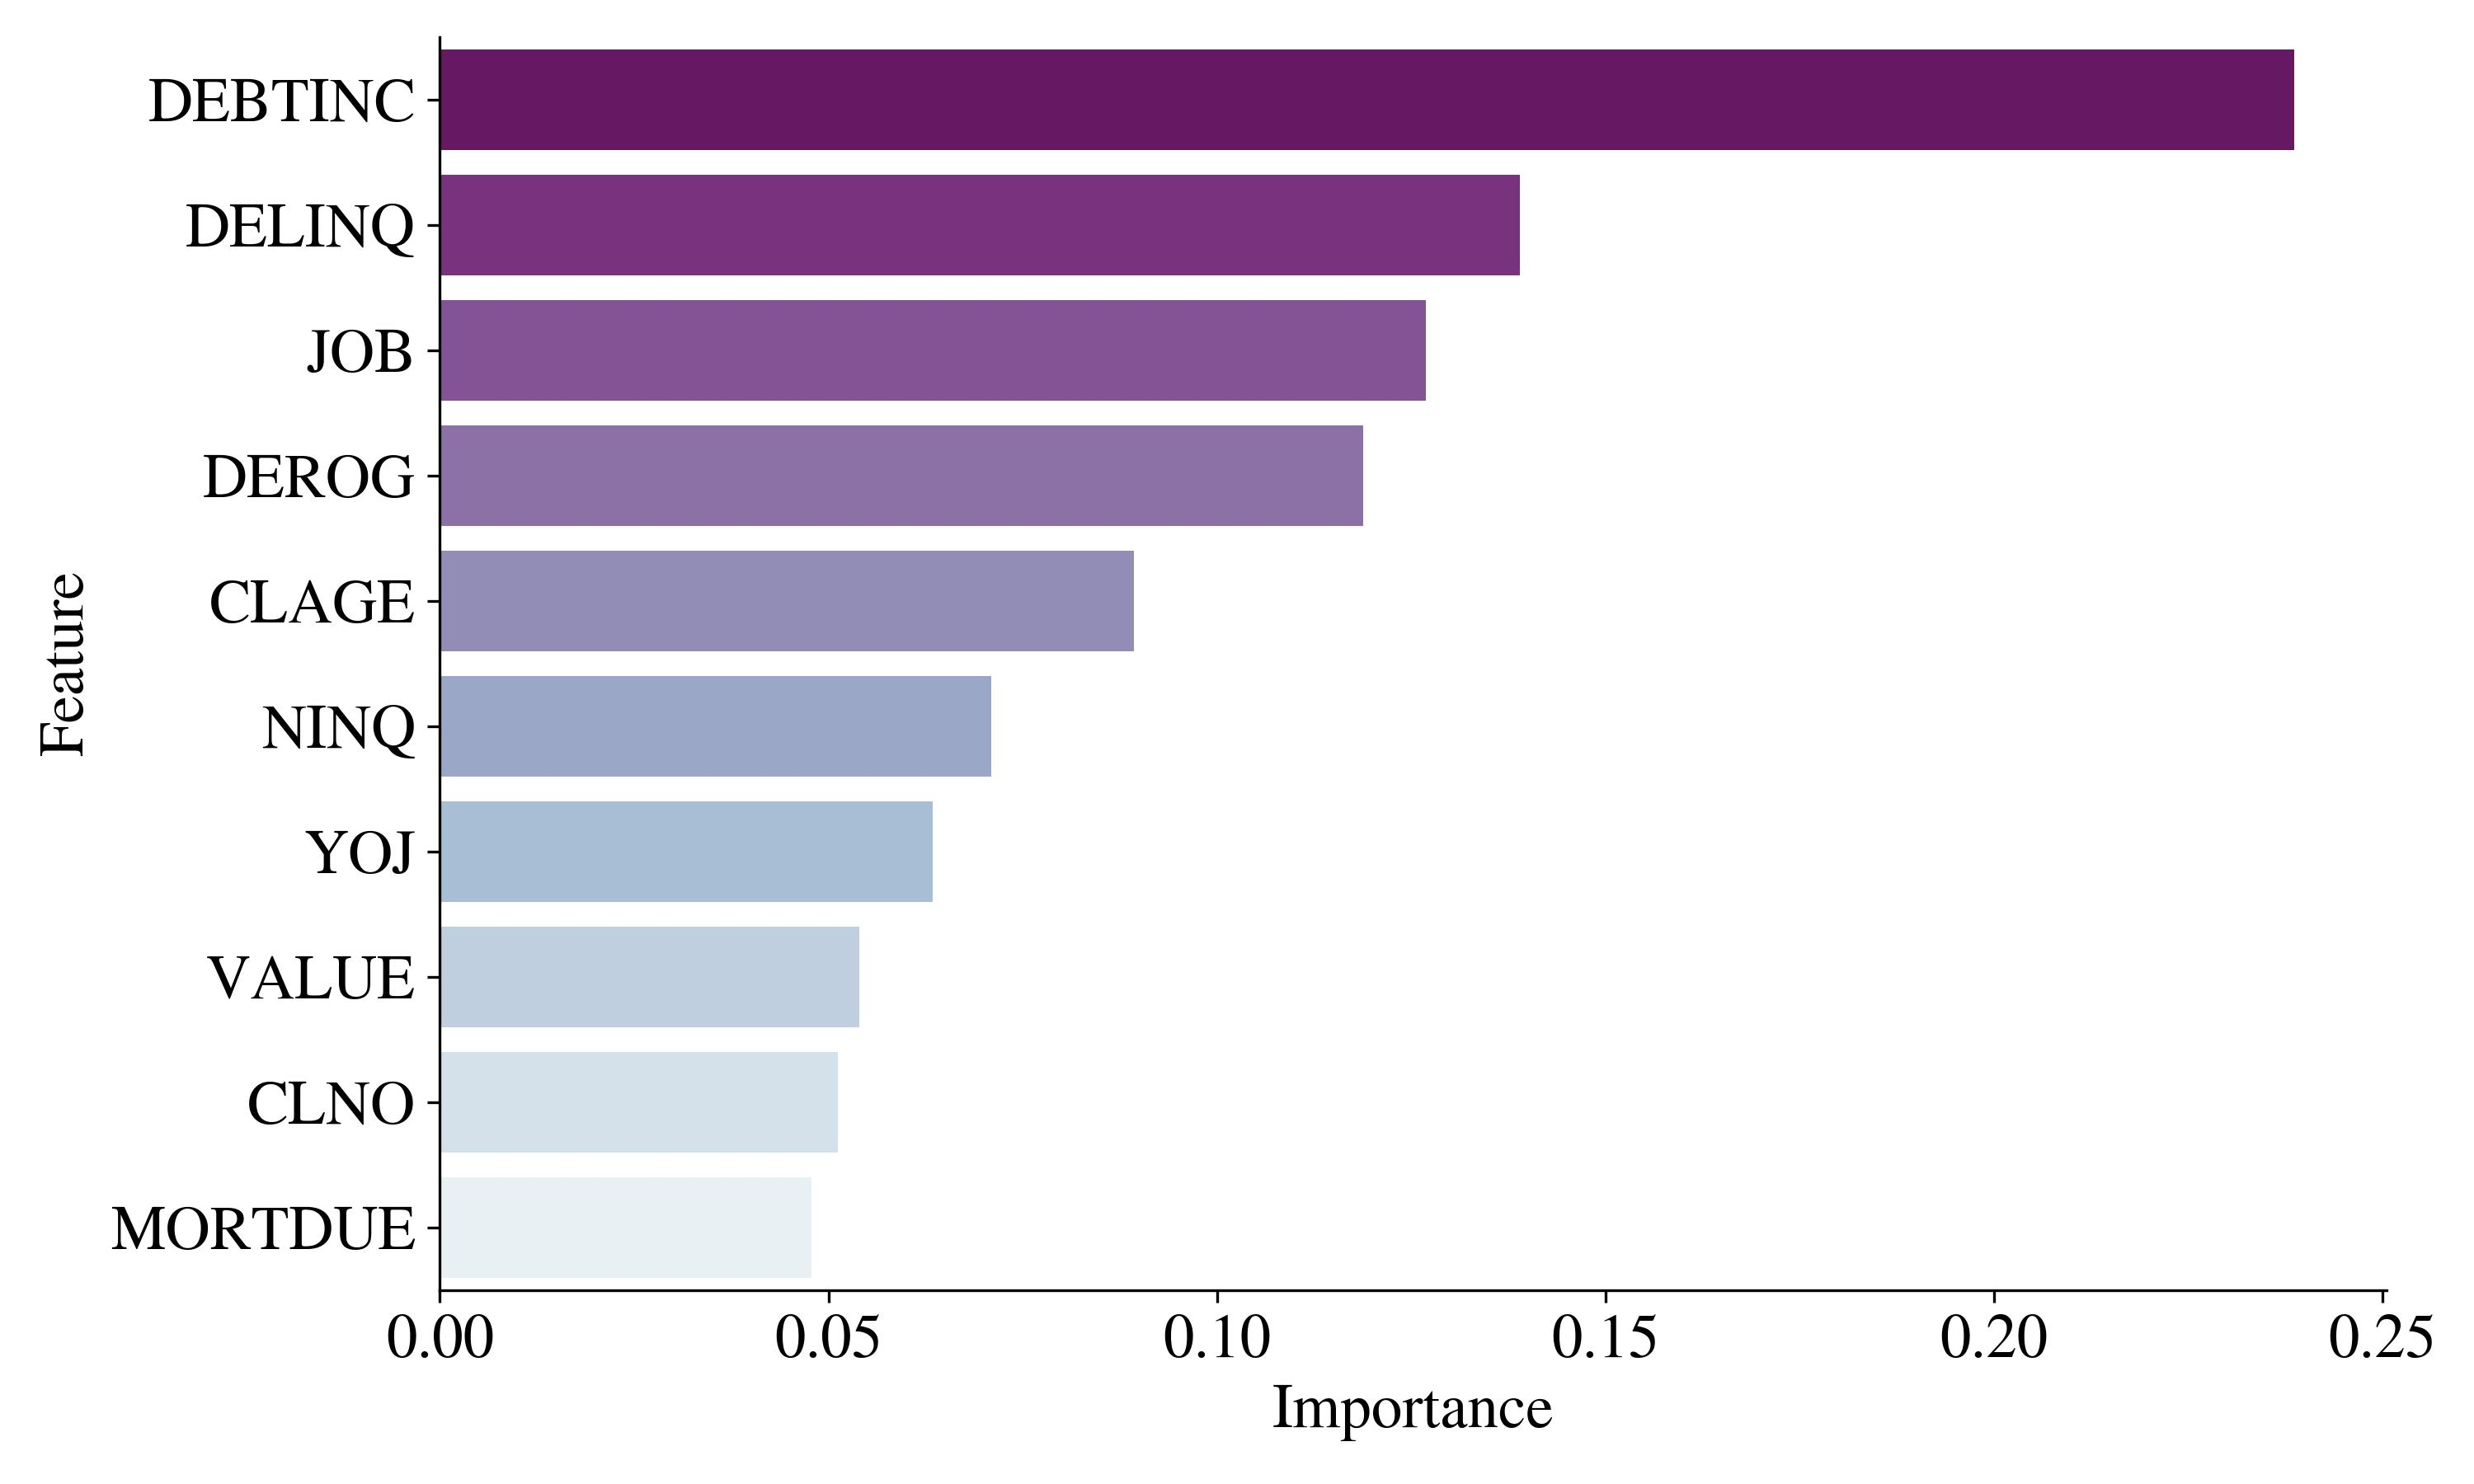
\includegraphics[width=140mm]{Figures/Feature_Importances.jpg}
\centering{\begin{source}Author's results in Python\end{source}}\vspace{-1em}
\end{figure}

Thus, understanding the impact of individual features on model performance can be useful in identifying areas for improvement, as well as in identifying the most significant factors that drive loan defaults.
By focusing on these important features, lenders and policymakers can better understand and address the underlying factors that contribute to default risk, ultimately leading to better lending decisions and improved outcomes for borrowers and lenders alike.

\textbf{ADD BRIEF THEORY ABOUT THE SHAP VALUES}

To gain further insights into the impact of the features on the final model's predictions, the SHapley Additive exPlanations (henceforth SHAP) summary plot is displayed in \autoref{fig:shap}.
The SHAP summary plot provides a clear visualization of the contribution each feature makes to a prediction and is used for a black box model explainability.
Each dot in the plot represents a feature and its corresponding SHAP value.
The color of the dot represents the feature's value, with red indicating high values and blue indicating low values.
The position of the dot on the x-axis represents the impact of the feature on the prediction, with features on the right-hand side contributing more positively to the prediction, and features on the left-hand side contributing more negatively.

Since our data points are encoded in WoE values, the higher (the more positive) value, the larger distribution of non-defaulters compared to defaulters, and vice versa, the lower (the more negative) value, the larger distribution of defaulters compared to non-defaulters.
For the most important features, we can observe that the blue values (negative WoE values) and red values (positive WoE values) are quite separable.
Negative WoE values are positively contributing to the predictions, and the positive WoE values are negatively contributing to the predictions. This means that the more negative the WoE value, the more likely the borrower is to default, and vice versa.

Overall, the SHAP summary plot provides a valuable tool for interpreting and understanding the complex decision-making process of the final model.
The plot enables us to examine the impact of individual features on the model's output and helps us to identify which features are most influential in the model's decision-making process.
By understanding the relative importance of each feature, we can gain deeper insights into the creditworthiness assessment process and make more informed decisions in the lending industry.

\begin{figure}[H]
\centering
\caption{SHAP Summary Plot}\vspace{0.5em}
\label{fig:shap}\
\includegraphics[width=140mm]{Figures/SHAP_summary_plot.jpg}
\centering{\begin{source}Author's results in Python\end{source}}\vspace{-1em}
\end{figure}


\newpage
\section{Machine Learning Deployment}
This section describes the process of taking a trained machine learning model and making it available for use in the real world. It involves taking the model from a development environment and integrating it into a production environment where it can be used to make predictions or decisions based on new data. In this thesis, the machine learning model is deployed as web application using Flask and HTML.
\subsection{Final Model Recalibration}
Before deploying the model in a production setting, a meticulous process is undertaken to ensure optimal performance.
This involves conducting a final recalibration of the model using the entire data set, comprising the training, validation, and test sets.
The purpose of this recalibration is to fine-tune the model parameters, thereby maximizing its ability to generalize and yield accurate predictions.

The test set, which has been employed previously during the model evaluation phase, is incorporated into the recalibration process without any risk of data leakage.
By including the test set, the sample size for training is expanded, thereby increasing the model's capacity to generalize effectively.

Upon completion of the recalibration, the final classification threshold for deployment is determined to be \textbf{0.3358}.
This value is derived from a comprehensive analysis of the training, validation, and test sets, which ensures that the model's generalization capabilities are further enhanced for optimal performance in real-world applications.

\subsection{Flask and HTML Web Application}

In this case, the machine learning model was deployed into a web application using Flask and HTML. The application is temporarily deployed on the Cloud server on the \textbf{PythonAnywhere} platform and is accessible here: \url{http://ml-credit-risk-app-petrngn.pythonanywhere.com/}.
However, the application will be shut down after the thesis defense and will not be available online anymore due to the budget reasons.
Nevertheless, the code for the application is available in the GitHub repository, and the application can be run locally using any Python compiler.

Furthermore, prior to deployment, we need to prepare several Python inputs for the web application, including:
\begin{itemize}\setlength\itemsep{0em}
\item Model - the final model recalibrated on the training, validation and test set.
\item Threshold - the final classification threshold recalibrated on the training, validation and test set.
\item Features - the final features used in the final model.
\item Data Frame - the input tabular object used in the web application to store the loan applicant's inputs.
\item Optimal Binning Transformator - fitted \lstinline{BinningProcess} object for binning and WoE-encoding of the loan applicant's inputs.
\item WoE Bins - a set of bins and WoE values used for mapping the WoE values to missing values.
\end{itemize}

Such inputs required for the machine learning application are exported in the \lstinline{.pkl} format using the \lstinline{pickle} module. This format allows for efficient and easy-to-use serialization and deserialization of the inputs. The pickled file is then loaded directly into the Flask application.

For the back-end of the web application, Flask is used to deploy the machine learning model. The Flask application is coded in the \lstinline{app.py} file, which is stored in the \lstinline{flask_app} repository. The front-end of the web application is coded in HTML, with CSS and JavaScript elements used to enhance the user interface.

The web application first renders an HTML page, as shown in \autoref{fig:flaskform}.
This page contains a loan application form, in which the user or the loan applicant fills in the respective field values that correspond to the features on which the machine learning model was trained.
The form is designed to capture the necessary information required for the model to make a prediction about the loan applicant's application.
Note that not all fields in the loan application form need to be filled out. This is because the missing values in certain features may indicate a higher risk of default. Conversely, one may choose to impose a restriction on the form, requiring all fields to be filled out. However, this could result in a lower number of received applications from delinquent clients, as they may not have all the necessary information to complete the form.
\begin{figure}[H]
\centering
\caption{Flask Web Application Form}\vspace{0.5em}
\label{fig:flaskform}\
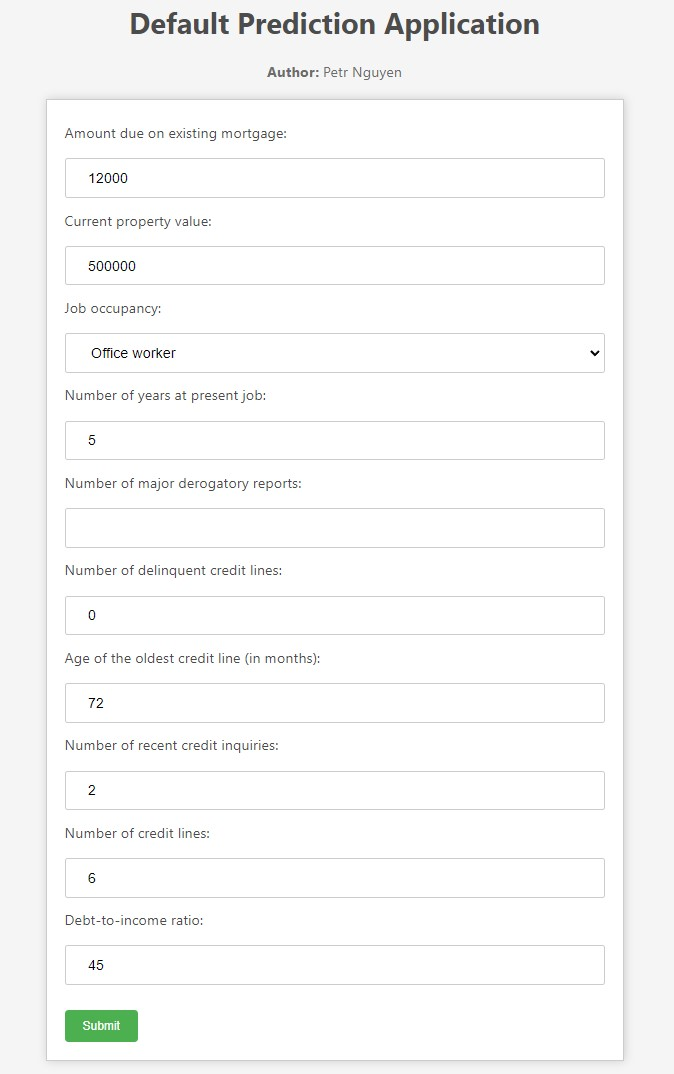
\includegraphics[width=140mm]{Figures/flask_app_form.jpg}

\centering{\begin{source}Author's results in Python\end{source}}\vspace{-1em}
\end{figure}
\clearpage

Once, the loan application form is submitted, the web application uses the pickled input to transform the data from the loan application form and use it in the recalibrated model in order to get the result, whether the given loan applicant would repay his loan based on predetermined threshold. The result is then displayed in the web application, as shown in \autoref{fig:flaskres}.
Particularly, the web application returns whether the loan application would be denied or approved and also the probability score of default.

\begin{figure}[H]
\centering
\caption{Flask Web Application - Prediction Result}\vspace{0.5em}
\label{fig:flaskres}\
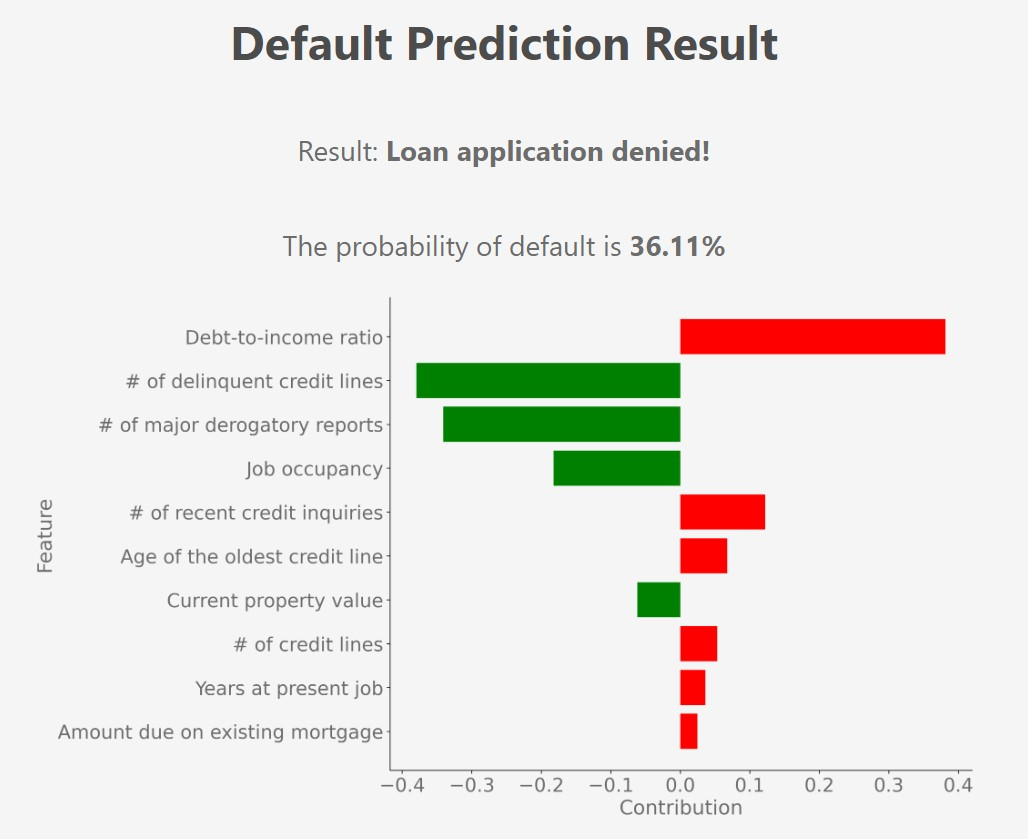
\includegraphics[width=130mm]{Figures/flask_app_result.jpg}

\centering{\begin{source}Author's results in Python\end{source}}\vspace{-1em}
\end{figure}

Besides the prediction results, it also displays the Local Interpretable Model-Agnostic Explanations (henceforth LIME) of the black--box model (Gradient Boosting) with respect to the inputs submitted within the form.
LIME focuses on the local explainability of the black box model around the black--box prediction as it generates a new data set consisting of perturbed samples around the given prediction and then trains a surrogate linear model on the new data set.
Such local interpretable, surrogate model should be a good approximation of the black box model in the vicinity of the given prediction, i.e., the local interpretable model is then used to explain the prediction of the black box model \citep{ribeiro2016should}.

The LIME explanation of input instances $x$ is given as follows:
\begin{equation}\label{eq}
\xi(x) = \arg\min_{g \in G} L(f, g, \pi_x) + \Omega(g)
\end{equation}

where $f$ is the original black--box model, $g$ is the surrogate model, $L$ is the loss functions measuring how far is the explanation $\xi(x)$ far from the prediction produced by black--box model $f$, and $\Omega(g)$ is the complexity of the surrogate model $g$.


The explanation is given in terms of the feature importance, which is represented by the magnitude of the feature's coefficient in the local interpretable model. The higher the magnitude of the coefficient, the more important the feature is in the prediction of the black box model.
Therefore, as it is shown in \autoref{fig:flaskres}, the red bars indicate positive contribution to the probability of default whereas green bars indicate negative contribution to the probability of default. In other words, The features with red bars indicates that the client would not probably repay his loan and vice versa.
The contributions' magnitudes are in line with the findings from feature imporance or SHAP values which is focused on the global explainability of the black--box model (not local explainability), that features such as debt--to--income ratio (\texttt{DEBTINC}) or number of deliquent credit lines (\texttt{DELINQ}) have the largest impact of the probability default.
Particularly, a high value of debt--to--income ratio causes higher probability default, whereas no delinquent credit lines leads to the lower probability default.
